\documentclass[12pt, a4paper,openany]{Thesis} % Paper size, default font size and one-sided paper
%% Change format for two-sided printing
\newcounter{print}
\setcounter{print}{0}    
    % comment out line 2 and give argument 1 for print layout
    % uncomment line 2 and give argument 0 for digital layout
\usepackage{sectsty}
\chapterfont{\centering}
\usepackage{emptypage}
\usepackage{nicefrac}
\usepackage[inkscapeformat=png]{svg}
% \usepackage[none]{hyphenat}
\tolerance=1
\emergencystretch=\maxdimen
\hyphenpenalty=10000
\hbadness=10000


\usepackage[parfill]{parskip}
\setlength{\parindent}{0em}

% \usepackage[resetlabels,labeled]{multibib}

\usepackage[utf8]{inputenc}
\usepackage{wrapfig}
\usepackage{lscape}
\usepackage{rotating}
\usepackage{graphicx, overpic}
\graphicspath{{./Images}} % Specifies the directory where pictures are stored
\usepackage{caption}
\usepackage{amsmath, nccmath}
\usepackage{comment}
% \usepackage{titlefoot}
\usepackage[absolute,overlay]{textpos}
\usepackage{afterpage}
\usepackage{multirow}
\usepackage{multicol}
\usepackage{cleveref}
\usepackage{rotating}
% \usepackage[font=small]{caption}
% \captionsetup{compatibility=false}
\usepackage{subcaption}
\usepackage{float}
\floatstyle{plaintop}
\restylefloat{table}
% \usepackage{subfig}
\usepackage{makecell}
\usepackage{xcolor}
\usepackage{booktabs}
\usepackage{multirow}
\usepackage{lscape}
\usepackage{longtable}
\usepackage{placeins}
\usepackage{adjustbox}
\usepackage{arydshln} % dashed midline
\usepackage{ragged2e}
\usepackage{lipsum}
\usepackage{amsmath, amssymb, amsfonts, amsthm, mathtools, bm}
% \usepackage{mleftright} 
\usepackage{nccmath}
\usepackage{algorithm,algorithmic}
\usepackage{pmat}
\usepackage{mathtools} % To use box inside an aligned environment
\usepackage[shortlabels]{enumitem} % for roman letter lists
% \usepackage{subfig}

\usepackage{tikz}
\usetikzlibrary{shapes,arrows.meta}
\tikzstyle{line} = [draw, -{Latex[length=1mm,width=2mm]}]
\tikzstyle{linedash} = [draw, dash dot]
\newcommand{\customhref}[2][magenta]{\href{#2}{\color{#1}{#2}}}%
% ---------------- chapter headers -------------------- %
\newcommand\myemptypage{
    \newpage
    \null
    \pagestyle{empty}
    % \addtocounter{page}{-1}
    \newpage
    \pagestyle{plain}
    }
\renewcommand{\chaptermark}[1]{\markboth{#1}{}}
\renewcommand{\sectionmark}[1]{\markright{#1}}

% Define a helper command to store the chapter title
\newcommand{\chaptertitle}{}

\renewcommand{\chaptermark}[1]{%
  \markboth{#1}{}%
  \renewcommand{\chaptertitle}{#1}%
}
\newcommand{\sectiontitle}{}

\renewcommand{\sectionmark}[1]{%
  \markboth{#1}{}%
  \renewcommand{\sectiontitle}{#1}%
}
% \makeatletter
% \renewcommand*\l@section{\@dottedtocline{1}{1.5em}{2.3em}}
% \makeatother
%---------------------- Environments ---------------------------%
\makeatletter
\def\th@plain{%
  \thm@notefont{}% same as heading font
  \itshape % body font
}
\def\th@definition{%
  \thm@notefont{\textbf}% same as heading font
  \normalfont % body font
}
\makeatother

\numberwithin{equation}{chapter}
\numberwithin{figure}{chapter}
\numberwithin{table}{chapter}

% \theoremstyle{definition}
% \newtheorem{definition}{Definition}[section]
% \newtheorem{theorem}[definition]{Theorem}
% \newtheorem{lem}[definition]{Lemma}
% \newtheorem{cor}[definition]{Corollary}
% \newtheorem{prop}[definition]{Proposition}
% \newtheorem{exm}[definition]{Example}
% \newtheorem{assumption}[definition]{Assumption}
% \newtheorem{problem}{Problem}
% \newtheorem*{note}{Note}
% \newtheorem*{hint}{Hint}
% \theoremstyle{remark}
% \newtheorem*{sol}{Solution}
% \newtheorem{ax}{Axiom}[section]

% \theoremstyle{remark}
% \newtheorem*{rem}{Remark}
% \newtheorem*{Note}{Note}
% \numberwithin{definition}{chapter}

% ----------------- Custom Commands ------------------- %
\renewcommand{\d}{\, \mathrm{d}}
\newcommand{\I}{\textbf{I}}
\newcommand{\V}{\textbf{V}}
\newcommand{\lex}{\ensuremath>_{\text{lex}}}
\newcommand{\grlex}{\ensuremath>_{\text{grlex}}}
\newcommand{\grevlex}{\ensuremath>_{\text{grevlex}}}
\newcommand{\op}[1]{\operatorname{#1}}
\newcommand{\ditto}[1][.4pt]{\xrfill{#1}~\textquotedbl~\xrfill{#1}}
\newcommand{\suth}{\textsuperscript{th}}
\newcommand{\Grob}{Gr\"{o}bner }
\newcommand{\GrobB}{Gr\"{o}bner Bases}
\newcommand{\GrobBi}{Gr\"{o}bner Basis}
\renewcommand{\algorithmicrequire}{\textbf{Input:}}
\renewcommand{\algorithmicensure}{\textbf{Output:}}

% \renewcommand*{\thefootnote}{\fnsymbol{footnote}}
\addtocontents{toc}{\protect\setcounter{tocdepth}{1}}
\newcommand\at[2]{\left.#1\right|_{#2}}
\renewcommand\qedsymbol{$\blacksquare$}
\newcommand{\tani}{\tan^{-1}}
\newcommand{\sini}{\sin^{-1}}
\newcommand{\cosi}{\cos^{-1}}
\newcommand{\vLine}{\unskip\ \vrule\ }
% \renewcommand{\arraystretch}{1.3}


\newcommand{\XX}[1]{{\bf XX #1 XX}}
\newcommand{\bi}{\begin{itemize}}\newcommand{\ei}{\end{itemize}}
\newcommand{\be}{\begin{equation}}\newcommand{\ee}{\end{equation}}
\newcommand{\bee}{\begin{enumerate}}\newcommand{\eee}{\end{enumerate}}
\newcommand{\bea}{\begin{eqnarray}}\newcommand{\eea}{\end{eqnarray}}
\newcommand{\beas}{\begin{eqnarray*}}\newcommand{\eeas}{\end{eqnarray*}}

%



\newcommand{\bmf}{\mathbf{f}}
\newcommand{\bmu}{\mathbf{u}}
\newcommand{\bmx}{\mathbf{x}}
\newcommand{\bmv}{\mathbf{v}}
\newcommand{\bmw}{\mathbf{w}}
\newcommand{\bmy}{\mathbf{y}}
\newcommand{\bmd}{\mathbf{d}}
\newcommand{\bmr}{\mathbf{r}}
\newcommand{\bmz}{\mathbf{z}}
\newcommand{\bmphi}{\mathbf{\phi}}
\newcommand{\xm}{X_-}
\newcommand{\xp}{X_+}
\newcommand{\um}{U_-}
\newcommand{\ym}{Y_-}
\newcommand{\xmt}{X_-^\top}
\newcommand{\xpt}{X_+^\top}
\newcommand{\umt}{U_-^\top}
\newcommand{\ymt}{Y_-^\top}

%**********************************
\newcommand{\bpi}{\mathbf{\Pi}}
\newcommand{\schur}{\!\mid\!}
\newcommand{\mpi}{\bbm \Pi_{11}&\Pi_{12}\\\Pi_{21}&\Pi_{22}\ebm}
\newcommand{\gi}{^\dagger}
\renewcommand{\S}[1]{\mathbb{S}^{#1}}
\newcommand{\pip}{\Pi_{22}}
\newcommand{\pis}{\Pi\schur\Pi_{22}}
\newcommand{\zs}{\calZ_r(\Pi)}
\DeclareMathOperator{\In}{In}

\definecolor{marine}{rgb}{0.149,0.149,0.804}
\definecolor{fbrick}{rgb}{0.804,0.149,0.149}
\definecolor{apricot}{rgb}{0.98,0.81,0.69}
\definecolor{Blue}{cmyk}{1.,1.,0,0}
\definecolor{amber}{rgb}{1.0, 0.75, 0.0}
\definecolor{applegreen}{rgb}{0.55, 0.71, 0.0}
\definecolor{bananayellow}{rgb}{1.0, 0.88, 0.21}
\definecolor{bittersweet}{rgb}{1.0, 0.44, 0.37}
\definecolor{candyapplered}{rgb}{1.0, 0.03, 0.0}
\definecolor{carminered}{rgb}{1.0, 0.0, 0.22}
\definecolor{carrotorange}{rgb}{0.93, 0.57, 0.13}
\definecolor{goldenyellow}{rgb}{1.0, 0.87, 0.0}
\definecolor{greenpigment}{rgb}{0.0, 0.65, 0.31}
\definecolor{greenhtml}{rgb}{0.0, 0.5, 0.0}


\newcommand{\magenta}[1]{\textcolor{magenta}{#1}}
\newcommand{\fbrick}[1]{\textcolor{fbrick}{#1}}
\newcommand{\marine}[1]{\textcolor{marine}{#1}}
\newcommand{\green}[1]{\textcolor{greenpigment}{#1}}
\newcommand{\gray}[1]{\textcolor{gray}{#1}}

\newcommand{\ciz}{\hspace{5cm}{{\hrule}}\vspace*{4mm}}
\newcommand{\blue}{\textcolor{blue}}
\newcommand{\red}{\textcolor{red}}


\newcommand{\None}{
  \left[\begin{array}{c|c}
    I & \begin{array}{c}
      X_+\\Y_- 
    \end{array}
    \\\hline
    0 & \begin{array}{c}
      -X_-\\-U_- 
    \end{array}
  \end{array}\right]
  \!\!\!
  \bbm
  \Phi_{11} & \Phi_{12}\\
  \Phi_{21} & \Phi_{22}
  \ebm\!\!\!
  \left[\begin{array}{c|c}
    I & \begin{array}{c}
      X_+\\Y_- 
    \end{array}
    \\\hline
    0 & \begin{array}{c}
      -X_-\\-U_- 
    \end{array}
  \end{array}\right]^\top\!\!
}

\newcommand{\systwo}{
  \bbm
  I\\\hline\\[-3mm]
  \begin{matrix}
    A^\top & C^\top\!\\
    B^\top & D^\top\!
  \end{matrix}
  \ebm
}

\newcommand{\sysone}{
  \bbm
  I\\\hline\\[-3mm]
  \begin{matrix}
    A & B\\
    C & D
  \end{matrix}
  \ebm
}




%

%%%%%%%%%%%%%%%%%%%%%%%%%%%%%%%%%%%%%
%%                                 
%%  NEWCOMMANDS                    
%%                                 
%%  version 9  22/01/15           
%%                                 
%%%%%%%%%%%%%%%%%%%%%%%%%%%%%%%%%%%

%%%%%%%%%%%%%%%%%%%%%%%%%%%%%%%%%%%%
%
%
%%%%%%%%%%%%%%%%%%%%%%%%%%%%%%%%%%%



\DeclareMathOperator{\im}{im}
\DeclareMathOperator{\col}{col}
\DeclareMathOperator{\diag}{diag}
\DeclareMathOperator{\bdiag}{blockdiag}
\DeclareMathOperator{\spn}{span}
\DeclareMathOperator{\rank}{rank}
\DeclareMathOperator{\trace}{tr}
\DeclareMathOperator{\card}{card}
\DeclareMathOperator{\dist}{dist}
\DeclareMathOperator{\inte}{int}
\DeclareMathOperator{\clo}{cl}
\DeclareMathOperator{\rint}{rint}
\DeclareMathOperator{\conv}{conv}
\DeclareMathOperator{\cone}{cone}
\DeclareMathOperator{\dom}{dom}
\DeclareMathOperator{\graph}{graph}
\DeclareMathOperator{\dis}{dis}
\DeclareMathOperator{\Real}{Re}
\DeclareMathOperator{\Imag}{Im}




\let\leq\leqslant
\let\geq\geqslant
\let\emptyset\varnothing

%%%%%%%%%%%%%%%%%%%%%%%%%%%%%%%%%%%%%%%%%%%%%%%%
%     \calA
%%%%%%%%%%%%%%%%%%%%%%%%%%%%%%%%%%%%%%%%%%%%%%%%
\newcommand{\calA}{\ensuremath{\mathcal{A}}}
\newcommand{\calB}{\ensuremath{\mathcal{B}}}
\newcommand{\calC}{\ensuremath{\mathcal{C}}}
\newcommand{\calD}{\ensuremath{\mathcal{D}}}
\newcommand{\calE}{\ensuremath{\mathcal{E}}}
\newcommand{\calF}{\ensuremath{\mathcal{F}}}
\newcommand{\calG}{\ensuremath{\mathcal{G}}}
\newcommand{\calH}{\ensuremath{\mathcal{H}}}
\newcommand{\calI}{\ensuremath{\mathcal{I}}}
\newcommand{\calJ}{\ensuremath{\mathcal{J}}}
\newcommand{\calK}{\ensuremath{\mathcal{K}}}
\newcommand{\calL}{\ensuremath{\mathcal{L}}}
\newcommand{\calM}{\ensuremath{\mathcal{M}}}
\newcommand{\calN}{\ensuremath{\mathcal{N}}}
\newcommand{\calO}{\ensuremath{\mathcal{O}}}
\newcommand{\calP}{\ensuremath{\mathcal{P}}}
\newcommand{\calQ}{\ensuremath{\mathcal{Q}}}
\newcommand{\calR}{\ensuremath{\mathcal{R}}}
\newcommand{\calS}{\ensuremath{\mathcal{S}}}
\newcommand{\calT}{\ensuremath{\mathcal{T}}}
\newcommand{\calU}{\ensuremath{\mathcal{U}}}
\newcommand{\calV}{\ensuremath{\mathcal{V}}}
\newcommand{\calW}{\ensuremath{\mathcal{W}}}
\newcommand{\calX}{\ensuremath{\mathcal{X}}}
\newcommand{\calY}{\ensuremath{\mathcal{Y}}}
\newcommand{\calZ}{\ensuremath{\mathcal{Z}}}
%%%%%%%%%%%%%%%%%%%%%%%%%%%%%%%%%%%%%%%%%%%%%%%%
%     \sfA
%%%%%%%%%%%%%%%%%%%%%%%%%%%%%%%%%%%%%%%%%%%%%%%%
\newcommand{\sfA}{\ensuremath{\mathsf{A}}}
\newcommand{\sfB}{\ensuremath{\mathsf{B}}}
\newcommand{\sfC}{\ensuremath{\mathsf{C}}}
\newcommand{\sfD}{\ensuremath{\mathsf{D}}}
\newcommand{\sfE}{\ensuremath{\mathsf{E}}}
\newcommand{\sfF}{\ensuremath{\mathsf{F}}}
\newcommand{\sfG}{\ensuremath{\mathsf{G}}}
\newcommand{\sfH}{\ensuremath{\mathsf{H}}}
\newcommand{\sfI}{\ensuremath{\mathsf{I}}}
\newcommand{\sfJ}{\ensuremath{\mathsf{J}}}
\newcommand{\sfK}{\ensuremath{\mathsf{K}}}
\newcommand{\sfL}{\ensuremath{\mathsf{L}}}
\newcommand{\sfM}{\ensuremath{\mathsf{M}}}
\newcommand{\sfN}{\ensuremath{\mathsf{N}}}
\newcommand{\sfO}{\ensuremath{\mathsf{O}}}
\newcommand{\sfP}{\ensuremath{\mathsf{P}}}
\newcommand{\sfQ}{\ensuremath{\mathsf{Q}}}
\newcommand{\sfR}{\ensuremath{\mathsf{R}}}
\newcommand{\sfS}{\ensuremath{\mathsf{S}}}
\newcommand{\sfT}{\ensuremath{\mathsf{T}}}
\newcommand{\sfU}{\ensuremath{\mathsf{U}}}
\newcommand{\sfV}{\ensuremath{\mathsf{V}}}
\newcommand{\sfW}{\ensuremath{\mathsf{W}}}
\newcommand{\sfX}{\ensuremath{\mathsf{X}}}
\newcommand{\sfY}{\ensuremath{\mathsf{Y}}}
\newcommand{\sfZ}{\ensuremath{\mathsf{Z}}}
%%%%%%%%%%%%%%%%%%%%%%%%%%%%%%%%%%%%%%%%%%%%%%%%
%     \hata
%%%%%%%%%%%%%%%%%%%%%%%%%%%%%%%%%%%%%%%%%%%%%%%%
\newcommand{\hata}{\ensuremath{\hat{a}}}
\newcommand{\hatb}{\ensuremath{\hat{b}}}
\newcommand{\hatc}{\ensuremath{\hat{c}}}
\newcommand{\hatd}{\ensuremath{\hat{d}}}
\newcommand{\hate}{\ensuremath{\hat{e}}}
\newcommand{\hatf}{\ensuremath{\hat{f}}}
\newcommand{\hatg}{\ensuremath{\hat{g}}}
\newcommand{\hath}{\ensuremath{\hat{h}}}
\newcommand{\hati}{\ensuremath{\hat{i}}}
\newcommand{\hatj}{\ensuremath{\hat{j}}}
\newcommand{\hatk}{\ensuremath{\hat{k}}}
\newcommand{\hatl}{\ensuremath{\hat{l}}}
\newcommand{\hatm}{\ensuremath{\hat{m}}}
\newcommand{\hatn}{\ensuremath{\hat{n}}}
\newcommand{\hato}{\ensuremath{\hat{o}}}
\newcommand{\hatp}{\ensuremath{\hat{p}}}
\newcommand{\hatq}{\ensuremath{\hat{q}}}
\newcommand{\hatr}{\ensuremath{\hat{r}}}
\newcommand{\hats}{\ensuremath{\hat{s}}}
\newcommand{\hatt}{\ensuremath{\hat{t}}}
\newcommand{\hatu}{\ensuremath{\hat{u}}}
\newcommand{\hatv}{\ensuremath{\hat{v}}}
\newcommand{\hatw}{\ensuremath{\hat{w}}}
\newcommand{\hatx}{\ensuremath{\hat{x}}}
\newcommand{\haty}{\ensuremath{\hat{y}}}
\newcommand{\hatz}{\ensuremath{\hat{z}}}
%%%%%%%%%%%%%%%%%%%%%%%%%%%%%%%%%%%%%%%%%%%%%%%%
%     \hatA
%%%%%%%%%%%%%%%%%%%%%%%%%%%%%%%%%%%%%%%%%%%%%%%%
\newcommand{\hatA}{\ensuremath{\hat{A}}}
\newcommand{\hatB}{\ensuremath{\hat{B}}}
\newcommand{\hatC}{\ensuremath{\hat{C}}}
\newcommand{\hatD}{\ensuremath{\hat{D}}}
\newcommand{\hatE}{\ensuremath{\hat{E}}}
\newcommand{\hatF}{\ensuremath{\hat{F}}}
\newcommand{\hatG}{\ensuremath{\hat{G}}}
\newcommand{\hatH}{\ensuremath{\hat{H}}}
\newcommand{\hatI}{\ensuremath{\hat{I}}}
\newcommand{\hatJ}{\ensuremath{\hat{J}}}
\newcommand{\hatK}{\ensuremath{\hat{K}}}
\newcommand{\hatL}{\ensuremath{\hat{L}}}
\newcommand{\hatM}{\ensuremath{\hat{M}}}
\newcommand{\hatN}{\ensuremath{\hat{N}}}
\newcommand{\hatO}{\ensuremath{\hat{O}}}
\newcommand{\hatP}{\ensuremath{\hat{P}}}
\newcommand{\hatQ}{\ensuremath{\hat{Q}}}
\newcommand{\hatR}{\ensuremath{\hat{R}}}
\newcommand{\hatS}{\ensuremath{\hat{S}}}
\newcommand{\hatT}{\ensuremath{\hat{T}}}
\newcommand{\hatU}{\ensuremath{\hat{U}}}
\newcommand{\hatV}{\ensuremath{\hat{V}}}
\newcommand{\hatW}{\ensuremath{\hat{W}}}
\newcommand{\hatX}{\ensuremath{\hat{X}}}
\newcommand{\hatY}{\ensuremath{\hat{Y}}}
\newcommand{\hatZ}{\ensuremath{\hat{Z}}}
%%%%%%%%%%%%%%%%%%%%%%%%%%%%%%%%%%%%%%%%%%%%%%%%
%     \bara
%%%%%%%%%%%%%%%%%%%%%%%%%%%%%%%%%%%%%%%%%%%%%%%%
\newcommand{\bara}{\ensuremath{\bar{a}}}
\newcommand{\barb}{\ensuremath{\bar{b}}}
\newcommand{\barc}{\ensuremath{\bar{c}}}
\newcommand{\bard}{\ensuremath{\bar{d}}}
\newcommand{\bare}{\ensuremath{\bar{e}}}
\newcommand{\barf}{\ensuremath{\bar{f}}}
\newcommand{\barg}{\ensuremath{\bar{g}}}
\newcommand{\barh}{\ensuremath{\bar{h}}}
\newcommand{\bari}{\ensuremath{\bar{i}}}
\newcommand{\barj}{\ensuremath{\bar{j}}}
\newcommand{\bark}{\ensuremath{\bar{k}}}
\newcommand{\barl}{\ensuremath{\bar{l}}}
\newcommand{\barm}{\ensuremath{\bar{m}}}
\newcommand{\barn}{\ensuremath{\bar{n}}}
\newcommand{\baro}{\ensuremath{\bar{o}}}
\newcommand{\barp}{\ensuremath{\bar{p}}}
\newcommand{\barq}{\ensuremath{\bar{q}}}
\newcommand{\barr}{\ensuremath{\bar{r}}}
\newcommand{\bars}{\ensuremath{\bar{s}}}
\newcommand{\bart}{\ensuremath{\bar{t}}}
\newcommand{\baru}{\ensuremath{\bar{u}}}
\newcommand{\barv}{\ensuremath{\bar{v}}}
\newcommand{\barw}{\ensuremath{\bar{w}}}
\newcommand{\barx}{\ensuremath{\bar{x}}}
\newcommand{\bary}{\ensuremath{\bar{y}}}
\newcommand{\barz}{\ensuremath{\bar{z}}}
%%%%%%%%%%%%%%%%%%%%%%%%%%%%%%%%%%%%%%%%%%%%%%%%
%     \barA
%%%%%%%%%%%%%%%%%%%%%%%%%%%%%%%%%%%%%%%%%%%%%%%%
\newcommand{\barA}{\ensuremath{\bar{A}}}
\newcommand{\barB}{\ensuremath{\bar{B}}}
\newcommand{\barC}{\ensuremath{\bar{C}}}
\newcommand{\barD}{\ensuremath{\bar{D}}}
\newcommand{\barE}{\ensuremath{\bar{E}}}
\newcommand{\barF}{\ensuremath{\bar{F}}}
\newcommand{\barG}{\ensuremath{\bar{G}}}
\newcommand{\barH}{\ensuremath{\bar{H}}}
\newcommand{\barI}{\ensuremath{\bar{I}}}
\newcommand{\barJ}{\ensuremath{\bar{J}}}
\newcommand{\barK}{\ensuremath{\bar{K}}}
\newcommand{\barL}{\ensuremath{\bar{L}}}
\newcommand{\barM}{\ensuremath{\bar{M}}}
\newcommand{\barN}{\ensuremath{\bar{N}}}
\newcommand{\barO}{\ensuremath{\bar{O}}}
\newcommand{\barP}{\ensuremath{\bar{P}}}
\newcommand{\barQ}{\ensuremath{\bar{Q}}}
\newcommand{\barR}{\ensuremath{\bar{R}}}
\newcommand{\barS}{\ensuremath{\bar{S}}}
\newcommand{\barT}{\ensuremath{\bar{T}}}
\newcommand{\barU}{\ensuremath{\bar{U}}}
\newcommand{\barV}{\ensuremath{\bar{V}}}
\newcommand{\barW}{\ensuremath{\bar{W}}}
\newcommand{\barX}{\ensuremath{\bar{X}}}
\newcommand{\barY}{\ensuremath{\bar{Y}}}
\newcommand{\barZ}{\ensuremath{\bar{Z}}}
%%%%%%%%%%%%%%%%%%%%%%%%%%%%%%%%%%%%%%%%%%%%%%%%
%     \bbA
%%%%%%%%%%%%%%%%%%%%%%%%%%%%%%%%%%%%%%%%%%%%%%%%
\newcommand{\bbA}{\ensuremath{\mathbb{A}}}
\newcommand{\bbB}{\ensuremath{\mathbb{B}}}
\newcommand{\bbC}{\ensuremath{\mathbb{C}}}
\newcommand{\bbD}{\ensuremath{\mathbb{D}}}
\newcommand{\bbE}{\ensuremath{\mathbb{E}}}
\newcommand{\bbF}{\ensuremath{\mathbb{F}}}
\newcommand{\bbG}{\ensuremath{\mathbb{G}}}
\newcommand{\bbH}{\ensuremath{\mathbb{H}}}
\newcommand{\bbI}{\ensuremath{\mathbb{I}}}
\newcommand{\bbJ}{\ensuremath{\mathbb{J}}}
\newcommand{\bbK}{\ensuremath{\mathbb{K}}}
\newcommand{\bbL}{\ensuremath{\mathbb{L}}}
\newcommand{\bbM}{\ensuremath{\mathbb{M}}}
\newcommand{\bbN}{\ensuremath{\mathbb{N}}}
\newcommand{\bbO}{\ensuremath{\mathbb{O}}}
\newcommand{\bbP}{\ensuremath{\mathbb{P}}}
\newcommand{\bbQ}{\ensuremath{\mathbb{Q}}}
\newcommand{\bbR}{\ensuremath{\mathbb{R}}}
\newcommand{\bbS}{\ensuremath{\mathbb{S}}}
\newcommand{\bbT}{\ensuremath{\mathbb{T}}}
\newcommand{\bbU}{\ensuremath{\mathbb{U}}}
\newcommand{\bbV}{\ensuremath{\mathbb{V}}}
\newcommand{\bbW}{\ensuremath{\mathbb{W}}}
\newcommand{\bbX}{\ensuremath{\mathbb{X}}}
\newcommand{\bbY}{\ensuremath{\mathbb{Y}}}
\newcommand{\bbZ}{\ensuremath{\mathbb{Z}}}

%%%%%%%%%%%%%%%%%%%%%%%%%%%%%%%%%%%%%%%%%%%%%%%%
%     \tta
%%%%%%%%%%%%%%%%%%%%%%%%%%%%%%%%%%%%%%%%%%%%%%%%
\newcommand{\tta}{{\tt a}}
\newcommand{\ttb}{{\tt b}}
\newcommand{\ttc}{{\tt c}}
\newcommand{\ttd}{{\tt d}}
\newcommand{\tte}{{\tt e}}
\newcommand{\ttf}{{\tt f}}
\newcommand{\ttg}{{\tt g}}
\newcommand{\tth}{{\tt h}}
\newcommand{\tti}{{\tt i}}
\newcommand{\ttj}{{\tt j}}
\newcommand{\ttk}{{\tt k}}
\newcommand{\ttl}{{\tt l}}
\newcommand{\ttm}{{\tt m}}
\newcommand{\ttn}{{\tt n}}
\newcommand{\tto}{{\tt o}}
\newcommand{\ttp}{{\tt p}}
\newcommand{\ttq}{{\tt q}}
\newcommand{\ttr}{{\tt r}}
\newcommand{\tts}{{\tt s}}
\newcommand{\ttt}{{\tt t}}
\newcommand{\ttu}{{\tt u}}
\newcommand{\ttv}{{\tt v}}
\newcommand{\ttw}{{\tt w}}
\newcommand{\ttx}{{\tt x}}
\newcommand{\tty}{{\tt y}}
\newcommand{\ttz}{{\tt z}}


%%%%%%%%%%%%%%%%%%%%%%%%%%%%%%%%%%%%%%%%%%%%%
% ENVIRONMENTS
%%%%%%%%%%%%%%%%%%%%%%%%%%%%%%%%%%%%%%%%%%%%%
\newcommand{\bmat}{\begin{matrix}}
\newcommand{\emat}{\end{matrix}}
\newcommand{\bbm}{\begin{bmatrix}}
\newcommand{\ebm}{\end{bmatrix}}
\newcommand{\bbma}{\begin{bmatrix*}[r]}
\newcommand{\ebma}{\end{bmatrix*}}
\newcommand{\bpm}{\begin{pmatrix}}
\newcommand{\epm}{\end{pmatrix}}
\newcommand{\bvm}{\begin{vmatrix}}
\newcommand{\evm}{\end{vmatrix}}
\newcommand{\bse}{\begin{subequations}}
\newcommand{\ese}{\end{subequations}}
\newcommand{\beq}{\begin{equation}}
\newcommand{\eeq}{\end{equation}}
\newcommand{\ben}{\renewcommand{\labelenumi}{\arabic{enumi}.}
\renewcommand{\theenumi}{\arabic{enumi}}\begin{enumerate}}

\newcommand{\een}{\end{enumerate}}

\newcommand{\beni}{\renewcommand{\labelenumi}{\roman{enumi}.}
\renewcommand{\theenumi}{\roman{enumi}}\begin{enumerate}}

\newcommand{\eeni}{\end{enumerate}}

\newcommand{\bena}{\renewcommand{\labelenumi}{\alph{enumi}.}
\renewcommand{\theenumi}{\alph{enumi}}\begin{enumerate}}

\newcommand{\eena}{\end{enumerate}}

\newcommand{\bit}{\begin{itemize}}
\newcommand{\eit}{\end{itemize}}
\newcommand{\bthe}{\begin{theorem}}
\newcommand{\ethe}{\end{theorem}}
\newcommand{\blem}{\begin{lemma}}
\newcommand{\elem}{\end{lemma}}
\newcommand{\bprop}{\begin{proposition}}
\newcommand{\eprop}{\end{proposition}}
\newcommand{\bex}{\begin{example}}
\newcommand{\eex}{\end{example}}
\newcommand{\bas}{\begin{assumption}}
\newcommand{\eas}{\end{assumption}}
\newcommand{\bre}{\begin{remark}}
\newcommand{\ere}{\end{remark}}
\newcommand{\bcor}{\begin{corollary}}
\newcommand{\ecor}{\end{corollary}}
\newcommand{\bdfn}{\begin{definition}}
\newcommand{\edfn}{\end{definition}}
\newcommand{\bcon}{\begin{conjecture}}
\newcommand{\econ}{\end{conjecture}}


%%%%%%%%%%%%%%%%%%%%%%%%%%%%%%%%%%%%%%%%%%%%
%  NEW OPERATORS
%%%%%%%%%%%%%%%%%%%%%%%%%%%%%%%%%%%%%%%%%%%%

%%%%%%%%%%%%%%%%%%%%%%%%%%%%%%%%%%%%%%%%%%%%
%  SHORTHAND MATH
%%%%%%%%%%%%%%%%%%%%%%%%%%%%%%%%%%%%%%%%%%%%
\newcommand{\ones}{\ensuremath{1\!\!1}}
\newcommand{\eps}{\ensuremath{\varepsilon}}
\newcommand{\half}{\ensuremath{\frac{1}{2}}}
\newcommand{\inv}{\ensuremath{^{-1}}}
\newcommand{\pset}[1]{\ensuremath{\{#1\}}}
\newcommand{\nset}[1]{\ensuremath{\{1,2,\ldots,#1\}}}
\newcommand{\zset}{\ensuremath{\pset{0}}}
\newcommand{\lexleq}{\ensuremath{\preccurlyeq}}
\newcommand{\lexgeq}{\ensuremath{\succcurlyeq}}
\newcommand{\set}[2]{\ensuremath{\{#1\mid #2\}}}
\newcommand{\res}[2]{\ensuremath{#1|_{#2}}}
\newcommand{\abs}[1]{\ensuremath{| #1 |}}
\newcommand{\norm}[1]{\ensuremath{\| #1 \|}}
\newcommand{\inn}[2]{\ensuremath{\langle #1 , #2 \rangle}}
\newcommand{\polar}[1]{\ensuremath{{#1}^\circ}}
\newcommand{\dual}[1]{\ensuremath{{#1}^*}}
\newcommand{\barrier}[1]{\ensuremath{{#1}^{\mathrm{b}}}}
\newcommand{\rec}[1]{\ensuremath{{#1}^{\infty}}}

%%%%%%%%%%%%%%%%%%%%%%%%%%%%%%%%%%%%%%%%%%%%
%  SETS
%%%%%%%%%%%%%%%%%%%%%%%%%%%%%%%%%%%%%%%%%%%%
\newcommand{\F}{\ensuremath\mathbb{F}}
\newcommand{\R}{\ensuremath\mathbb{R}}
\newcommand{\C}{\ensuremath\mathbb{C}}
\newcommand{\Q}{\ensuremath\mathbb{Q}}
\newcommand{\N}{\ensuremath{\mathbb N}}
\newcommand{\Z}{\ensuremath\mathbb{Z}}
\newcommand{\Zp}{\ensuremath\mathbb{Z}^+}
\newcommand{\Lone}{\ensuremath{L_1}}
\newcommand{\Loneloc}{\ensuremath{L_{1,\mathrm{loc}}}}
\newcommand{\Ltwo}{\ensuremath{L_2}}
\newcommand{\Ltwoloc}{\ensuremath{L_{2,\mathrm{loc}}}}
\newcommand{\Linf}{\ensuremath{L_\infty}}
\newcommand{\Linfloc}{\ensuremath{L_{\infty,\mathrm{loc}}}}
\newcommand{\Cinf}{\ensuremath{C^\infty}}
\newcommand{\Absc}{\ensuremath{\mathrm{AC}}}

%%%%%%%%%%%%%%%%%%%%%%%%%%%%%%%%%%%%%%%%%%%%
%  GEOMETRIC CONTROL
%%%%%%%%%%%%%%%%%%%%%%%%%%%%%%%%%%%%%%%%%%%%
\newcommand{\br}[2]{\ensuremath{\langle #1 \mid \im #2 \rangle}}
\newcommand{\brd}[2]{\ensuremath{\langle \ker #1 \mid #2 \rangle}}
\newcommand{\brn}[2]{\ensuremath{\langle #1 \mid #2 \rangle}}
\newcommand{\calVs}{\ensuremath{\calV^*}}
\newcommand{\calRs}{\ensuremath{\calR^*}}
\newcommand{\calTs}{\ensuremath{\calT^*}}

%%%%%%%%%%%%%%%%%%%%%%%%%%%%%%%%%%%%%%%%%%%%
%  SYSTEMS
%%%%%%%%%%%%%%%%%%%%%%%%%%%%%%%%%%%%%%%%%%%%
\newcommand{\abcd}{\ensuremath{(A,B,C,D)}}
\newcommand{\abcdef}{\ensuremath{(A,B,C,D,E,F)}}

%%%%%%%%%%%%%%%%%%%%%%%%%%%%%%%%%%%%%%%%%%%%
%  MISC
%%%%%%%%%%%%%%%%%%%%%%%%%%%%%%%%%%%%%%%%%%%%
\newcommand{\BP}{\noindent{\bf Proof. }}
\newcommand{\EP}{\hspace*{\fill} $\blacksquare$\bigskip\noindent}
\newcommand{\qand}{\quad\text{ and }\quad}








\newcommand{\ba}{\mathbf{a}}
\newcommand{\bb}{\mathbf{b}}
\newcommand{\bc}{\mathbf{c}}
\newcommand{\bd}{\mathbf{d}}
\newcommand{\mbf}{\mathbf{f}}
\newcommand{\bg}{\mathbf{g}}
\renewcommand{\bm}{\mathbf{m}}
\newcommand{\bs}{\mathbf{s}}
\newcommand{\bhs}{\mathbf{\hat{s}}}
\newcommand{\btz}{\mathbf{\tilde{z}}}
\newcommand{\bu}{\mathbf{u}}
\newcommand{\bv}{\mathbf{v}}
\newcommand{\bw}{\mathbf{w}}
\newcommand{\bwhat}{\mathbf{\hat{w}}}
\newcommand{\bx}{\mathbf{x}}
\newcommand{\bxhat}{\mathbf{\hat{x}}}
\newcommand{\bxtilde}{\mathbf{\tilde{x}}}
\newcommand{\by}{\mathbf{y}}
\newcommand{\bz}{\mathbf{z}}
\newcommand{\bA}{\mathbf{A}}
\newcommand{\bB}{\mathbf{B}}
\newcommand{\bC}{\mathbf{C}}
\newcommand{\bD}{\mathbf{D}}
\newcommand{\bF}{\mathbf{F}}
\newcommand{\bG}{\mathbf{G}}
\newcommand{\bH}{\mathbf{H}}
\newcommand{\bI}{\mathbf{I}}
\newcommand{\bJ}{\mathbf{J}}
\newcommand{\bL}{\mathbf{L}}
\newcommand{\bK}{\mathbf{K}}
\newcommand{\bN}{\mathbf{N}}
\newcommand{\bPtilde}{\bPhitilde}
\newcommand{\bPhat}{\mathbf{\hat{P}}}
\newcommand{\bQ}{\mathbf{Q}}
\newcommand{\bR}{\mathbf{R}}
\newcommand{\bS}{\mathbf{S}}
\newcommand{\bP}{\mathbf{P}}
\newcommand{\bT}{\mathbf{T}}
\newcommand{\bU}{\mathbf{U}}
\newcommand{\bV}{\mathbf{V}}
\newcommand{\bW}{\mathbf{W}}
\newcommand{\bX}{\mathbf{X}}
\newcommand{\bY}{\mathbf{Y}}
\newcommand{\bZ}{\mathbf{Z}}
\newcommand{\balpha}{\boldsymbol{\alpha}}
\newcommand{\bAtilde}{\mathbf{\tilde{A}}}
\newcommand{\bBtilde}{\mathbf{\tilde{B}}}
\newcommand{\bCtilde}{\mathbf{\tilde{C}}}
\newcommand{\bDtilde}{\mathbf{\tilde{D}}}
\newcommand{\bUtilde}{\mathbf{\tilde{U}}}
\newcommand{\bVtilde}{\mathbf{\tilde{V}}}
\newcommand{\bSigmatilde}{\boldsymbol{\tilde{\Sigma}}}
\newcommand{\bXtilde}{\mathbf{\tilde{X}}}
\newcommand{\bAhat}{\mathbf{\hat{A}}}
\newcommand{\bBhat}{\mathbf{\hat{B}}}
\newcommand{\bChat}{\mathbf{\hat{C}}}
\newcommand{\bDhat}{\mathbf{\hat{D}}}
\newcommand{\bWhat}{\mathbf{\hat{W}}}
\newcommand{\bchi}{\boldsymbol{\chi}}
\newcommand{\bxi}{\boldsymbol{\xi}}
\newcommand{\bXi}{\boldsymbol{\Xi}}
\newcommand{\bfeta}{\boldsymbol{\eta}}
\newcommand{\bmuu}{\boldsymbol{\mu}}
\newcommand{\bpsi}{\boldsymbol{\psi}}
\newcommand{\bPsi}{\boldsymbol{\Psi}}
\newcommand{\bphi}{\boldsymbol{\phi}}
\newcommand{\bPhi}{\boldsymbol{\Phi}}
\newcommand{\bGamma}{\boldsymbol{\Gamma}}
\newcommand{\bSigma}{\boldsymbol{\Sigma}}
\newcommand{\bTheta}{\boldsymbol{\Theta}}
\newcommand{\bUpsilon}{\boldsymbol{\Upsilon}}
\newcommand{\blambda}{\boldsymbol{\lambda}}
\newcommand{\bLambda}{\boldsymbol{\Lambda}}
\newcommand{\bOmega}{\boldsymbol{\Omega}}
\newcommand{\bPsitilde}{\boldsymbol{\tilde{\Psi}}}
\newcommand{\bPhitilde}{\boldsymbol{\tilde{\Phi}}}
\newcommand{\bPhihat}{\boldsymbol{\hat{\Phi}}}
\DeclareMathOperator*{\argmax}{arg\rm{}max}
\DeclareMathOperator*{\argmin}{arg\rm{}min}
\newcommand{\vect}[1]{\accentset{\rightharpoonup}{#1}}

\newcommand{\flow}{\ensuremath{\mathbf{F}}}
\newcommand{\koop}{\ensuremath{\mathcal{K}}}
\newcommand{\pf}{\ensuremath{\mathcal{P}}}
\newcommand{\gen}{\ensuremath{\mathcal{L}}}

\DeclareMathOperator{\lspan}{span}
\DeclarePairedDelimiter{\avg}{\langle}{\rangle}
\DeclarePairedDelimiter{\normlv}{\lVert}{\rVert}
\DeclarePairedDelimiter{\abslv}{\lvert}{\rvert}
\newcommand{\corr}[1][g]{C_{#1}}
\def\dissertationTitleX{Data-Driven Analysis and Control\\using Informativity}
\def\dissertationTitle{Data-Driven Analysis and Control using Informativity}
\def\degree{Dual Degree (B.Tech. + M.Tech.)}
\def\authornames{Rathour Param Jitendrakumar}
\def\authorrollno{190070049}

\begin{document}
% \makeatletter
% \renewcommand*{\NAT@nmfmt}[1]{\textsc{#1}}
% \makeatother

% prints author names as small caps
% it is sometimes necessary in user documents to have access to such package-internal macros, and so the commands \makeatletter and \makeatother change the catcode 


\frontmatter % Use roman page numbering style (i, ii, iii, iv...) for the pre-content pages

\setstretch{1.6} % Line spacing of 1.6 (double line spacing)

% Define the page headers using the FancyHdr package and set up for one-sided printing
\fancyhead{} % Clears all page headers and footers
\fancyfoot{}
% \rhead{\thepage} % Sets the right side header to show the page number
% \lhead{} % Clears the left side page header
\fancyhead[LE,RO]{\thepage} % page at left on even and right on odd pages

\pagestyle{fancy} % Finally, use the "fancy" page style to implement the FancyHdr headers

\newcommand{\HRule}{\rule{\linewidth}{0.5mm}} % New command to make the lines in the title page

% PDF meta-data
\hypersetup{pdftitle={\dissertationTitle}}
% \hypersetup{pdfsubject=\subjectname}
\hypersetup{pdfauthor=\authornames}
% \hypersetup{pdfkeywords=\keywordnames}
% --------------------------------------------------
%----------------------------------------------------------------------------------------
%	TITLE PAGE
%----------------------------------------------------------------------------------------
%\newgeometry{centering,top = 2.54cm,bottom = 2.54cm,left = 2.54cm, right = 2.54cm, includeheadfoot}

\pagenumbering{gobble}% Remove page numbers (and reset to 1)
\thispagestyle{empty}
\singlespacing
\begin{titlepage}
%\setlength{\voffset}{-0.1in}
%\setlength{\headsep}{5pt}
%\setlength{\textheight}{650pt}
%titlepage
%\thispagestyle{empty}
\begin{center}
%\begin{minipage}{0.75\linewidth}
    \centering
     
%=====================================================%
%---------------THESIS TITLE--------------------------%
%=====================================================%    
\definecolor{blue}{rgb}{0,0,1} % before using a colour one has to define it like this, here you have given color with rgb as 0,0,1 as blue
      
  {{\LARGE \textbf{\dissertationTitleX}\par}}
    \vspace{-0.2cm}% FOR CREATING DESIRED SPACE BETWEEN THE LINES
     
%=====================================================%
%---------------Partial Fulfillment---------------------%
%=====================================================%
    \vspace{1cm}
    {Dissertation submitted in partial fulfilment of the requirements \\ for the award of the degree of \par}
    % \vspace{0.1cm}
    {
    \textbf{\large \degree} \par}
    \vspace{0.2cm}

%=====================================================%
%---------------AUTHOR'S NAME-------------------------%
%=====================================================%

    {\large by\par}
    % \vspace{0.1cm}
    {\large \textbf{\textcolor{blue}{\authornames}}\par} 
    \normalsize {(Roll No. \authorrollno)}
%    {\Large \textbf{(2013MEZ8469)}\par}
    \vspace{0.3cm}
    
%=====================================================%
%---------------Supervisor Name---------------------%
%=====================================================%    
%    {\Large \textbf{Doctor of Philosophy} \par}
%    \vspace{0.5cm}
    {Under the Supervision of \par}
    {\large \textbf{\textbf{\textcolor{blue}{Prof. Debasattam Pal}}}\par}
%    {\Large \textbf{(2013MEZ8469)}\par}
     \vspace{0.6 cm}

\vfill
%=====================================================%
%---------------UNIVERSITY lOGO-----------------------%
%=====================================================%
\includegraphics[width=50mm]{IIT_Bombay_Logo.pdf}
   % \rule{0.4\linewidth}{0.15\linewidth}\par
     \vspace{0.5 cm}

    
%=====================================================%
%---------------DEPARTMENT'S NAME-------------------------%
%=====================================================%   
    % {\large Integrated Circuit and Systems\par}
    {\large Department of Electrical Engineering\par}
    \vspace{0.2cm}
    {\large \textbf{INDIAN INSTITUTE OF TECHNOLOGY BOMBAY}\par}
    \vspace{0.4cm}
%=====================================================%
%---------------DATE----------------------------------%
%=====================================================%
    {\large \textbf{Mumbai - 400076, India}}
    \vspace{0.4cm}
    
    {\Large {June, 2024}}
%\end{minipage}
\end{center}
\end{titlepage}
% \newpage
% \myemptypage
\frontmatter
\setstretch{1.3}
\pagestyle{plain}
% %----------------------------------------------------------------------------------------
% % DEDICATION
% %----------------------------------------------------------------------------------------
% %
% \setstretch{1.3} % Return the line spacing back to 1.3
% \addtocontents{toc}{\vspace{2em}} % Add a gap in the Contents, for aesthetics
% %

% %
% \dedicatory{\textit{Dedicated to my beloved parents.}} % Dedication text
% % \thispagestyle{empty}
% %

% % \myemptypage

% %----------------------------------------------------------------------------------------
% Approval page
%----------------------------------------------------------------------------------------
\thispagestyle{empty} % Page style needs to be empty for this page

\addtotoc{Approval}
\addtocontents{toc}{}
% \pagenumbering{roman}
% \cfoot{\thepage}
% \setcounter{page}{3}
\vspace{-1in}
\begin{center}
{\LARGE  {\bf Dissertation Approval}}
\end{center}
\vspace*{0.1in} \noindent This dissertation entitled {\large \bf \dissertationTitle} by {\bf \large \authornames}, Roll No. \authorrollno, is approved for the degree of  {\large \bf \degree} from the Indian Institute of Technology Bombay.\\\\

\vspace{1em}
\begin{figure}[H]
\centering
\begin{minipage}{0.6\linewidth}
\includegraphics{BELUR.pdf}
\end{minipage}
\begin{minipage}{0.35\linewidth}
\includegraphics{DM.pdf}
\end{minipage}
\end{figure}
\vspace{-1em}
  \vspace{-2em}
  \hspace*{0.8cm}\ldots\ldots \ldots\ldots \ldots\ldots \ldots\ldots  \hspace{1.85in}  \ldots\ldots \ldots\ldots \ldots\ldots \ldots\ldots \ldots\ldots \\
  \hspace*{0.4cm}\hspace*{0.4cm} Prof. Madhu N. Belur \hspace{2in} Prof. Dwaipayan Mukherjee\\
  \hspace*{0.1cm} (Chairperson and Examiner 1) \hspace{2.2in} (Examiner 2)\\\\

% \vspace{2cm}

  \vspace{-1em}
  \begin{figure}[H]
  \hspace*{0.3cm}\includegraphics{DA.pdf}
  \end{figure}
  \vspace{-3em}
  \hspace*{0.8cm}\ldots\ldots \ldots\ldots \ldots\ldots \ldots\ldots
  % \hspace{2in}  \ldots\ldots \ldots\ldots \ldots\ldots \ldots\ldots
  \\
  \hspace*{0.8cm}\hspace*{0cm} Prof. Debasattam Pal
  % \hspace{2.25in} Chairman name
  \\
  \hspace*{0.8cm}\hspace*{0.9cm} (Supervisor) 
  % \hspace{2.89in} (Chairman)
  \\\\

\vspace{1.5cm}

\noindent
 \hspace*{0.4cm}\hspace*{0.4cm} Defence Date: 4th July 2024\\\\
 \hspace*{0.4cm}\hspace*{0.4cm} Place: IIT Bombay
\begin{textblock*}{\textwidth}(3cm,31.65cm) % Adjust the position as needed
    \noindent \texttt{\customhref[violet]{https://ams.iitb.ac.in/d/158985-F5M1KJSP210XHZZW}}
\end{textblock*}

\ifnum \value{print}>0 {\myemptypage} \else {\clearpage} \fi

%-------------------------------------------------------------
%   DECLARATION PAGE
%   Your institution may give you a different text to place here
%----------------------------------------------------------------------------------------

% ------------------------------------------------
% Professor's declaration
\ifnum \value{print}>0 {\setcounter{page}{3}} \fi

\Declaration{\addtocontents{toc}{} % Add a gap in the Contents, for aesthetics
\vspace*{0.1in}
This is to certify that the dissertation entitled \textbf{``\dissertationTitle''}, submitted by \textbf{\authornames} to the Indian Institute of Technology Bombay, for the award of the degree of \textbf{\degree} in Electrical Engineering, is a record of the original, bona fide research work carried out by him under our supervision and guidance. The dissertation has reached the standards fulfilling the requirements of the regulations related to the award of the degree.

\par The results contained in this dissertation have not been submitted in part or in full to any other University or Institute for the award of any degree or diploma to the best of our knowledge.
\bigskip
\bigskip
\bigskip
\bigskip


\vspace*{2.5cm} %\vfill
%\begin{multicols}{2}
%\begin{center}
%\begin{flushleft}
%Date:
%\end{flushleft}
%\textbf{Prof. Akhilesh Kumar Maurya}\\
%Department of Civil Engineering,\\
%Indian Institute of Technology Guwahati.
%\end{center}
\begin{flushleft}
%\begin{flushleft}
%Date:
%\end{flushleft}
\vspace{-4em}
  \begin{figure}[H]
  \hspace*{0.3cm}\includegraphics{CERT.pdf}
  \end{figure}
  \vspace{-3em}
\ldots \ldots \ldots \ldots \ldots \ldots \ldots \ldots \ldots \ldots \ldots \ldots\\
\vspace{2mm}
\textbf{Prof. Debasattam Pal}\\
Department of Electrical Engineering,\\
Indian Institute of Technology Bombay.
\end{flushleft}
\begin{textblock*}{\textwidth}(3cm,31.65cm) % Adjust the position as needed
    \noindent \texttt{\customhref[violet]{https://ams.iitb.ac.in/d/158985-F5M1KJSP210XHZZW}}
\end{textblock*}
%\end{multicols}
\vfill{}
}

\ifnum \value{print}>0 {\myemptypage} \else {\clearpage} \fi

% ------------------------------------------------
% Student declaration
\ifnum \value{print}>0 {\setcounter{page}{5}} \fi

\addtotoc{Declaration} % Add the "Scope for future work" page entry to the Contents

{\addtocontents{toc}{} % Add a gap in the Contents, for aesthetics

\begin{center}
    \textbf{\LARGE {Declaration}}
\end{center}}
\vspace*{0.1in}
I declare that this written submission represents my ideas in my own words. Where others' ideas and words have been included, I have adequately cited and referenced the original source. I declare that I have adhered to all principles of academic honesty and integrity and have not misrepresented or fabricated, or falsified any idea/data/fact/source in my submission. I understand that any violation of the above will cause disciplinary action by the Institute and can also evoke penal action from the source which has thus not been properly cited or from whom proper permission has not been taken when needed.

\bigskip
\bigskip
\bigskip
\bigskip
\bigskip

\begin{figure}[H]
\includegraphics{DEC.pdf}
\end{figure}
% \unmarkedfntext{\url{https://ams.iitb.ac.in/d/158985-F5M1KJSP210XHZZW}}
\vspace*{-1cm} %\vfill
\begin{flushleft}
\ldots \ldots \ldots \ldots \ldots \ldots \ldots \ldots \ldots\\
\vspace{2mm}
\textbf{\authornames} \\
Roll No.: \authorrollno \\
Date: 4th July 2024\\
Place: IIT Bombay
\end{flushleft}
\begin{textblock*}{\textwidth}(3cm,31.65cm) % Adjust the position as needed
    \noindent \texttt{\customhref[violet]{https://ams.iitb.ac.in/d/158985-F5M1KJSP210XHZZW}}
\end{textblock*}
\ifnum \value{print}>0 {\myemptypage} \else {\clearpage} \fi

% \setstretch{1.3} % Reset the line-spacing to 1.3 for body text (if it has changed)

    %----------------------------------------------------------------------------------------
%	ABSTRACT PAGE
%----------------------------------------------------------------------------------------
\ifnum \value{print}>0 {\setcounter{page}{7}} \fi

\addtotoc{Abstract} % Add the "Abstract" page entry to the Contents 
\addtocontents{toc}{} % Add a gap in the Contents, for aesthetics
\thispagestyle{plain}
\abstract{
\setstretch{1.5}
    %%%%%%%%%%%%%%%%%
\vspace*{0.3in}

Control systems model the complex interactions between the constantly changing quantities and offer a mathematical framework for explaining the world around us. The recent increase in the amount of data and computational power have given rise to Data-Driven techniques, significantly reshaping the theory of control systems by taking over the classical geometrical approaches. This study investigates the newly introduced informativity approach to control problems, tracing its roots in behavioral theory and exploring its applications in analysing various control properties. We delve into the property of dissipativity, an important link between physics and control systems, and extend the results of informativity for dissipativity using the Matrix S-Lemma to systems with only input-output data. Lastly, the problem of robustness of such approaches in the presence of adversarial attacks is discussed. 

The dissertation consists of a total of six chapters -- the first chapter provides an \emph{Introduction} to the research topic, the next chapter is a comprehensive \emph{Literature Review} followed by the necessary pre-requisites of \emph{Behavioral Theory} which views the dynamical systems as a family of trajectories and \emph{Discrete Systems} theory which is very relevant in the development of Data-Driven Analysis and Control.
Then, we come to the Informativity approach, covering its fundamentals and applications in Dissipativity analysis. Further, we discuss the limitations of this approach by assessing its robustness against Adversarial Attacks. Finally, the Conclusion chapter wraps up the topic and discusses future work in the area.

% This report is divided into parts: A comprehensive Literature Review followed by the necessary pre-requisities of Behavioral Theory where a Dynamical System is simply viewed as a family of trajectories. Then, we define various important properties of the system in the Behavioral framework. This approach is very relevant in the development of Discrete System theory which we will incorporate. Then we come to the Informativity approach to Data-Driven analysis, covering its fundamentals and applications in Dissipatity analysis. Finally, we discuss the limitations of this approach by evaluating its robustness against Adversarial Attacks

\vspace*{2cm}

\textit{Index Terms} --- Behavioral Theory, Data-Driven analysis, Data-Driven control, Informativity approach, Adversarial Attacks.
}
\thispagestyle{plain}

\clearpage
% \myemptypage
%----------------------------------------------------------------------------------------
%	LIST OF CONTENTS/FIGURES/TABLES PAGES
%----------------------------------------------------------------------------------------

% \setcounter{page}{9}
\ifnum \value{print}=0 {\setcounter{page}{5}}
\pagestyle{fancy} % The page style headers have been "empty" all this time, now use the "fancy" headers as defined before to bring them back

\chead{\emph{Contents}} % Set the left side page header to "Contents"

\ifnum \value{print}>0 {\tableofcontents} \else {\setcounter{page}{5}\let\cleardoublepage\clearpage\tableofcontents } \fi

%combine figues and tables under tables, rename title appropriately
% \makeatletter
% \renewcommand*{\ext@figure}{lot}
% \let\c@figure\c@table
% \let\ftype@figure\ftype@table
% \let\listoftableandfigures\listoftables
% \renewcommand*\listtablename{List of Figures and Tables}
% \makeatother

\chead{\emph{List of Figures}} % Set the left side page header to "List of Figures"
\ifnum \value{print}>0 {\listoffigures} \else {\setcounter{page}{7}\let\cleardoublepage\clearpage\listoffigures} \fi
% \listoffigures % Write out the List of Figures

\chead{\emph{List of Tables}} % Set the left side page header to "List of Tables"
\ifnum \value{print}>0 {\listoftables} \else {\setcounter{page}{8}\let\cleardoublepage\clearpage\listoftables} \fi
% \listoftables % Write out the List of Tables
\clearpage % Start a new page
%----------------------------------------------------------------------------------------
%   ABBREVIATIONS
%----------------------------------------------------------------------------------------


\setstretch{1.5} % Set the line spacing to 1.5, this makes the following tables easier to read

\chead{\emph{Abbreviations}} % Set the left side page header to "Abbreviations"
\listofsymbols{ll} % Include a list of Abbreviations (a table of two columns)
{
\textbf{ODE} & \textbf{O}rdinary \textbf{D}ifferential \textbf{E}quation\\
\textbf{LTI} & \textbf{L}inear \textbf{T}ime \textbf{I}nvariant\\
\textbf{LMI} & \textbf{L}inear \textbf{M}atrix \textbf{I}nequality\\
\textbf{QMI} & \textbf{Q}uadratic \textbf{M}atrix \textbf{I}nequality\\
\textbf{QDF} & \textbf{Q}uadratic \textbf{D}ifferential \textbf{F}orms\\
\textbf{SVD} & \textbf{S}ingular \textbf{V}alue \textbf{D}ecomposition\\
\textbf{DMD} & \textbf{D}ynamic \textbf{M}ode \textbf{D}ecomposition\\
\textbf{DMDc} & \textbf{D}ynamic \textbf{M}ode \textbf{D}ecomposition with \textbf{c}ontrol\\
\textbf{EDMD} & \textbf{E}xtended \textbf{D}ynamic \textbf{M}ode \textbf{D}ecomposition\\
\textbf{mrDMD} & \textbf{m}ulti-\textbf{r}esolution\textbf{D}ynamic \textbf{M}ode \textbf{D}ecomposition\\
\textbf{SINDy} & \textbf{S}parse \textbf{I}dentification of \textbf{N}onlinear \textbf{Dy}namics\\
\textbf{LANDO} & \textbf{L}inear \textbf{A}nd \textbf{N}onlinear \textbf{D}isambiguation \textbf{O}ptimization\\
\textbf{QDF} & \textbf{Q}uadratic \textbf{D}ifferential \textbf{F}orm\\
\textbf{FDLTI} & \textbf{F}inite \textbf{D}imensional \textbf{L}inear \textbf{T}ime \textbf{I}nvariant\\
\textbf{LQR} & \textbf{L}inear–\textbf{Q}uadratic \textbf{R}egulator\\
\textbf{FGSM} & \textbf{F}ast \textbf{G}radient \textbf{S}ign \textbf{M}ethod\\
\textbf{DGSM} & \textbf{D}irected \textbf{G}radient \textbf{S}ign \textbf{M}ethod
}
% \clearpage % Start a new page
%----------------------------------------------------------------------------------------
%   SYMBOLS
%----------------------------------------------------------------------------------------

\setstretch{1.5} % Set the line spacing to 1.5, this makes the following tables easier to read

\chead{\emph{Symbols}} % Set the left side page header to "Symbols"

\listofnomenclature{lll} % Include a list of Symbols (a two column table)
{
$\mathbb{N}$ & Set of natural numbers\\
$\mathbb{Z}$ & Set of integers\\
$\mathbb{R}$ & Set of real numbers\\
$\mathbb{C}$ & Set of complex numbers\\
$\mathbb{R}^{m\times n}$ & Set of all $m\times n$ matrices with real entries\\
$\mathbb{S}^{m}$ & Set of all symmetric $m\times m$ matrices with real entries\\
$\op{tr}(M)$ & Trace of the matrix $M$\\
$\|M\|$ & Norm of the matrix $M$\\
$\op{sign}(\cdot)$ & Signum function\\
$M\gi$ & Moore-Penrose pseudo-inverse of a real matrix $M$\\
$M^{\sharp}$ & Right-inverse of a full row rank matrix $M$\\
$\bv$ & A general signal which maps each time instant to a vector\\
& Below are few data matrices of the concatenated vectors of $\bv$\\
$V$ & $\bbm v(0)&  v(1) &\ldots &v(T)\ebm$\\
$V_-$ & $\bbm v(0)&  v(1) &\ldots &v(T-1)\ebm$\\
$V_+$ & $\bbm v(1)&  v(2) &\ldots &v(T)\ebm$\\
$V_{k,t,N}$ & Hankel matrix associated with $\bv$ with $t$ rows and $N$ columns
}


\mainmatter % Begin numeric (1,2,3...) page numbering
%----------------------------------------------------------------------------------------
%   THESIS CONTENT - CHAPTERS
%----------------------------------------------------------------------------------------
\pagestyle{fancy} % Return the page headers back to the "fancy" style
\fancyhead[EC]{Chapter \thechapter, Section \thesection}
\fancyhead[OC]{\chaptertitle}
% Include the chapters of the thesis as separate files from the Chapters folder
% Uncomment the lines as you write the chapters

% Chapter Template

\chapter{Introduction}\doublespacing % Main chapter title

\label{chap:introduction} % Change X to a consecutive number; for referencing this chapter elsewhere, use \ref{ChapterX}

% \fancyhead[EC]{\emph{Chapter I}} %left-side page, centre header
% \fancyhead[OC]{\emph{Introduction}} %right-side page centre header

\thispagestyle{empty}  % no page number on 1st page of introduction
Dynamical systems model the complex interactions between the constantly changing quantities and offer a mathematical framework for explaining the world around us. It involves the analysis and prediction of the behaviour of systems. The focus of Systems and Control theory is to design \emph{controllers} that meet desired specifications. These controllers are physical devices which are interconnected with the system.

The evolution of continuous systems is usually described by differential equations whereas iterative maps are used for discrete systems. From the classical mechanics of Newton and Leibniz to the control theory of Kalman and Willems, scientists have engaged in the analytical study of these mathematical models to derive laws of the system. But nowadays, the rising complexity of system models and cheap availability of data is giving way to \emph{data-driven approaches}. The arrival of machine learning and big data has also helped the development of such data-driven frameworks. These approaches focus on finding the laws of the system directly, using measured data without losing out on theoretical guarantees. They can be applied directly to solve many critical problems in the fields of epidemiology, climate change.

This thesis presents a modern data-driven outlook on systems. 
\section{Problem Statement}
To identify various control properties of the system and to design controllers to satisfy various control objectives of the system from its data.
\section{Need of the Study}
To resolve the following challenges in modern dynamical systems:
\begin{description}
\item[Nonlinearity]
Working with linear systems is simple and desirable, we can decouple the system with a similarity transform. Sadly, no such linear transformation exist for nonlinear systems, in general. A way is to perform local linearisations around fixed points, periodic orbits, etc. But predicting global behaviour in a locally linear model remains difficult.
\item[Noise in the modelled data]
Noise changes the entire dynamical system and in most cases it will result in losing linearity of the system which leads to above mentioned problems
\item[Unknown dynamics] In many fields such as neuroscience, epidemiology, and ecology which tackle complex realistic systems, the physical laws governing these systems are unknown. Even when the dynamics are known, uncovering the higher dimension dominant behaviour is tough for phenomenon of turbulence, protein folding, etc.
\end{description}
\section{Study Objectives}
To study possible solutions for the above challenges
% \section{Possible Solutions}
\begin{description}
    \item[Informativity approach] With this framework, we convert the control problem in our hand to a Linear Matrix Inequality (LMI). For some control problems, specific noise models can also be accommodated in its analysis making it a robust solution.
    \item[Operator-theoretic representations] With this framework, we represent nonlinear systems in terms of infinite-dimensional linear operators using the Koopman operator.
    \item[Data-driven regression and machine learning] With this framework, we directly discover dynamical systems from data using SINDy.% and other data-driven Koopman methods discussed later.
\end{description}
\chapter{Literature Review}\doublespacing
\section{Data-Driven Control}
The foundation of data-driven control can be traced to the influential work in \cite{willems2005note} in the behavioral framework. Assuming that the given input is persistently exciting, suitable data-dependent matrices can describe the behavior of any LTI system. The papers \cite{Berberich2019a} and proven in \cite{Waarde2020} provided rigorous guarantees for system analysis and controller design using trajectories.

Data-Driven analysis methods can be categorised into three setups
\begin{itemize}
\item \cite{Wahlberg2010,Rojas2012,Tanemura2019,Romer2019c,Mueller2017} focusses on estimating properties using online sampling, by repeatedly choosing the input and measuring the output.
\item \cite{Montenbruck2016a,Romer2017a,Sharf2020,Romer2019b,Martin2020} focusses on analysing nonlinear systems using large amounts of input-output trajectories.
\item \cite{Maupong2017,Romer2019a,Koch2020,Koch2020a,Saeki2020} focusses on analysing LTI systems using a single input-state or input-output trajectory 
\end{itemize}
A limitation of all the methods is the requirement of direct access to plants and the need for more time due to the complexity of the approach.

Recent data-driven developments include state-feedback design \cite{Persis2020}, controller synthesis \cite{Berberich2019c}, dissipativity analysis \cite{Maupong2017,Romer2019a,Koch2020}, model predictive control \cite{Coulson2019,Berberich2019b} and data informativity \cite{8960476}.
\subsection{Dissipativity Analysis}
Willems' seminal papers \cite{Willems1972DissipativeDS,Willems1972DissipativeDS2} on dissipative dynamical systems introduced the concept of dissipativity. He reformulated the dissipation inequality as a linear matrix inequality.

Dissipativity properties facilitate system analysis and application of feedback theorems ensuring closed-loop stability. \cite{Zames1966,Schaft2000} includes the standard feedback theorems and controller design based on dissipativity properties which has led to numerous approaches for determining such properties from data.

\paragraph{Transition to the Discrete Framework}
Willems recognised the limitations of the input-output framework, leading to the development of the behavioral theory. Willems introduced the concept of quadratic differential forms (QDF) which are used to represent supply rates and storage functions for any dissipative system \cite{Trentelman1997}. \cite{Maupong2017} introduced another notion of L-dissipativity for finite-horizon cases.

\subsection{Informativity Approach}
Recently, there has been significant interest in inferring dissipativity properties from data.
The informativity approach bounds the noise by a quadratic matrix inequality (QMI). It determines whether \emph{all} systems satisfying such QMI are dissipative. This approach has its similarities with robust-control \cite{Megretski1997, Iwasaki1998, Scherer1997,Scherer2001}. But here, data is directly mapped to storage functions. 
\section{Other Data-Driven Approaches}
Though we will be focussing on the informativity approach, let us also discuss other data-driven approaches in some detail.
\subsection{Dynamic Mode Decomposition}

Dynamic Mode Decomposition (DMD) offers an operator-theoretic perspective based on system measurement evolution, complementing classical geometric and statistical perspectives on control systems. An example is Koopman operator theory \cite{brunton2021modern}, which represents nonlinear dynamics using intrinsic coordinate systems of a linear framework, exploiting the low-dimensional behavior of many real-life infinite-dimensional dynamical systems.

It decomposes the system into various modes where each mode consists of spatially correlated structures exhibiting the same linear behavior in time, i.e. the same characteristic value of $\lambda = a + ib$, where $a$ represents the growth rate and $b$ is the oscillation frequency. DMD also models the evolution of each mode over time, utilizing the computationally efficient singular value decomposition (SVD) to calculate these modes. DMD is fundamentally data-driven, as no knowledge of governing equations is required and the results are applicable to both experimental and numerical data. It has various variants applicable to existing system identification and modal extraction techniques. An example of DMD applied to fluid flow is shown in Figure \ref{fig
}.

\begin{figure}[!hbt]
\centering
\includegraphics[width=\linewidth]{Images/fig3p1.png}
\caption{\cite{dmdkutz}, Overview of DMD, using fluid flow past a circular cylinder}
\label{fig
}
\end{figure}

\subsubsection{Extensions, Applications and Limitations}
\begin{description}
\item[Including inputs and control] Proctor \cite{proctor2014dynamic} introduced Dynamic Mode Decomposition with Control (DMDc) for the design of effective controllers using data.
\item[Compression and randomized linear algebra] Randomized DMD algorithms \cite{Erichson2019} work more efficiently by projecting data onto lower-dimensional subspaces. \emph{Sparsity} can also be utilised for efficient measurements \cite{brunton2021modern}.
\item[Multiresolution] multi-resolution Dynamic Mode Decomposition (mrDMD) \cite{kutz2015multiresolution} accurately captures dynamics with different timescales such as El Ni\~no.
\item[Epidemiology] Proctor and Eckhoff \cite{Proctor2015DiscoveringDP} provided interpretable decompositions for data consisting of high-dimensional spatiotemporal time series measurements, such as the number of infections in a given neighbourhood or city. 
\item[Strong Nonlinearity] DMD struggles to capture systems with nonlinear features such as chaos and multiple fixed points. Sparse Identification of Nonlinear Dynamics (SINDy) \cite{SINDy} is better at identifying nonlinear systems but it has it own limitations.
\end{description}
\begin{comment}
DMD's extensions and connections with other data-driven techniques, have led to multiple implementation techniques. These include fast DMD (optimized using randomized linear algebra) and multi-resolution DMD (splitting data into sequential snapshots to capture multi-scale behavior).

\subsubsection{Dynamic Mode Decomposition with Control}
Dynamic Mode Decomposition with Control (DMDc) modifies DMD to account for input influence, enabling identification of how external forcing impacts a system and how actuators influence different dynamic modes. DMDc combines the advantages of system identification and dimensionality reduction, offering a balance between model complexity and computational efficiency.

\subsection{System Identification with the Koopman Operator}
% In recent years, there has been significant interest in leveraging the Koopman operator for data-driven analysis of complex systems. 
The Koopman operator maps the state space of nonlinear systems into a higher-dimensional space of a linear system. This linear perspective enables easier and effective analysis and behavior prediction of complex dynamical systems. %through a linear perspective by mapping the state space into a higher-dimensional space where the dynamics can be represented linearly. This approach has been particularly effective in understanding and predicting the behavior of systems with complex, nonlinear dynamics.

% \subsubsection{Koopman Operator Theory}
Koopman Operator achieves this by relying on the evolution of observables which are functions of the state instead of relying on the evolution of state variables. The Koopman operator $\mathcal{K}$ for a dynamical system $\dot{x} = f(x)$, acts on an observable $g(x)$, giving the expression $\mathcal{K}g(x) = g(f(x))$.
% The advantage of this approach is that it transforms the nonlinear problem into a linear one, albeit in an infinite-dimensional space of observables.

\paragraph{Data-Driven Koopman Operator Approximations}

Given some data, we can approximate the Koopman operator by identifying a finite-dimensional subspace of observables that captures the essential dynamics of the system using the below techniques:
%This can be achieved through various methods, including Extended Dynamic Mode Decomposition (EDMD) and Neural Network-based approaches.

\subsubsection{Extended Dynamic Mode Decomposition (EDMD)}
Here, the traditional DMD framework is extended by incorporating a more observables, allowing for more accurate representation of the Koopman operator. Then, the Koopman operator can be represented as a matrix approximation based on the data and selected observables.% EDMD has been successfully applied to a wide range of systems, demonstrating its versatility and effectiveness.

\subsubsection{Neural Network-based Approaches}

Recent advancements in machine learning have spurred the development of neural network-based methods for approximating the Koopman operator. These methods learn the appropriate observables directly from data by leveraging the features of neural networks. Techniques such as Deep Koopman and Variational Koopman have shown promise in capturing the dynamics of complex, high-dimensional systems.
\section{Applications}
Here, we mention several case studies that demonstrate the effectiveness of data-driven control and system identification in real-world scenarios.

\subsection{Fluid Dynamics}

In fluid dynamics, data-driven methods have been employed to analyse and control complex flow patterns. For instance, these techniques have been used to identify coherent structures in turbulent flows, predict vortex shedding, and design control strategies for reducing drag in aerodynamic systems.

\subsection{Robotics}

Robotics is another field where data-driven control has made significant strides. Techniques such as reinforcement learning, combined with Koopman operator-based models, have enabled the development of robust controllers for high-dimensional robotic systems. These approaches facilitate tasks such as trajectory planning, obstacle avoidance, and dynamic manipulation.

\subsection{Power Systems}

In power systems, these methods are used for system identification, fault detection, and stability analysis. For example, DMD has been applied to identify oscillatory modes in power grids, enabling the design of controllers that enhance system stability and resilience to disturbances.

\subsection{Biomedical Engineering}

Biomedical engineering has also benefited from such approaches. Techniques like EDMD and neural network-based Koopman operators can model and control biological systems, such as glucose-insulin dynamics in diabetes management and neural activity in brain-machine interfaces.

\end{comment}
\subsection{Sparse Identification of Nonlinear Dynamics (SINDy)}
Discovering dynamical systems models from data has always been a central challenge in modelling systems, going back to the time when Kepler and Newton discovered the laws of planetary motion. The automated discovery of governing equations is a new and exciting paradigm with increasing computational power and vast data.
 
The sparse identification of nonlinear dynamics (SINDy) algorithm \cite{SINDy} bypasses the intractable combinatorial search through all possible model structures, and uses the fact that many dynamical systems have dynamics $\bf$ with only a few active terms in the space of possible right-hand side functions as shown in \ref{fig:sindydemo}.

This has been possible due to recent advances in compressed sensing and sparse regression. It also allows the dynamics to vary concerning bifurcation parameters $\bmuu\in\mathbb{R}^q$.  
\begin{figure}[H]
    \centering
    \includegraphics[width=\linewidth]{Images/FIG00_BIG4.png}
    \caption{\cite{SINDy}, Overview of SINDy, using the Lorenz equations}
    \label{fig:sindydemo}
\end{figure}
\subsubsection{Extensions, Applications and Limitations}
\begin{description}
    % \item[Normal Forms, Bifurcations, and Parameterized Systems]
    \item[Constrained sparse Galerkin regression] Loiseau and Brunton \cite{loiseau2016constrained} generalised the SINDy framework to incorporate known physical constraints and symmetries in the equations by implementing a constrained sequentially thresholded least-squares optimization by imposing energy-preserving constraints on the quadratic nonlinearities in the Navier–Stokes equations.
    \item[Rational Function Nonlinearities] Kaheman \cite{Kaheman2020} reformulated the dynamics in an implicit ordinary differential equation (ODE) and modified the optimization procedure to work for rational functions which are not a sparse linear combination of few basis functions. Such rational function nonlinearities occur in metabolic and regulatory networks in biology.
    \item[Implicit ODEs] The optimization procedure above may be generalized to include a larger class of implicit ordinary differential equations in addition to those containing rational function nonlinearities. This can be achieved by updating our library of functions.
    \item[Limitations] Linear and Nonlinear Disambiguation Optimization (LANDO) \cite{Baddoo2022} resolves scaling issues for systems not inhibiting low-dimensional subspace by using kernels for learning representations \cite{brunton2021modern}.
\end{description}
\section{Attacks on Data-Driven Control}
A popular security measure is to focus on knowledge of explicit models against attacks such as zero-dynamics attacks~\cite{Pasqualetti2015Control}, observer-based attacks~\cite{Giraldo2018A}, and moving target defence~\cite{Griffioen2020Moving}.
Nowadays, approaches using data-driven attack detection~\cite{Krishnan2020Data} and stealthy design~\cite{Alisic2021Data,Alisic2023Model} are also being utilised.
\clearpage
\section{Conclusion}
Data-driven approaches represent a paradigm shift in the analysis and control of complex dynamical systems. By leveraging data to directly infer system properties and design controllers, these techniques offer a powerful alternative to traditional model-based approaches. 
However, the vulnerability of data-driven control algorithm has received less attention, and there is a need for dedicated techniques to address this issue which will be addressed in this report.
% Future research directions include the development of more efficient algorithms, integration with real-time control systems, and application to increasingly complex and high-dimensional systems. The continued advancement of data-driven methods promises to unlock new possibilities in a wide range of scientific and engineering domains. 
\chapter{Preliminaries}
\label{chap:behavioraltheory} % Change X to a consecutive number; for referencing this chapter elsewhere, use \ref{ChapterX}
\section{Behavioral Theory}\doublespacing % Main chapter title
\label{sec:ba}
The philosophy of the behavioral approach is that an input-state-output or input-output viewpoint of the dynamical system is conceptually limiting. Instead, the approach studies dynamical systems as a collection of trajectories, where these trajectories are vector-valued functions of time, consistent with the physical laws of the system. 

A general form for representing Finite Dimensional Linear Time Invariant (FDLTI) systems are the following differential equations
\begin{equation}\label{eq:behavior1}
R_n \frac{\d ^n w}{\d t^n} + R_{n-1}\frac{\d ^{n-1} w}{\d t^{n-1}} + \ldots + R_1 \frac{\d w}{\d t} + R_0w = 0
\end{equation}
where $R_0, R_1, \ldots , R_n$ are real-valued matrices and $w$ is a solution belonging to a function space of vector-valued functions which are locally square integrable. The set of all such trajectories $w$ represents the \emph{behavior $\mathfrak{B}$ of the system}. Equation \ref{eq:behavior1} can be succinctly represented as
\begin{align}\label{eq:behavior2}
R\left(\frac{\d}{\d t}\right)w = 0 \quad \rightarrow \quad\mathfrak{B}=\operatorname{ker}\left(R\left(\frac{\d}{\d t}\right)\right)\\
\text{where } R(\xi) = R_n \xi^n + R_{n-1} \xi^{n-1} + \ldots + R_1 \xi + R_0 
\end{align}
Now, $R(\xi)$ can be algebraically studied to infer properties of the behavior.
\subsection{Controllability and Stabilizability}
Behavioral theory uses trajectory-level properties to define the concepts of controllability and stabilizability instead of input-output-state representation. It still utilises the notion of state but instead, uses trajectories. At a time instant $t_0$, two trajectories belong to same state if they can be concatenated at that instant, i.e., $w_1, w_2 \in \mathfrak{B}$ at $t=t_0$ are in same state if the trajectory $w \in\mathfrak{B}$ such that $w(t)=w_1(t)$ for $t<t_0$ and $w(t)=w_2(t)$ for $t\geq t_0$.
\begin{definition}[\cite{9781279}, Controllability]
A behavior is controllable if for all trajectories $w_1, w_2 \in \mathfrak{B}$ and $t_0\in \mathbb{R}$, there exists a $t_1\geq t_0$ and a trajectory $w\in \mathfrak{B}$ such that $w(t)=w_1(t)$ for $t<t_0$ and $w(t)=w_2(t)$ for $t\geq t_1$.
\end{definition}
\begin{definition}[\cite{9781279}, Stabilizability]
A behavior is stabilizable if for all trajectories $w_1 \in \mathfrak{B}$ and $t_0\in \mathbb{R}$, there exists a trajectory $w\in \mathfrak{B}$ such that $w(t)=w_1(t)$ for $t<t_0$ and $\lim_{t\rightarrow\infty}w(t)=0$.
\end{definition}
\subsubsection{Autonomous Systems}
Autonomous Systems generalises the notion of an autonomous state-space system $\frac{\d x}{\d t}=\bA x$
\begin{definition}[\cite{9781279}, Autonomous Behavior]
A behavior is autonomous if the future trajectories from $t_0\in \mathbb{R}$ are fully determined by the state of the system at $t_0$
\end{definition}
Equivalently, $\op{det}(R(\xi))\neq0$.

The behavior of such systems can be divided into two parts: \emph{controllable} and \emph{autonomous}. That is, any trajectory $w$ is uniquely given by the addition of two trajectories, where one belongs to the controllable sub-behavior while the other belongs to the autonomous sub-behavior.
\subsection{Dissipative Dynamical Systems}\label{eq:dds}
\cite{Willems1972DissipativeDS, Willems1972DissipativeDS2} formalises the concept of dissipativity of a system using the \emph{storage function} of that system with respect to a \emph{supply rate}.
\subsubsection{State Transition Maps}
Originally, dissipativity was developed for input-state-output systems defined using state transition maps $\phi, r$ where $u,x,y$ represent input, state, output, respectively
\begin{align}
\label{eq:xstf}
x(t) &= \phi(t,t_0,x_0,u) \text{ for } t \geq t_0\\
\label{eq:yrof}
y(t) &= r(x(t),u(t)) \text{ for } t \geq t_0.
\end{align}
\begin{assumption}[\cite{9781279}]
It is assumed that $\phi$ satisfies the condition such that the system is time-invariant and the state at any time $(t_0)$ can be uniquely determined by using any previous state (at time $t_1<t_0$) and inputs to the system within that time (from $[t_1,t_0]$).
Formally, for any state $x_0$, input $u$ and $t_0\leq t_1\leq t_2$
\begin{enumerate}
\item $\phi(t_0, t_0, x_0, u) = x_0$, %(i.e., the state at time $t_0$ resulting from an initial state $x_0$ at time $t_0$ is itself $x_0$).
\item $\phi(t_1, t_0, x_0, u_1) = \phi(t_1, t_0, x_0, u_2)$ whenever $u_1(t) = u_2(t)$ for all $t_0 \leq t \leq t_1$, %(i.e., the change in state between instants $t_0$ and $t_1$ depends on the input in this interval and not on past or future values of the input).
\item $\phi(t_2, t_0, x_0, u) = \phi(t_2, t_1, \phi(t_1, t_0, x_0, u), u)$, %(i.e., the state at time $t_2$ resulting from an initial  state $x_0$ at time $t_0$ and input $u$ is equal to the state at time $t_2$ corresponding to a state $x_1$ at time $t_1$ and input $u$, where the state $x_1$ at time $t_1$ is that which results from a state $x_0$ at time $t_0$ and input $u$).
\item $\hat{u}(t) = u(t+T)\ \forall t\in\mathbb{R}\rightarrow\phi(t_1+T,t_0+T,x_0,\hat{u})=\phi(t_1,t_0,x_0,u)$.%\phi(t_1 + T, t_0 + T, x_0, \hat{u}) = \phi(t_1, t_0, x_0, u)$ where $\hat{u}(t) = u(t + T)$ for all real $t$. %(i.e., if the input and the time of the initial state $x_0$ are shifted by time $T$, then the state of the system will also be shifted by that time).
\end{enumerate}
\end{assumption}
\begin{definition}[\cite{9781279}, Dissipativity]
A system is dissipative with respect to supply rate $w$, if there exists a non-negative function (the storage function) $S$ of the state that satisfies
\begin{equation}
\label{eq:di}
S(x_0) + \int_{t_0}^{t_1}w(u(t),y(t))\mathrm{dt} \geq S(x(t_1))
\end{equation}
\end{definition}
Intuitively, the change in storage between a time interval must be always less than or equal to the total supply in that interval.
\subsubsection{Trajectories}
This notion of dissipativity was formalised for the state space systems by using the Kalman Yakubovich Popov (KYP) lemma. Consider the system in the following form
\begin{equation}
\label{eq:ssr}
\begin{aligned}
\dot{\bmx} &= A \bmx + B \bmu\\
\bmy &= C \bmx + D \bmu
\end{aligned}
\end{equation}
where $\bmx\in\mathbb{R}^n, \bmu\in\mathbb{R}^m, \bmy\in\mathbb{R}^p$.

\begin{definition}[\cite{9781279}, Dissipativity]
Assuming the system in controllable and observable, the system is dissipative with respect to the supply rate $w = u^T y$ iff the transfer function $G(s) = D + C(sI - A)^{-1}B$ is \emph{positive-real} for all $\lambda$ in open right half plane.

Alternatively, the system is dissipative iff there exists an $X\geq 0$ satisfying
\begin{equation}
\begin{bmatrix} -A^T X - XA& C^T - XB\\ C - B^T X& D + D^T\end{bmatrix} \geq 0 \label{eq:lmi}
\end{equation}
Then, the available storage takes the form $S_a(\bmx) = \tfrac{1}{2}\bmx^T X^- \bmx$ and required supply is $S_r(\bmx) = \tfrac{1}{2}\bmx^T X^+ \bmx$ where $X^-, X^+  > 0$ are also solutions to \ref{eq:lmi} such that $X^+ \geq X \geq X^-$.
\end{definition}
\section{Transition to the Discrete Framework}%\doublespacing % Main chapter title
\subsection*{Notation}
Let's introduce some important notation for the next topics
\begin{itemize}
\item $\mathbb{S}^n$ is the set of all symmetric matrices in $\mathbb{R}^{n\times n}$
% \item $\op{col}(x,y)$ denotes the column vector $\bbm x\\y\ebm$
\item $M\gi$ is the Moore-Penrose pseudo-inverse of a real matrix $M$
\item $M^{\sharp}$ is the right-inverse of a full row rank matrix $M$
\item For a general signal $\bv$ and $k\in \mathbb{Z}$, $t, T\in \mathbb{N}$,\\
$V_{k, k+T}$ is its restriction to the interval $\{k,k+1,\ldots,k+T\}$ as $V_{k, k+T}=\bbm v(k)\\\vdots \\v( k+T)\ebm$
\item $V_{k,t,N}$ is the Hankel matrix associated to $\bv$ given by
\[V_{k,t,N}
=
\begin{bmatrix}
v(k) & v(k+1) & \cdots & v(k+N-1)\\
v(k+1) & v(k+2) & \cdots & v(k+N)\\
\vdots & \vdots & \ddots & \vdots\\
v(k+t-1) & v(k+t)  & \cdots & v(k+t+N-2)
\end{bmatrix}\]
\end{itemize}
\subsection{Inferring the System from the Data}
We have seen analysis of continuous systems using the geometrical and behavioural approach, let us now study discrete systems which will help us to analyse data-driven techniques. A discrete-time linear system is given by
\begin{subequations}\label{ch5:e:lin-sys}
\begin{align}
\bmx(t+1)&=A \bmx(t)+B \bmu(t)\label{lin.sys.1}\\
\bmy(t)&=C \bmx(t)+D \bmu(t)\label{lin.sys.2}
\end{align}
\end{subequations}
where $\bmx(t)\in\mathbb{R}^n, \bmu(t)\in\mathbb{R}^m, \bmy(t)\in\mathbb{R}^p$ and $A,B,C,D$ are real matrices. We assume that the system is controllable and observable.

Over the time $[0,t-1]$, the input-output response of the system can be expressed as
\be
\label{fund.eqn}
\bbm
U_{0,t-1}\\
\hline
Y_{0,t-1}
\ebm
=
\begin{bmatrix}
I_t & 0_{tm\times n}\\
\hline
\mathcal{T}_t & \mathcal{O}_t
\end{bmatrix}
\bbm
U_{0,t-1}\\
\hline
X_{0,0}
\ebm
\ee
where $\mathcal{T}_t$ is the order $t$ Toeplitz matrix and $\mathcal{O}_t$ is the order $t$ observability matrix,
\begin{eqnarray*} \label{toep.obs.matrx}
\mathcal{T}_t := 
\begin{bmatrix}
D & 0 & 0 & \cdots & 0 \\
CB & D & 0 &\cdots & 0\\
CAB & CB & D & \cdots & 0\\
\vdots &\vdots &\vdots &\ddots & \vdots \\
CA^{t-2}B & C A^{t-3} B & C A^{t-4} B & \cdots & D\\
\end{bmatrix}\qquad
\mathcal{O}_t := 
\begin{bmatrix}
C\\
CA\\
\vdots\\
C A^{t-1}
\end{bmatrix}
\end{eqnarray*}
Now, the same response can be written using Hankel matrices by considering differents states of $\bx$ as initial states and applying \eqref{fund.eqn}
\be\label{eq.Htnd}
\begin{bmatrix}
U_{0,t,T-t+1}\\
\hline
Y_{0,t,T-t+1}
\end{bmatrix}=
\begin{bmatrix}
I_{tm} & 0_{tm\times n}\\
\hline
\mathcal{T}_t & \mathcal{O}_t
\end{bmatrix}
%
\begin{bmatrix}
U_{0, t,T-t+1} \\
\hline
X_{0, 1, T-t+1}
\end{bmatrix}
\ee
Now, when the actual values are unavailable, we replace those values of vectors by data to give us the following
\be\label{eq.Ht}
\begin{bmatrix}
(U_d)_{0,t,T-t+1}\\
\hline
(Y_d)_{0,t,T-t+1}
\end{bmatrix}=
\begin{bmatrix}
I_{tm} & 0_{tm\times n}\\
\hline
\mathcal{T}_t & \mathcal{O}_t
\end{bmatrix}
%
\begin{bmatrix}
(U_d)_{0, t,T-t+1} \\
\hline
(X_d)_{0, 1, T-t+1}
\end{bmatrix}
\ee
This condition on data is the basis of control law design using data as we will see in the next section.
\subsection{Persistently Exciting Data}
\begin{definition}{\cite{willems2005note}}
A signal $\bv_{[0, T-1]}\in\mathbb{R}^n$ is persistently exciting of order $L$ if the matrix $V_{0,L,T-L+1}$ has full rank $nL$.
\end{definition}
\begin{lemma}\label{lem:willems}
{\rm \cite{willems2005note}, Willem's Fundamental Lemma}
For the system \eqref{lin.sys.1}, if the input $u_{d, [0, T-1]}$ is persistently exciting of order $n+t$, then the following condition holds
\be\label{ch2:eq:inf for sys ident}
{\rm rank}
\begin{bmatrix}
U_{0, t,T-t+1} \\
\hline
X_{0, 1, T-t+1}
\end{bmatrix}
=
n+ tm
\ee
\end{lemma} 
Using this lemma, a system can be uniquely determined from data when the input is persistently exciting.
We also say, that such data is \emph{informative} for system identification. The topic for informativity will be our next discussion.
\chapter{Informativity Approach}\doublespacing % Main chapter title
\label{chap:informativityapproach} % Change X to a consecutive number; for referencing this chapter elsewhere, use \ref{ChapterX}
\section*{Notation}
For the signals $\bmx, \bmu, \bmy$ and $T\in\mathbb{N}$, consider following data matrices
	\begin{itemize}
	\item $X := \bbm x(0) & x(1) & \cdots & x(T)\ebm$
	\item $X_- := \bbm x(0) & x(1) & \cdots & x(T-1) \ebm$
	\item $X_+ := \bbm x(1) & x(2) & \cdots & x(T) \ebm$
	\item $U_- := \bbm u(0) & u(1) & \cdots & u(T-1)\ebm$
	\item $Y_- := \bbm y(0) & y(1) & \cdots & y(T-1)\ebm$
	\end{itemize}
\section{Data informativity framework} \label{sec:prob}
Let's start with few definitions that related to the informativity approach in data-driven control.
\begin{definition}[\cite{vanwaarde2023informativity}, True System]
Denoted by $\calS$, is a mathematical model of the underlying unknown physical system.
\end{definition}
\begin{definition}[\cite{vanwaarde2023informativity}, Model Class]
Denoted by $\mathcal{M}$, is the set of systems that is assumed to contain the `true' system.
\end{definition}
\begin{definition}[\cite{vanwaarde2023informativity}, Data]
Denoted by $\calD$, is the data generated by the true system.
\end{definition}
\begin{definition}[\cite{vanwaarde2023informativity}, Data Consistent Systems]
Denoted by $\Sigma_\calD\subseteq\mathcal{M}$, is the set of all systems in $\calM$ that are consistent with the data $\calD$.
\end{definition}
\begin{definition}[\cite{vanwaarde2023informativity}, Systems with property $\calP$]
Denoted by $\Sigma_\calP\subseteq\mathcal{M}$, is the set of all systems in $\calM$ having the property $\calP$.
\end{definition}
The key idea of the informativity approach is that the true system satisfies a property $\calP$ if \emph{all} the systems that are consistent with the data satisfy that property (\ref{fig:informativedata} and \ref{fig:notinformativedata}).
% The idea is that Since the only information we have to base our answer on are the data $\calD$ obtained from the true system, we can only conclude from the data that the true system has property $\calP$ if \textit{all} systems consistent with the data $\calD$ have the property $\calP$. If this is the case, we call the data informative for the system property. This leads to the following definition, see also F 
\begin{figure}[h!]
		\centering
			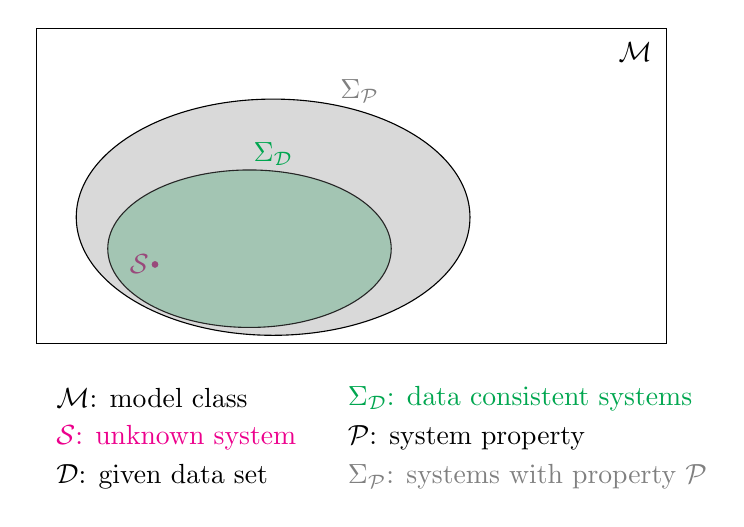
\begin{tikzpicture}[scale=1]
			\node[draw,rectangle,minimum width=8cm,minimum height = 4cm] (1) at (0,0) {};
			\node[] (2) at (3.6,1.7) {$\mathcal{M}$};
			\node[draw,fill,style=circle,inner sep=0pt,minimum size=2pt,color=magenta] (3) at (-2.5,-1) {};
			\node[color=magenta] (4) at (-2.7,-1) {$\mathcal{S}$};
			\node[label=right:{$\mathcal{M}$: model class}] at (-4,-2.7) {};
			\node[label=right:{\magenta{$\mathcal{S}$: unknown system}}] at (-4,-3.2) {};
			\node[label=right:{$\mathcal{D}$: given data set}] at (-4,-3.7) {};
			\node[label=right:{\green{$\Sigma_\mathcal{D}$: data consistent systems}}] at (-0.3,-2.7) {};
			\node[label=right:{\gray{$\Sigma_\mathcal{P}$: systems with property $\calP$}}] at (-0.3,-3.7) {};
			\node[label=right:{$\mathcal{P}$: system property}] at (-0.3,-3.2) {};
			\draw [fill=greenpigment,fill opacity=0.3] (-1.3,-0.8) ellipse (1.8cm and 1cm);
			\draw [fill=gray,fill opacity=0.3] (-1,-0.4) ellipse (2.5cm and 1.5cm);
			\node[] at (-1,.4) {\green{$\Sigma_\mathcal{D}$}};
			\node[] at (0.1,1.2) {\gray{$\Sigma_\mathcal{P}$}};
			%{$\mathcal{P}$}
		\end{tikzpicture}
		\caption{\cite{vanwaarde2023informativity}, Data is informative for property}
		\label{fig:informativedata}
\end{figure}	
\begin{figure}[h!]
		\centering
			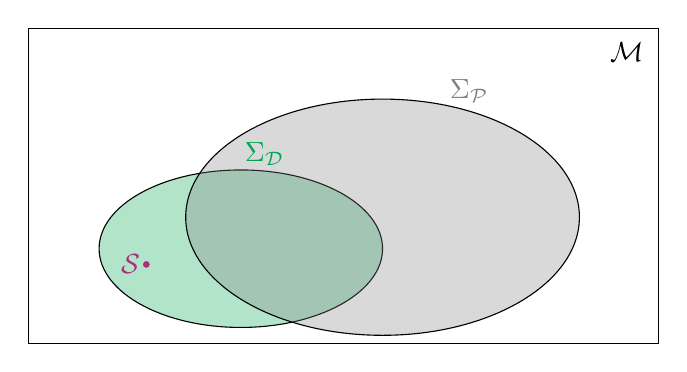
\begin{tikzpicture}[scale=1]
			\node[draw,rectangle,minimum width=8cm,minimum height = 4cm] (1) at (0,0) {};
			\node[] (2) at (3.6,1.7) {$\mathcal{M}$};
			\node[draw,fill,style=circle,inner sep=0pt,minimum size=2pt,color=magenta] (3) at (-2.5,-1) {};
			\node[color=magenta] (4) at (-2.7,-1) {$\mathcal{S}$};
			\draw [fill=greenpigment,fill opacity=0.3] (-1.3,-0.8) ellipse (1.8cm and 1cm);
			\draw [fill=gray,fill opacity=0.3] (0.5,-0.4) ellipse (2.5cm and 1.5cm);
			\node[] at (-1,.4) {\green{$\Sigma_\mathcal{D}$}};
			\node[] at (1.6,1.2) {\gray{$\Sigma_\mathcal{P}$}};
			%{$\mathcal{P}$}
		\end{tikzpicture}
		\caption{\cite{vanwaarde2023informativity}, Data is not informative for property}
		\label{fig:notinformativedata}
\end{figure}
\begin{definition}[\cite{vanwaarde2023informativity}, Informativity for analysis]\label{ch1:def:informativity}
	The data $\calD$ is \textit{informative} for property $\calP$ if $\Sigma_\calD \subseteq\Sigma_\calP$.
\end{definition}	
\begin{problem}[\cite{vanwaarde2023informativity}, Informativity problem for analysis]\label{ch3:prob:general}
	Provide necessary and sufficient conditions on the data $\calD$ under which these data are informative for property $\calP$. 
\end{problem}
\subsection{Incorporating Control problems}
Consider the problem of designing a controller $\calK$ meeting a desired control objective $\cal{O}$ for a data-driven control problem. Let $\Sigma_{\calO}$ be the set of all systems satisfying the control objective $\calO$ and $\Sigma_{\calD}(\calK)$ are all systems obtained by interconnecting the systems in $\Sigma_{\calD}$ with the controller. This give rise to the following informativity problem.
% For the framework to allow for data-driven control problems, we will consider a given control objective 
% $\cal{O}$.  Denote by  the set of all systems that satisfy the control objective $\calO$. For a given controller $\calK$, denote by $\Sigma_{\calD}(\calK)$ the set of all systems obtained as the interconnection of a system in $\Sigma_{\calD}$ with the controller $\calK$. We then have the following variant of informativity:
\begin{definition}[\cite{vanwaarde2023informativity}, Informativity for control]\label{ch1:def:par informativity}
The data $\calD$ is \textit{informative} for the control objective $\calO$ if there exists a controller $\calK$ such that $\Sigma_{\calD}(\calK) \subseteq \Sigma_{\calO}$. 
\end{definition}
And the two problems associated with this informativity is to first determine if such controller exists and then to design the controller.
% Obviously, the first step in any data-driven control problem is to determine whether it is possible to obtain, from the given data, a suitable controller. This leads to the following informativity problem:
\begin{problem}[\cite{vanwaarde2023informativity}, Informativity problem for control]\label{ch1:prob:parametrized}
Provide necessary and sufficient conditions on $\calD$ under which the data are informative for the control objective $\calO$. 
\end{problem}
% The second step of data-driven control involves the design of a suitable controller. In terms of our framework, this can be stated as:
\begin{problem}[\cite{vanwaarde2023informativity}, Control design problem]\label{ch1:prob:design}
	Assuming the data $\calD$ is informative for the control objective $\calO$, find a controller $\calK$ such that $\Sigma_\calD (\calK) \subseteq \Sigma_{\calO}$. 
\end{problem}
% The data-driven control design problem as formulated here has a rather natural interpretation as a problem of robust control. Indeed, the aim is to find one single controller that achieves the design objective for all systems  that are consistent with the data. In other words, the `system uncertainty` is determined directly by the given data, and no attempt is made to identify in any sense an uncertainty description that is suitable for existing methods in robust control design. The given data are called informative for a given design objective if the associated robust control problem allows a solution for the system uncertainty imposed by the data.

This framework is already used for various control problems taking two main directions, based on exact data (`E') and noisy (`N') data and based on data requirements such as the need of input (`I'), output (`O') and state (`S') data.
Table~\ref{tab:summary} provides an summary of the available results and their data requirements.

% The data informativity framework has already been applied to various analysis and design problems. Generally speaking, there is a dichotomy between two main directions. On the one hand there are analysis and design problems based on exact, i.e., noiseless data. On the other hand we consider the more realistic situation that the data are noisy, in the sense that they are obtained from a true, unknown, system that is corrupted by additive noise. 

% The first column of the table states the considered system property or control design problem. The second column refers to the type of data that are used (for discrete-time systems). Here, `E' refers to exact data, and `N' to noisy data. State, input-state, input-state-output and input-output are denoted by `S', `IS', `ISO' and `IO', respectively.
% The results in the table apply to , and most of the results are for linear time-invariant dynamics.
\begin{table}[H]  
\begin{center}
{\small\begin{tabular}{l|c}
Problem & Data\\
\hline
{controllability} & E-IS\\
observability & E-S\\
{stabilizability} & E-IS, N-IS\\
stability & E-S, N-S, N-IO\\
{LQR} & E-IS\\
{dissipativity} & E-ISO, N-ISO\\
{tracking and regulation} & E-IS\\
\end{tabular}}
\end{center}
\caption{\cite{vanwaarde2023informativity}, Summary of results}
\label{tab:summary}
\end{table}
Initially we will review select analysis and design problems and then proceed to describe a new approach based on current literature.
% The purpose of this paper is to highlight the strength of the informativity framework by reviewing a selection of analysis and design problems, indicated in Table~\ref{tab:summary} in red. Both exact and noisy data will be discussed in the present paper.

% This paper is divided into three main sections. These sections are divided into subsections, each devoted to a particular analysis or control design problem. In the first main section our model class will be chosen as the set of all discrete-time linear input-state systems with given state and input dimensions. The data are measurements of the state and input obtained from a true, unknown, system on a given finite time-interval. In this first section it is assumed that the data are noiseless, in the sense that the true system does not contain any noise input. In this noiseless framework we discuss the problem of informativity for the system properties controllability and stabilizability. Next, as a first control design problem we discuss the problem of stabilization by static state feedback, and take a look at the corresponding informativity problem. In the third subsection we study informativity in the context of the linear quadratic regulator problem, and, finally, in the fourth subsection we look at the classical problem of tracking and regulation. 

% In the second main section we incorporate noise into the models and data. The model class consists of all input-state systems with additive noise and the input-state data are assumed to be obtained from the noisy true system. The additive noise is unknown, but its samples on the data sampling interval are assumed to satisfy a given quadratic matrix inequality. In this framework we discuss a number of analysis and control design problems. In the first subsection we again look at the problem of stabilization by state feedback, this time in a noisy setting. The next subsection deal with informativity in the context of the well known ${\calH}_{\infty}$ control problem. The final subsection of this part deals with the problem of determining from noisy data whether an unknown system is dissipative with respect to a given supply rate.
\section{Informativity for analysis (Controllability and Stabilizability)}
% Recall from Definition~\ref{ch1:def:informativity} the definition of informativity of data for a given system property. In accordance with Definition~\ref{ch1:def:informativity} we say that the data $(U_-,X)$ are {\em informative for controllability} if all systems in $\Sigma_\calD$ are controllable. Likewise, we call the data  {\em informative for stabilizability} if all systems in $\Sigma_\calD$ are stabilizable.
The informativity notion is straightforward from the definition~\ref{ch1:def:informativity}. Given data is {\em informative for controllability (stabilizability)} if all systems in $\Sigma_\calD$ are controllable (stabilizable).

So, let's focus on the informativity problem for analysis which can be solved using the following theorem.
\begin{theorem}[\cite{vanwaarde2023informativity}, Data-driven Hautus tests]
	\label{ch2:t:contstab}
	The data $(U_-,X)$ is informative for controllability (stabilizability) if and only if 
	\begin{equation}
		\label{ch2:eq:rank for cont}
		\rank ( X_+ -\lambda X_-) = n \quad \forall \lambda \in \mathbb{C} \quad (\textrm{with } |\lambda|\geq 1).
	\end{equation}
	% Similarly, the data $(U_-,X)$ are informative for  if and only if 
	% \begin{equation}\label{ch2:eq:rank for stab}
	% 	\rank ( X_+ -\lambda X_-) = n \quad \forall \lambda \in \mathbb{C}\textrm{ with } |\lambda|\geq 1.
	% \end{equation}
\end{theorem}
This also shows that the rank condition \eqref{ch2:eq:inf for sys ident} is not necessary for data-driven analysis.
% Note that condition \eqref{ch2:eq:inf for sys ident} is not necessary to perform data-driven analysis in general. There are situations in which we can conclude controllability or stabilizability from the data without being able to identify the true system uniquely. This can be seen by the fact that in order for \eqref{ch2:eq:inf for sys ident} to hold we require at least $m+n$ separate measurements, whereas the conditions of Theorem~\ref{ch2:t:contstab} can hold for $n$ measurements. This is illustrated in the following example.

\begin{comment}
	\begin{exm}[Full rank is not necessary]
		Suppose that $n=2$ and $m=1$. Assume we collect data on the single time interval $\{0,1 \ldots, T\}$ with $T = 2$ to obtain
		\[ X= \begin{bmatrix} 0 & 1 & 0 \\ 0 & 0 & 1 \end{bmatrix} \textrm{ and } U_-= \begin{bmatrix} 1 & 0 \end{bmatrix}. \] 
		This implies that 
		\[X_+ = \begin{bmatrix} 1 & 0 \\ 0 & 1 \end{bmatrix} \textrm{ and } X_- = \begin{bmatrix} 0 & 1 \\ 0& 0\end{bmatrix}. \]
		Using Theorem~\ref{ch2:t:contstab} we see that these data are informative for controllability, as 
		\[ \rank \begin{bmatrix} 1 & -\lambda \\ 0 & 1 \end{bmatrix}= 2 \quad \forall \lambda \in \mathbb{C}.\] 
		Recall that this means that all systems consistent with the data are controllable. Therefore we can conclude that also the true system is controllable. Moreover, note that the rank condition \eqref{ch2:eq:inf for sys ident} does not hold, and therefore $\Sigma_\calD$ is not a singleton.  To be precise:
		\begin{equation}\label{ch2:eq:structural} \Sigma_\calD = \left\lbrace \left( \begin{bmatrix} 0 & a_1 \\ 1 & a_2\end{bmatrix} ,\begin{bmatrix} 1 \\ 0 \end{bmatrix}\right) \mid a_1,a_2 \in\mathbb{R} \right\rbrace.
		\end{equation}
		This means that there are multiple systems consistent with the data.
	\end{exm}
\end{comment}
% Computationally, the conditions \eqref{ch2:eq:rank for cont} and \eqref{ch2:eq:rank for stab} might seem daunting, since these require to test the rank of a matrix for each $\lambda\in\mathbb{C}$. However, it is well known that in order for the classical Hautus test to be satisfied, it suffices to test the rank for only $\lambda\in \sigma(A)$, where $\sigma(A)$ denotes the set of eigenvalues of the matrix $A$. 
\begin{comment}
	
	In a similar fashion, the conditions of Theorem~\ref{ch2:t:contstab} can be verified in a finite number of steps. Indeed, \eqref{ch2:eq:rank for cont} is equivalent to 
	\[ \rank(X_+)=n \textrm{ and } \rank ( X_+ -\lambda X_-) = n \]
	for all $\lambda\neq 0$ with $\lambda\inv\in\sigma(X_-X_+^\sharp)$, where $X_+^\sharp$ is any right inverse of $X_+$. Regarding stabilizability, we obtain that \eqref{ch2:eq:rank for stab} is equivalent to 
	\[\rank(X_+-X_-)=n \textrm { and } \rank ( X_+ -\lambda X_-) = n \]
	for all $\lambda\neq 1$ with $(\lambda-1)\inv\in\sigma(X_-(X_+-X_-)^\sharp)$.

	%\begin{remark}[Comparing this to the other results on controllability]
	%	- Harry/Jaap paper? The paper(s) by Liu? 
	%\end{remark}
\end{comment}
% After considering data-driven controllability and stabilizability analysis in the previous subsection, we now turn attention to data-driven control design. In particular, we consider the quintessential control problem of stabilization by state feedback. 
\section{Informativity for control (Stabilization)}
\label{sec:stability informativity}
Usingn~\ref{ch1:def:par informativity}. 
We define our sets as follows,
% We take the model class $\calM$ and data $\calD$ as before, and take as the control objective $\calO$: `interconnection with a  state feedback controller yields a stable\footnote{meaning Schur, that is, all its eigenvalues $\lambda$ satisfy $\abs{\lambda}<1$.}, closed loop system'. This means that the set $\Sigma_{\calO}$ of all systems that satisfy the control objective is equal to the set of all stable $n \times n$ matrices
$$
\Sigma_{\calO} :=  \{ A \in \R^{n \times n} \mid A \text{ is stable} \} \qquad\text{and}\qquad \Sigma_\calD(K) = \{ A+ BK \mid (A,B) \in \Sigma_\calD \}. 
$$

As per \ref{ch1:def:par informativity}, data $(U_-,X)$ is {\em informative for stabilization by state feedback} if there exists a $K \in \mathbb{R}^{m \times n}$ such that $\Sigma_\calD(K) \subseteq \Sigma_{\calO}$.

% In other words, the input-state data $(U_-,X)$ are informative for stabilization by state feedback if there exists a single real $m \times n$ matrix $K$ such that $A +BK$ is stable for all $(A,B) \in \calM$ that are consistent with the data.

%\begin{remark} 
% At this point, one may wonder about the relation between informativity for stabilizability and informativity for stabilization. It is clear that the data $(U_-,X)$ are informative for stabilizability if $(U_-,X)$ are informative for stabilization by state feedback. However, the reverse statement does not hold in general. This is due to the fact that all systems $(A,B)$ in $\Sigma_\calD$ may be stabilizable, but there may not exist a \emph{common} feedback gain $K$ such that $A+BK$ is stable for all of these systems. 
%\end{remark}
\begin{comment}
	
	The following example further illustrates the difference between informativity for stabilizability and informativity for stabilization.

	\begin{exm}[Stabilizability and stabilization]
		Consider the scalar system 
		$
		\bmx(t+1)= \bmu(t),
		$
		where $\bmx, \bmu \in \mathbb{R}$. Suppose that we collect data on the single time interval $\{0,1\}$, specifically, $x(0) = 0$, $u(0) = 1$ and $x(1) = 1$. This means that $U_- = \begin{bmatrix}1 \end{bmatrix}$ and $X = \begin{bmatrix}0 & 1	\end{bmatrix}$. It can be shown that $\Sigma_\calD = \{(a,1) \mid a \in \mathbb{R}\}$. Clearly, all systems in $\Sigma_\calD$ are stabilizable. Nonetheless, the data are not informative for \emph{stabilization}. This is because the systems $(-1,1)$ and $(1,1)$ in $\Sigma_\calD$ cannot be stabilized by the \emph{same} controller of the form $u(t) = K x(t)$. 
		We conclude that informativity of the data for stabilizability does not imply informativity for stabilization by state feedback. 
	\end{exm}

	Having defined the notion of informativity for stabilization, we now take the steps described in the introduction. First, we resolve Problem~\ref{ch1:prob:parametrized}, that is, we find necessary and sufficient conditions for informativity for stabilization by state feedback. After this, we design a corresponding controller, as described in Problem~\ref{ch1:prob:design}. 

\end{comment}
To solve the problem, consider the solution set of the homogeneous equation which will allow the to deduce the membership of $A,B$ in $\Sigma_{\calD}$
\begin{equation}\label{ch3:eq:sigma is 0}
	\Sigma_\calD^0 := \left\{(A_0,B_0) \mid 0 = \bbm A_0 & B_0 \ebm
	\begin{bmatrix}
		X_- \\ U_-
	\end{bmatrix}\right\}.
\end{equation}
We first state a useful lemma using the fact that $(A,B)\in\Sigma_\calD$ if and only if it is a solution of the the corresponding affine equation. Now let $\Sigma_\calD^0$ denote the solution set of the corresponding homogeneous equation. That is, 
% This allows us to state the following lemma. 
\begin{lemma}[\cite{vanwaarde2023informativity}, A necessary condition]
	\label{ch3:lemmaF0=0}
	If the data $(U_-,X)$ is informative for stabilization by state feedback then $A_0 + B_0 K = 0$ for all $(A_0,B_0) \in \Sigma_\calD^0$. Equivalently, 
	$$
	\im \begin{bmatrix}
		I \\ K
	\end{bmatrix} \subseteq 
	\im \begin{bmatrix}
		X_- \\ U_-
	\end{bmatrix}.
	$$
\end{lemma}

% The solution set of an affine equation is equal to the sum of any solution and the solution set of the corresponding homogenous equation. Since we know that $(A_s,B_s)\in\Sigma_\calD$ by definition, this means that we can write 
% \[ \Sigma_\calD = (A_s,B_s) + \Sigma_\calD^0.\]
% Using this, as a consequence of Lemma~\ref{ch3:lemmaF0=0} we have that if $K$ is a  feedback gain such that $A+BK$ is stable for all $(A,B) \in \Sigma_\calD$, then
% \[ \Sigma_\calD(K) = \{A_s+B_sK\},  \] 
% that is, the set of closed-loop systems consistent with the data is a singleton. It is important to note, however, that this does not mean that $\Sigma_\calD$ is necessarily a singleton.

% The above observation turns out to be instrumental in proving the following theorem, which gives necessary and sufficient conditions for informativity for stabilization by state feedback. 

This observations helps us to solve the problem of informativity for stabilization.
\begin{theorem}[\cite{vanwaarde2023informativity}, Conditions for stabilization]
	\label{ch3:t:algstab}
	The data $(U_-,X)$ is informative for stabilization by state feedback if and only if the matrix $X_-$ has full row rank and there exists a right inverse $X_-^\sharp$ of $X_-$ such that $X_+ X_-^\sharp$ is stable. 
	
	Moreover, $K$ is such that $A +BK$ is stable for all $(A,B) \in \Sigma_\calD$ if and only if $K = U_- X_-^\sharp$.
	% , where $X_-^\sharp$ satisfies the above properties.
	% In that case, $A +BK = X_+ X_-^\sharp$ for all $(A,B) \in \Sigma_\calD$.
\end{theorem}
The above theorem though is not constructive as it does not provide the means to calculate such right inverse of $X_-$. To resolve this, the following LMI-based approach is utilised.
% Theorem \ref{ch3:t:algstab} gives a characterization of all input-state data that are informative for stabilization by state feedback and provides a stabilizing controller. Nonetheless, the procedure to compute this controller might not be entirely satisfactory since it is not clear how to find a right inverse of $X_-$ that makes $X_+ X_-^\sharp$ stable. In general, $X_-$ has many right inverses, and $X_+ X_-^\sharp$ can be stable or unstable depending on the particular right inverse $X_-^\sharp$. To deal with this problem and to solve the design problem, we give a characterization of informativity for stabilization in terms of linear matrix inequalities (LMIs). The feasibility of such LMIs can be verified using standard tools. 
\begin{theorem}[\cite{vanwaarde2023informativity}, LMI conditions for stabilization]\label{ch3:t:lmistab}
	The data $(U_-,X)$ are informative for stabilization by state feedback if and only if there exists a matrix $\Theta \in \mathbb{R}^{T \times n}$ satisfying
	\begin{equation}
		\label{ch3:LMI/E}
		X_- \Theta = (X_- \Theta)^\top\quad\text{ and }\quad
		\begin{bmatrix}
			X_- \Theta & X_+ \Theta \\ \Theta^\top X_+^\top & X_- \Theta
		\end{bmatrix} > 0.
	\end{equation}
	Moreover, $K$ is such that $A +BK$ is stable for all $(A,B) \in \Sigma_\calD$ if and only if $K = U_- \Theta (X_-\Theta)^{-1}$ for some matrix $\Theta$ satisfying \eqref{ch3:LMI/E}.
\end{theorem}
\begin{comment}
	
	The following example provides a simple illustration of the above results. 
	\begin{exm}[Full rank not necessary for informativity] 
		Consider an unstable system $(A_s,B_s)$, where $A_s$ and $B_s$ are given by
		$$
		A_s = \begin{bmatrix}
			1.5 & 0 \\ 1 & 0.5
		\end{bmatrix}, \quad B_s = \begin{bmatrix}
			1 \\ 0
		\end{bmatrix}.
		$$
		We collect data from this system on a single time interval from $t = 0$ until $t = 2$, which results in the data matrices
		$$
		X = \begin{bmatrix}
			1 & 0.5 & -0.25 \\
			0 & 1 & 1
		\end{bmatrix}, \quad U_- = \begin{bmatrix}
			-1 & -1
		\end{bmatrix}.
		$$
		Clearly, the matrix $X_-$ is square and invertible, and it can be verified that
		$$
		X_+ X_-^{-1} = \begin{bmatrix}
			0.5 & -0.5 \\
			1 & 0.5
		\end{bmatrix}
		$$
		is stable, since its eigenvalues are $\half(1 \pm \sqrt{2}i)$. We conclude by Theorem \ref{ch3:t:algstab} that the data $(U_-,X)$ are informative for stabilization by state feedback. The same conclusion can be drawn from Theorem \ref{ch3:t:lmistab} since $$\Theta = \begin{bmatrix}
			1 & -1 \\ 0 & 2
		\end{bmatrix}$$ solves \eqref{ch3:LMI/E}. Next, we can conclude from either Theorem \ref{ch3:t:algstab} or Theorem \ref{ch3:t:lmistab} that the stabilizing feedback gain in this example is unique, and given by $K = U_-X_-^{-1} = \begin{bmatrix}
			-1 & -0.5
		\end{bmatrix}$. Finally, it is worth noting that the data are not informative for identification. In fact, $(A,B) \in \Sigma_\calD$ if and only if
		$$
		A = \begin{bmatrix}
			1.5+a_1 & 0.5a_1 \\ 1+ a_2 & 0.5+ 0.5a_2
		\end{bmatrix}, \quad B = \begin{bmatrix}
			1+a_1 \\ a_2
		\end{bmatrix}
		$$
		for some $a_1$ and $a_2 \in \mathbb{R}$.
	\end{exm}
\end{comment}
%
%
%\section{Analysis and control using exact input-state data}
%
%In order to provide a solid foundation for more complex problems, in this section we will first consider the essential model class of linear, time-invariant input-state systems. Our goal is to analyze and control these systems on the basis of input-state data, consisting of a finite number of measurements of the input and state trajectories. Moreover, we will assume that these measurements are exact, that is, not corrupted by any noise. 
%
%Given this situation, we can make the abstract framework that was introduced in the introduction more tangible. To be precise, the unknown system $\calS$ is assumed to be the following:
%\begin{equation} \label{ch2:eq:true system once more}
%	\bmx(t+1) = A_s\bmx(t) + B_s\bmu(t),
%\end{equation}
%where $\bmx$ denotes the $n$-dimensional state and $\bmu$ the $m$-dimensional input. In the following, we assume that the dimensions $n$ and $m$ are known, but the matrices $A_s$ and $B_s$ are unknown. As such, we see that $\calS$ is contained in the model class $\calM$ given by the set of all discrete-time linear input-state systems of the form
%\begin{equation}  \label{ch2:e: is-system}
%	\bmx(t+1) = A\bmx(t) + B\bmu(t),
%\end{equation}
%with given state space and input dimensions $n$ and $m$. 
%
%Suppose that we collect input-state data from the true system \eqref{ch2:eq:true system once more} on $\ell$ time intervals $\pset{0,1,\ldots,T_i}$ for $i=1,2,\ldots,\ell$, in the sense that we excite the true system with input sequences $u^i(0)$, $u^i(1)$, $\ldots$, $u^i(T_i-1)$ and obtain measurements of corresponding state sequences $x^i(0)$, $x^i(1)$, $\ldots$, $x^i(T_i)$. We can collect these measurements in matrices by defining for each $i$:
%\begin{subequations}\label{ch2:eq: UXdata}
%	\begin{align}
%		U^i_-& := \bbm u^i(0) & u^i(1) & \cdots & u^i(T_i-1)\ebm, \\
%		X^i& := \bbm x^i(0) & x^i(1) & \cdots & x^i(T_i)\ebm. \label{ch2:eq: UXdata2}
%	\end{align}
%\end{subequations}
%If, additionally, we define the matrices
%\begin{subequations}\label{ch2:eq: def of X- X+}
%	\begin{align}
%		X^i_-& := \bbm x^i(0) & x^i(1) & \cdots & x^i(T_i-1) \ebm, \\
%		X^i_+& := \bbm x^i(1) & x^i(2) & \cdots & x^i(T_i) \ebm,
%	\end{align}	
%\end{subequations}
%we have $X^i_+=A_sX^i_-+B_sU^i_-$ for each $i$, since the data were assumed to be generated by the true system. In a similar fashion, we can arrange these matrices corresponding to separate intervals in the following manner:
%\bse\label{ch2:eq: UXdatanew}
%\begin{alignat}{3}
%	U_-&:=\bbm U^1_-&\cdots& U^\ell_-\ebm,&\quad X&:=\bbm X^1&\cdots& X^\ell\ebm,\label{ch2:eq: UXdatanew1}\\
%	X_-&:=\bbm X^1_-&\cdots& X^\ell_-\ebm,&\quad X_+&:=\bbm X^1_+&\cdots& X^\ell_+\ebm,\label{ch2:eq: UXdatanew2}
%\end{alignat}
%\ese
%As before, it is straightforward to check that $X_+=A_sX_-+B_sU_-$. Moreover, this is \textit{all} the information we have regarding the true system on the basis of the data $\calD:=(U_-,X)$. As explained in the introduction, we are interested in the set $\Sigma_\calD$ containing all systems in $\calM$ that are consistent with these data. This means that the set $\Sigma_\calD$ is equal to $\Sigma_{(U_-,X)}$, defined by 
%\begin{equation}\label{ch2:eq:SigmaD}
%	\Sigma_{(U_-,X)} := \left\{ (A,B) \in \calM \mid X_+= \bbm A&B \ebm
%	\begin{bmatrix}
%		X_-\\U_-
%	\end{bmatrix} \right\}. 
%\end{equation}
%
%Note that since $(A_s,B_s) \in \Sigma_{(U_-,X)}$, it is nonempty. Moreover it is the solution set of an affine equation. Therefore, it is a singleton if and only if 
%\begin{equation}\label{ch2:eq:inf for sys ident} \rank \begin{bmatrix} X_- \\ U_- \end{bmatrix} = n+m. \end{equation}
%
%Under this condition, we can find $\Sigma_{(U_-,X)}=\{(A_s,B_s)\}$, and then use a model-based method to check whether $(A_s,B_s)$ has a given property. 
%
%\begin{remark}[The fundamental lemma] 
%	In the previous, we have considered the situation where the measurements are given. A problem that is closely related to those considered in this paper is: Can we pick inputs $u(t)$, such that the resulting state trajectory is such that \eqref{ch2:eq:inf for sys ident} holds? The answer to this question can be  found using the notion of \textit{persistently exciting} inputs. 
%	
%	To be precise, consider the finite length sequence $u(0)$, $u(1)$, $\ldots$, $u(T-1)$. Denote the vector
%	\[ u_{[i,j]} = \begin{bmatrix} u(i)^\top \ldots u(j)^\top\end{bmatrix}^\top, \]
%	and define the Hankel matrix of depth $k$ by
%	
%	\[H_k(u_{[0,T-1]}) := \begin{bmatrix}
%		u(0) 	& u(1) 		& \cdots 	& u(T - k) \\
%		u(1) 	& u(2) 		& \cdots 	& u(T - k +1) \\
%		\vdots  & \vdots	&    		& \vdots  \\
%		u(k-1)  & u(k) 		& \cdots  	& u(T-1) 
%	\end{bmatrix}. \]
%	We say that the input sequence $u_{[0,T-1]}$ is \textit{persistently exciting} of order $k$ if $H_k(u_{[0,T-1]})$ has full row rank. 
%	
%	A special case of Willem's fundamental lemma \cite[Thm. 1]{vanWaarde2020c} (originally proven in a behavioral context in \cite[Thm. 1]{Willems2005}) states the following: Suppose that the measured system is controllable and that the input sequence is \textit{persistently exciting} of order $n+L$. Then any  $\bar{u}_{[0,L-1]},\bar{x}_{[0,L-1]}$ is an input/state trajectory of the system if and only if 
%	\[ \begin{bmatrix} \bar{u}_{[0,L-1]} \\ \bar{x}_{[0,L-1]} \end{bmatrix} \in \im \begin{bmatrix} H_L(u_{[0,T-1]}) \\ H_L(x_{[0,T-1]}) \end{bmatrix}. \] 
%	
%	As a consequence, we can guarantee that \eqref{ch2:eq:inf for sys ident} holds by assuming that $u_{[0,T-1]}$ is persistently exciting of degree $n+1$. Recall that, if the condition \eqref{ch2:eq:inf for sys ident} holds, we know that there exists a unique system in $\Sigma_{(U_-,X)}$. Once we have identified a model of this system, we can apply any number of model-based methods in order to, for instance, stabilize it. 
%	
%	However, in many applications a (state space) model might not be the most convenient form to work with. One of these applications is Data-enabled Predictive control (DeePC), introduced in \cite{Coulson2019}. As a data-driven variant of Model Predictive Control (MPC), the central problem is to minimize a cost function over all length-$L$ trajectories. The fundamental lemma allows this to be formulated in terms of measurements, without explicitly finding a system model.  
%	
%	On the other hand, there are many other applications where avoiding the modeling step, and dealing with data directly is convenient. For example, the paper \cite{DePersis2020} provides efficient methods for stabilization on the basis measurements for which \eqref{ch2:eq:inf for sys ident} holds. 	
%\end{remark}
%
%\subsection{Controllability and stabilizability}
%
%As we will show in this subsection, condition \eqref{ch2:eq:inf for sys ident} is not necessary to perform data-driven analysis in general. As an illustration, we will establish necessary and sufficient conditions in terms of the data for verifying controllability and stabilizability, which do not require the rank condition to hold.
%
%Recall from Definition~\ref{ch1:def:informativity} the definition of informativity of data for a given system property. In accordance with Definition~\ref{ch1:def:informativity} we say that the data $(U_-,X)$ are {\em informative for controllability} if all systems in $\Sigma_{(U_-,X)}$ are controllable. Likewise, we call the data  {\em informative for stabilizability} if all systems in $\Sigma_{(U_-,X)}$ are stabilizable.
%
%In order to establish tests for these notions of informativity, the well known Hautus test 
%%\cite[Thm. 3.13]{Trentelman2001} 
%for controllability can be used: a system $(A,B)$ is controllable if and only if
%\begin{equation}\label{ch2:eq:Hautus} \rank \begin{bmatrix} A-\lambda I & B \end{bmatrix} =n \end{equation} 
%for all $\lambda\in \mathbb{C}$. For stabilizability, the Hautus test requires that \eqref{ch2:eq:Hautus} holds for all $\lambda$ outside the open unit disc.
%
%%Now, introduce the following subsets of the model class $\calM$ of all systems of the form \eqref{ch2:e: is-system} with fixed dimensions $n$ and $m$:
%%\begin{align*}
%%\Sigma_{\text{cont}} &:= \{ (A,B) \mid (A,B) \text{ is controllable} \} \\
%%\Sigma_{\text{stab}} &:= \{ (A,B) \mid (A,B) \text{ is stabilizable} \}.
%%\end{align*} 
%
%The following theorem gives necessary and sufficient conditions on the input-state data to be informative for these two properties. The result provides tests on the given data matrices
%
%
%\begin{theorem}[Data-driven Hautus tests]
%	\label{ch2:t:contstab}
%	The data $(U_-,X)$ are informative for controllability if and only if 
%	\begin{equation}
%		\label{ch2:eq:rank for cont}
%		\rank ( X_+ -\lambda X_-) = n \quad \forall \lambda \in \mathbb{C}.
%	\end{equation}
%	Similarly, the data $(U_-,X)$ are informative for stabilizability if and only if 
%	\begin{equation}\label{ch2:eq:rank for stab}
%		\rank ( X_+ -\lambda X_-) = n \quad \forall \lambda \in \mathbb{C}\textrm{ with } |\lambda|\geq 1.
%	\end{equation}
%\end{theorem}
%
%As announced at the beginning of this section, there are situations in which we can conclude controllability/stabilizability from the data without being able to identify the true system uniquely. This can be seen by the fact that in order for \eqref{ch2:eq:inf for sys ident} to hold we require at least $m+n$ separate measurements, whereas the conditions of Theorem~\ref{ch2:t:contstab} can hold for $n$ measurements. This is illustrated in the following example.
%
%\begin{exm}
%	Suppose that $n=2$ and $m=1$. Assume we collect data on the single time interval $\{0,1 \ldots, T\}$ with $T = 2$ to obtain
%	\[ X= \begin{bmatrix} 0 & 1 & 0 \\ 0 & 0 & 1 \end{bmatrix} \textrm{ and } U_-= \begin{bmatrix} 1 & 0 \end{bmatrix}. \] 
%	This implies that 
%	\[X_+ = \begin{bmatrix} 1 & 0 \\ 0 & 1 \end{bmatrix} \textrm{ and } X_- = \begin{bmatrix} 0 & 1 \\ 0& 0\end{bmatrix}. \]
%	Using Theorem~\ref{ch2:t:contstab} we see that these data are informative for controllability, as 
%	\[ \rank \begin{bmatrix} 1 & -\lambda \\ 0 & 1 \end{bmatrix}= 2 \quad \forall \lambda \in \mathbb{C}.\] 
%	Recall that this means that all systems consistent with the data are controllable. Therefore we can conclude that also the true system is controllable. Moreover, note that the rank condition \eqref{ch2:eq:inf for sys ident} does not hold, and therefore $\Sigma_{(U_-,X)}$ is not a singleton.  To be precise:
%	\begin{equation}\label{ch2:eq:structural} \Sigma_{(U_-,X)} = \left\lbrace \left( \begin{bmatrix} 0 & a_1 \\ 1 & a_2\end{bmatrix} ,\begin{bmatrix} 1 \\ 0 \end{bmatrix}\right) \mid a_1,a_2 \in\mathbb{R} \right\rbrace.
%	\end{equation}
%	This means that there are multiple systems consistent with the data.
%\end{exm}
%
%Computationally, the conditions \eqref{ch2:eq:rank for cont} and \eqref{ch2:eq:rank for stab} might seem daunting, since these require to test the rank of a matrix for each $\lambda\in\mathbb{C}$. However, it is well known that in order for the classical Hautus test to be satisfied, it suffices to test the rank of \eqref{ch2:eq:Hautus} for only $\lambda\in \sigma(A)$, where $\sigma(A)$ denotes the set of eigenvalues of the matrix $A$. 
%
%In a similar fashion, the conditions of Theorem~\ref{ch2:t:contstab} can be verified in a finite number of steps. Indeed, \eqref{ch2:eq:rank for cont} is equivalent to 
%\[ \rank(X_+)=n \textrm{ and } \rank ( X_+ -\lambda X_-) = n \]
%for all $\lambda\neq 0$ with $\lambda\inv\in\sigma(X_-X_+^\sharp)$, where $X_+^\sharp$ is any right inverse of $X_+$. Regarding stabilizability, we obtain that \eqref{ch2:eq:rank for stab} is equivalent to 
%\[\rank(X_+-X_-)=n \textrm { and } \rank ( X_+ -\lambda X_-) = n \]
%for all $\lambda\neq 1$ with $(\lambda-1)\inv\in\sigma(X_-(X_+-X_-)^\sharp)$.
%
%%\begin{remark}[Comparing this to the other results on controllability]
%%	- Harry/Jaap paper? The paper(s) by Liu? 
%%\end{remark}
%
%
%\subsection{Stabilization}
%After considering data-driven controllability and stabilizability analysis in the previous subsection, we now turn attention to data-driven control design. In particular, we consider the quintessential control problem of stabilization by state feedback. 
%
%Recall the definition of informativity for control as given in Definition~\ref{ch1:def:par informativity}. We take the model class $\calM$ and data $\calD$ as before, and take as the control objective $\calO$: `interconnection with a  state feedback controller yields a stable closed loop system'. This means that the set $\Sigma_{\calO}$ of all systems that satisfy the control objective is equal to the set of all stable $n \times n$ matrices
%$$
%M^{n \times n}_{\rm stab}:=  \{ A \in \R^{n \times n} \mid A \text{ is stable} \}.
%$$
%For a given state feedback controller $K\in\mathbb{R}^{m\times n}$, the corresponding set of closed loop systems consistent with the data is equal to 
%\[ 
%\Sigma_{(U_-,X)}(K) = \{ A+ BK \mid (A,B) \in \Sigma_{(U_-,X)} \}. 
%\] 
%In line with Definition \ref{ch1:def:par informativity} we say that the data $(U_-,X)$ are {\em informative for stabilization by state feedback} if there exists a $K \in \mathbb{R}^{m \times n}$ such that $\Sigma_{(U_-,X)}(K) \subseteq M^{n \times n}_{\rm stab}$.
%
%In other words, the input-state data $(U_-,X)$ are informative for stabilization by state feedback if there exists a single real $m \times n$ matrix $K$ such that $A +BK$ is stable for all $(A,B) \in \calM$ that are consistent with the data.
%
%%\begin{remark} 
%At this point, one may wonder about the relation between informativity for stabilizability and informativity for stabilization. It is clear that the data $(U_-,X)$ are informative for stabilizability if $(U_-,X)$ are informative for stabilization by state feedback. However, the reverse statement does not hold in general. This is due to the fact that all systems $(A,B)$ in $\Sigma_{(U_-,X)}$ may be stabilizable, but there may not exist a \emph{common} feedback gain $K$ such that $A+BK$ is stable for all of these systems. 
%%\end{remark}
%
%The following example further illustrates the difference between informativity for stabilizability and informativity for stabilization.
%
%\begin{exm}
%	Consider the scalar system 
%	$
%	\bmx(t+1)= \bmu(t),
%	$
%	where $\bmx, \bmu \in \mathbb{R}$. Suppose that we collect data on the single time interval $\{0,1\}$, specifically, $x(0) = 0$, $u(0) = 1$ and $x(1) = 1$. This means that $U_- = \begin{bmatrix}1 \end{bmatrix}$ and $X = \begin{bmatrix}0 & 1	\end{bmatrix}$. It can be shown that $\Sigma_{(U_-,X)} = \{(a,1) \mid a \in \mathbb{R}\}$. Clearly, all systems in $\Sigma_{(U_-,X)}$ are stabilizable. Nonetheless, the data are not informative for \emph{stabilization}. This is because the systems $(-1,1)$ and $(1,1)$ in $\Sigma_{(U_-,X)}$ cannot be stabilized by the \emph{same} controller of the form $u(t) = K x(t)$. 
%	We conclude that informativity of the data for stabilizability does not imply informativity for stabilization by state feedback. 
%\end{exm}
%
%Having defined the notion of informativity for stabilization, we now take the steps described in the introduction. First, we resolve Problem~\ref{ch1:prob:parametrized}, that is, we find necessary and sufficient conditions for informativity for stabilization by state feedback. After this, we design a corresponding controller, as described in Problem~\ref{ch1:prob:design}. 
%
%In order to do this, we first state a useful lemma. Recall from \eqref{ch2:eq:SigmaD} that $(A,B)\in\Sigma_{(U_-,X)}$ if and only if it is a solution of the the corresponding affine equation. Now let $\Sigma_{(U_-,X)}^0$ denote the solution set of the corresponding homogeneous equation. That is, \begin{equation}\label{ch3:eq:sigma is 0}
%	\Sigma_{(U_-,X)}^0 := \left\{(A_0,B_0) \mid 0 = \bbm A_0 & B_0 \ebm
%	\begin{bmatrix}
%		X_- \\ U_-
%	\end{bmatrix}\right\}.
%\end{equation}
%This allows us to state the following lemma. 
%\begin{lemma}
%	\label{ch3:lemmaF0=0}
%	Suppose that the data $(U_-,X)$ are informative for stabilization by state feedback, and let $K$ be a  feedback gain such that $A+BK$ is stable for all $(A,B) \in \Sigma_{(U_-,X)}$. Then $A_0 + B_0 K = 0$ for all $(A_0,B_0) \in \Sigma_{(U_-,X)}^0$. Equivalently, 
%	$$
%	\im \begin{bmatrix}
%		I \\ K
%	\end{bmatrix} \subseteq 
%	\im \begin{bmatrix}
%		X_- \\ U_-
%	\end{bmatrix}.
%	$$
%\end{lemma}
%
%The solution set of an affine equation is equal to the sum of any solution and the solution set of the corresponding homogenous equation. Since we know that $(A_s,B_s)\in\Sigma_{(U_-,X)}$ by definition, this means that we can write 
%\[ \Sigma_{(U_-,X)} = (A_s,B_s) + \Sigma_{(U_-,X)}^0.\]
%Using this, as a consequence of Lemma~\ref{ch3:lemmaF0=0} we have that if $K$ is a  feedback gain such that $A+BK$ is stable for all $(A,B) \in \Sigma_{(U_-,X)}$, then
%\[ \Sigma_{(U_-,X)}(K) = \{A_s+B_sK\},  \] 
%that is, the set of closed-loop systems consistent with the data is a singleton. It is important to note, however, that this does not mean that $\Sigma_{(U_-,X)}$ is necessarily a singleton.
%
%The above observation turns out to be instrumental in proving the following theorem, which gives necessary and sufficient conditions for informativity for stabilization by state feedback. 
%
%\begin{theorem}
%	\label{ch3:t:algstab}
%	The data $(U_-,X)$ are informative for stabilization by state feedback if and only if the matrix $X_-$ has full row rank and there exists a right inverse $X_-^\sharp$ of $X_-$ such that $X_+ X_-^\sharp$ is stable. 
%	
%	Moreover, $K$ is such that $A +BK$ is stable for all $(A,B) \in \Sigma_{(U_-,X)}$ if and only if $K = U_- X_-^\sharp$, where $X_-^\sharp$ satisfies the above properties. In that case, $A +BK = X_+ X_-^\sharp$ for all $(A,B) \in \Sigma_{(U_-,X)}$.
%\end{theorem}
%
%
%Theorem \ref{ch3:t:algstab} gives a characterization of all input-state data that are informative for stabilization by state feedback and provides a stabilizing controller. Nonetheless, the procedure to compute this controller might not be entirely satisfactory since it is not clear how to find a right inverse of $X_-$ that makes $X_+ X_-^\sharp$ stable. In general, $X_-$ has many right inverses, and $X_+ X_-^\sharp$ can be stable or unstable depending on the particular right inverse $X_-^\sharp$. To deal with this problem and to solve the design problem, we give a characterization of informativity for stabilization in terms of linear matrix inequalities (LMIs). The feasibility of such LMIs can be verified using standard tools. 
%
%\begin{theorem}\label{ch3:t:lmistab}
%	The data $(U_-,X)$ are informative for stabilization by state feedback if and only if there exists a matrix $\Theta \in \mathbb{R}^{T \times n}$ satisfying
%	\begin{equation}
%		\label{ch3:LMI/E}
%		X_- \Theta = (X_- \Theta)^\top\quad\text{ and }\quad
%		\begin{bmatrix}
%			X_- \Theta & X_+ \Theta \\ \Theta^\top X_+^\top & X_- \Theta
%		\end{bmatrix} > 0.
%	\end{equation}
%	Moreover, $K$ is such that $A +BK$ is stable for all $(A,B) \in \Sigma_{(U_-,X)}$ if and only if $K = U_- \Theta (X_-\Theta)^{-1}$ for some matrix $\Theta$ satisfying \eqref{ch3:LMI/E}.
%\end{theorem}
%
%\begin{remark}[Discussion on dd-stab]
%	--- Note work by others, e.g. Claudio. See commented text below. Note the work on sample complexity, where they essentially answer the question: Can we define $X_-,U_-$ with minimal $T$ for which the data are informative? Answer: yes, with $T=n$. https://arxiv.org/pdf/2203.00474.pdf
%%	To the best of our knowledge, LMI conditions for data-driven stabilization were first studied in \cite{DePersis2020}. In fact, the linear matrix inequality \eqref{ch3:LMI/E} is the same as that of \cite[Thm. 3]{DePersis2020}. However, an important difference is that the results in \cite{DePersis2020} assume that the input $ u $ is persistently exciting of sufficiently high order. In contrast, Theorem~\ref{ch3:t:lmistab}, as well as Theorem \ref{ch3:t:algstab}, do not require such conditions. The characterization \eqref{ch3:LMI/E} provides the minimal conditions on the data under which it is possible to obtain a stabilizing controller.
%\end{remark}
%
%The following example provides a simple illustration of the above results. 
%\begin{exm}
%	Consider an unstable system $(A_s,B_s)$, where $A_s$ and $B_s$ are given by
%	$$
%	A_s = \begin{bmatrix}
%		1.5 & 0 \\ 1 & 0.5
%	\end{bmatrix}, \quad B_s = \begin{bmatrix}
%		1 \\ 0
%	\end{bmatrix}.
%	$$
%	We collect data from this system on a single time interval from $t = 0$ until $t = 2$, which results in the data matrices
%	$$
%	X = \begin{bmatrix}
%		1 & 0.5 & -0.25 \\
%		0 & 1 & 1
%	\end{bmatrix}, \quad U_- = \begin{bmatrix}
%		-1 & -1
%	\end{bmatrix}.
%	$$
%	Clearly, the matrix $X_-$ is square and invertible, and it can be verified that
%	$$
%	X_+ X_-^{-1} = \begin{bmatrix}
%		0.5 & -0.5 \\
%		1 & 0.5
%	\end{bmatrix}
%	$$
%	is stable, since its eigenvalues are $\half(1 \pm \sqrt{2}i)$. We conclude by Theorem \ref{ch3:t:algstab} that the data $(U_-,X)$ are informative for stabilization by state feedback. The same conclusion can be drawn from Theorem \ref{ch3:t:lmistab} since $$\Theta = \begin{bmatrix}
%		1 & -1 \\ 0 & 2
%	\end{bmatrix}$$ solves \eqref{ch3:LMI/E}. Next, we can conclude from either Theorem \ref{ch3:t:algstab} or Theorem \ref{ch3:t:lmistab} that the stabilizing feedback gain in this example is unique, and given by $K = U_-X_-^{-1} = \begin{bmatrix}
%		-1 & -0.5
%	\end{bmatrix}$. Finally, it is worth noting that the data are not informative for system identification. In fact, $(A,B) \in \Sigma_{(U_-,X)}$ if and only if
%	$$
%	A = \begin{bmatrix}
%		1.5+a_1 & 0.5a_1 \\ 1+ a_2 & 0.5+ 0.5a_2
%	\end{bmatrix}, \quad B = \begin{bmatrix}
%		1+a_1 \\ a_2
%	\end{bmatrix}
%	$$
%	for some $a_1$ and $a_2 \in \mathbb{R}$.
%\end{exm}
%
\begin{comment}
	\section{The linear quadratic regulator problem}

	An important classical control design problem is the optimal linear quadratic regulator (LQR) problem. In this subsection we will study the data-driven version of this problem within the informativity framework.  

	For given state and input dimensions $n$ and $m$, again consider the model class $\mathcal{M}$ of all discrete-time linear input-state systems \eqref{ch2:e: is-system}.
	%\begin{equation} \label{ch4:e:discintext}
	%\bmx(t+1) = A\bmx(t) + B \bmu(t).
	%\end{equation}
	Consider the discrete time linear system 
	\begin{equation} \label{ch4:e:disc}
	\bmx(t+1) = A \bmx(t) + B \bmu(t),
	\end{equation}
	where $A$  and $B$ are matrices of dimensions $n \times n$ and $n \times m$, and where 
	$\bmx$ is the $n$-dimensional state and $\bmu$ the $m$-dimensional input. In the linear quadratic regulator problem we quantify the performance of the system using a quadratic cost functional $J(x_0,\bmu)$ involving the state trajectory $\bmx$ and the input $\bmu$. The optimal linear quadratic regulator problem is then the problem of finding, for each initial state $x_0$ of the system, an optimal input, i.e. an input that minimizes the cost functional. In this sidebar the basics of discrete-time linear quadratic optimal control are reviewed. In the sequel,  the abbreviation `LQR'  will be used for  `linear quadratic regulator'. 

	For an initial state $x_0$, let $\bmx_{x_0,\bmu}$ be the state sequence of \eqref{ch4:e:disc} resulting from the input $\bmu$ and initial condition $\bmx(0) = x_0$. We omit the subscript and simply write $\bmx$ whenever the dependence on $x_0$ and $\bmu$ is clear from the context. 

	Associated to system \eqref{ch4:e:disc}, we define the quadratic cost functional
	\begin{equation}\label{ch4:e:cost}
	J(x_0,\bmu)=\sum_{t=0}^\infty  \bmx^\top(t) Q \bmx(t) + \bmu^\top(t) R \bmu(t),
	\end{equation}
	where $Q \in \S{n}$ is positive semidefinite and $R \in \S{m}$ is positive definite. Then, the optimal LQR problem is the following: 
	\begin{problem}[The LQR problem]
		Determine for every initial condition $x_0$ an input $\bmu^*$, such that $\lim_{t\to\infty} \bmx_{x_0,\bmu^*}(t) = 0$, and the cost functional $J(x_0,\bmu)$ is minimized under this constraint. 
	\end{problem}
	\noindent Such an input $\bmu^*$ is called optimal for the given $x_0$. Of course, an optimal input does not necessarily exist for all $x_0$. We say that the optimal LQR problem is {\em solvable\/} for $(A,B,Q,R)$ if for every $x_0$ there exists an input ${\bmu}^*$ such that
	\begin{enumerate}
		\item The cost $J(x_0,\bmu^*)$ is finite.
		\item The limit $\lim_{t\to\infty}\bmx_{x_0,\bmu^*}(t)=0$. 
		\item The input $\bmu^*$ minimizes the cost functional, i.e., 
		\[J(x_0,{\bmu}^*)\leq J(x_0,\bar{\bmu})\]
		for all $\bar{\bmu}$ such that $\lim_{t\to\infty}\bmx_{x_0,\bar{\bmu}}(t)=0$.
	\end{enumerate}
	In the sequel, we will require the notion of observable eigenvalues. 
	%Recall from e.g. \cite[Sec. 3.5]{Trentelman2001} that 
	An eigenvalue $\lambda$ of $A$ is called $(Q,A)$-observable if 
	\[ 
	\rank \begin{bmatrix} A-\lambda I \\ Q \end{bmatrix}=n.
	\] 
	The following theorem provides necessary and sufficient conditions for the solvability of the optimal LQR problem for $(A,B,Q,R)$. 
	This theorem is the discrete-time analogue to the continuous-time case stated in \cite[Thm. 10.18]{Trentelman2001}. 
	\begin{theorem}[Conditions for LQR]\label{ch4:t:Harry}
		Let $Q \geq 0$ and $R >0$. Then the following statements hold:	
		\begin{enumerate}
			\item If $(A,B)$ is stabilizable, there exists a unique largest real symmetric solution $P^+$ to the discrete-time algebraic Riccati equation (DARE) 
			\begin{equation}
			\label{ch4:dare}
			P = A^\top PA-A^\top PB(R+B^\top P B)\inv B^\top  P A+Q,
			\end{equation}
			in the sense that $P^+ \geq P$ for every real symmetric $P$ satisfying \eqref{ch4:dare}. The matrix $P^+$ is positive semidefinite.
			\item If, in addition to stabilizability of $(A,B)$, every eigenvalue of $A$ on the unit circle is $(Q,A)$-observable then for every $x_0$ a unique optimal input $\bmu^*$ exists. Furthermore, this input sequence is generated by the feedback law $\bmu = K \bmx$, where
			\begin{equation}
			\label{ch4:optgain}
			K := -(R+B^\top P^+ B)\inv B^\top  P^+ A.
			\end{equation}
			Moreover, the matrix $A+BK$ is stable. 
			\item In fact, the optimal LQR problem is solvable for $(A,B,Q,R)$ if and only if $(A,B)$ is stabilizable and every eigenvalue of $A$ on the unit circle is $(Q,A)$-observable. 
		\end{enumerate}
	\end{theorem}

	If the optimal LQR problem is solvable for $(A,B,Q,R)$, we say that the matrix $K$ given by \eqref{ch4:optgain} is the optimal feedback gain for $(A,B,Q,R)$. 
	% section section_name (end)
	Assume we have input-state data on multiple time intervals, leading to data $\calD:= (U_-,X)$ as given in \eqref{ch2:eq: UXdata}. As before, the set $\Sigma_{\calD}$ of all systems in $\calM$ that are consistent with the data is then given by \eqref{ch2:eq:SigmaD}.
	%equal to 
	%	\begin{equation} 
	%	\label{ch4:eq: SigmaD}
	%	\Sigma_\calD = \left\{ (A,B) \in \calM\mid X_+= \bbm A&B \ebm
	%	\begin{bmatrix}
	%	X_-\\U_-
	%	\end{bmatrix} \right\}.
	%	\end{equation}
	We assume that the data are generated by the true (but unknown) system $(A_s,B_s)$, which is therefore in $\Sigma_\calD$ itself.

	In the context of the optimal LQR problem the control objective $\calO$ is: `the system must be  controlled using the optimal feedback gain'.  In order to formalize this, we introduce the following notation.
	For any given $K$, let $\Sigma^{Q,R}_{K}$ denote the set of all systems of the form \eqref{ch2:e: is-system} for which $K$ is the optimal feedback gain corresponding to $Q$ and $R$, that is,
	\[ 
	\Sigma_K^{Q,R}:=\set{(A,B) \in \calM }{K \text{ is optimal for }(A,B,Q,R)}.
	\]
	This gives rise to yet another notion of informativity in line with Definition~\ref{ch1:def:par informativity}. Indeed, informativity requires the existence of a single feedback gain that is optimal for all systems consistent with the data. For the definition of solvability of the optimal LQR problem we refer to the sidebar `The linear quadratic regulator problem`.
	\begin{definition}[Informativity for LQR]
		Given matrices $Q$ and $R$, we say that the data $\calD = (U_-,X)$ are \emph{informative for optimal linear quadratic regulation} if the optimal LQR problem is solvable for all $(A,B) \in \Sigma_{\calD} $ and there exists $K$ such that $\Sigma_{\calD} \subseteq \Sigma^{Q,R}_{K}$.
	\end{definition}
	An instrumental result in obtaining necessary and sufficient conditions for informativity for optimal linear quadratic regulation is the following lemma.
	\begin{lemma}[Common solution of the Riccati equation]\label{ch4:l: same P works for all}
	Let $Q=Q^\top$ be positive semidefinite and $R=R^\top$ be positive definite. Suppose the data $(U_-,X)$ are informative for optimal linear quadratic regulation. Let $K$ be such that $\Sigma_{\calD} \subseteq \Sigma^{Q,R}_{K}$. Then, there exist a square matrix $M$ and a positive semidefinite matrix $P^+$ such that for all $(A,B)\in\Sigma_{\calD}$
	\begin{align}
	&\!\!\!\!\!M=A+BK,\label{ch4:e: define M}\\
	&\!\!\!\!\!P^+\!= A^\top\! P^+\!A\! -\! A^\top\! P^+\!B(R + B^\top\! P^+\! B)\inv B^\top\!  P^+\! A + Q,\!\!\label{ch4:e:dare aux}\\
	&\!\!\!\!\!P^+-M^\top P^+M=K^\top RK+Q,\label{ch4:e:lyap aux}\\
	&\!\!\!\!\!K=-(R+B^\top P^+ B)\inv B^\top  P^+ A.\label{ch4:e:uni K aux}
	\end{align}
	\end{lemma}
	Statement \eqref{ch4:e:dare aux} of the lemma says that if the data are informative, there exists a common solution $P^+ \geq 0$ to the whole collection of AREs associated with systems $(A,B)$ that are consistent with the data. Statement \eqref{ch4:e:uni K aux} 
	says that if $K$ is the common optimal gain for all systems that are consistent with the data, then it must be of the expected form \eqref{ch4:e:uni K aux} for all  $(A,B)$ consistent with the data. According to \eqref{ch4:e: define M}, the optimal closed loop system matrices $A + BK$ are identical for all consistent pairs $(A,B)$.

	The following theorem gives necessary and sufficient conditions for informativity for optimal linear quadratic regulation. 
	\begin{theorem}[Conditions for informativity \cite{8960476}]\label{ch4:t:LQinform}
		Let $Q \geq 0$ and $R > 0$. Then the data $(U_-,X)$ are informative for optimal linear quadratic regulation if and only if at least one of the following two conditions hold:
		\begin{enumerate}
			\item\label{ch4:cond:a} The data $(U_-,X)$ are informative for identification, that is, $\Sigma_{\calD}=\pset{(A_s,B_s)}$, and the optimal LQR problem is solvable for $(A_s,B_s,Q,R)$. In this case, the optimal feedback gain $K$ is of the form \eqref{ch4:e:uni K aux} where $P^+$ is the largest real symmetric solution to \eqref{ch4:e:dare aux} with $A = A_s$ and $B = B_s$.
			\item\label{ch4:cond:b} For all $(A,B) \in \Sigma_{\calD}$ we have $A=A_s$. Moreover, $A_s$ is stable, $QA_s = 0$, and the optimal feedback gain is given by $K = 0$. 
		\end{enumerate}
	\end{theorem}

	This theorem should be interpreted as follows. Condition \ref{ch4:cond:b}) of Theorem \ref{ch4:t:LQinform} can be considered as a  pathological case in which the only $A$ consistent with the data is the true one, namely $A_s$. This matrix $A_s$ is stable and $QA_s = 0$. Since $\bmx(t) \in \im A_s$ for all $t > 0$, we have $Q \bmx(t) = 0$ for all $t > 0$ if the input function is chosen as $\bmu = 0$. Additionally, since $A_s$ is stable, this shows that the optimal input is equal to $\bmu^* = 0$. If we set aside the pathological case \ref{ch4:cond:b}), the main message of Theorem \ref{ch4:t:LQinform} is the following: if the data are informative for optimal linear quadratic regulation they are also informative for system identification, in the sense that the set of systems consistent with the data contains only one element, i.e., $\Sigma_{\calD} = \{(A_s,B_s) \}$. This observation is consistent with the paper \cite{Polderman1986} that showed the necessity of identifiability of the true system in adaptive LQ control.

	At first sight, this might seem like a negative result in the sense that data-driven LQR is only possible with data that are also informative enough to uniquely identify the system. However, at the same time, Theorem \ref{ch4:t:LQinform} can be viewed as a positive result in the sense that it provides fundamental justification for the data conditions imposed in e.g. \cite{DePersis2020}. Indeed, in \cite{DePersis2020} the data-driven infinite horizon LQR problem\footnote{Note that the authors of \cite{DePersis2020} formulate this problem as the minimization of the $H_2$-norm of a certain transfer matrix.} is solved using input-state data under the assumption that the input is persistently exciting of sufficiently high order. Under the latter assumption, the input-state data are informative for system identification, i.e., the matrices $A_s$ and $B_s$ can be uniquely determined from data. Theorem \ref{ch4:t:LQinform} justifies such a strong assumption on the richness of data in data-driven linear quadratic regulation.
	%
	%
	The data-driven \emph{finite} horizon LQR problem was solved under a persistency of excitation assumption in \cite{Markovsky2007}. Our results suggest that also in this case informativity for system identification is necessary for data-driven LQR, although further analysis is required to prove this claim.
	%\end{remark}

	Although Theorem \ref{ch4:t:LQinform} gives necessary and sufficient conditions under which the data are informative for optimal linear quadratic regulation, it might not be directly clear how these conditions can be verified given the input-state data. Therefore, in what follows we rephrase the conditions of Theorem \ref{ch4:t:LQinform} in terms of the data matrices $X$ and $U_-$.


	\begin{theorem}[Alternative conditions for informativity \cite{8960476}]
		\label{ch4:t:LQinform2}
		Let $Q \geq 0$ and $R >0$. Then the data $(U_-,X)$ are informative for optimal linear quadratic regulation if and only if at least one of the following two conditions hold:
		\begin{enumerate}
			\item\label{ch4:cond:a2} The data $(U_-,X)$ are informative for identification, equivalently, there exists $\begin{bmatrix} V_1 & V_2\end{bmatrix}$ such that 
	\begin{equation}\label{ch2:eq:V1 V2} \begin{bmatrix} X_- \\ U_- \end{bmatrix} \begin{bmatrix} 	V_1 & V_2	\end{bmatrix} = \begin{bmatrix} I_n & 0 \\ 0& I_m\end{bmatrix}. \end{equation}		
	Moreover, the optimal LQR problem is solvable for $(A_s,B_s,Q,R)$, where $A_s=X_+V_1$ and $B_s=X_+V_2$.
			\item\label{ch4:cond:b2} There exists $\Theta \in \mathbb{R}^{T \times n}$ such that $X_- \Theta = (X_- \Theta)^\top$, 	$U_- \Theta = 0 $, 
			\begin{equation}
			\label{ch4:e:LMI/E/K/Q}
			\begin{bmatrix}
			X_- \Theta & X_+ \Theta \\ \Theta^\top X_+^\top & X_- \Theta
			\end{bmatrix} > 0.
			\end{equation}
			and $ QX_+\Theta = 0$. 
		\end{enumerate}
	\end{theorem}

	It is also possible to directly compute the optimal LQR feedback gain $K$ from the given data. 
	%For this, we will employ ideas from the study of Riccati inequalities (see e.g \cite{Ran1988}).
	%The main idea is to replace the Riccati inequality by the linear matrix inequality $\mathcal{L}(P) \leq 0$, where
	%\begin{equation}
	%\label{ch3:dataineq}
	%\mathcal{L}(P) := \xmt P\xm-\xpt P\xp -\xmt Q\xm-\umt R\um.
	%\end{equation}
	%Note that the linear operator $\mathcal{L}$ is completely defined by the data matrices $X$ and $U_-$, and the weight matrices $Q$ and $R$. 
	%
	Indeed, the following theorem asserts that $P^+$ as in Lemma~\ref{ch4:l: same P works for all} can be found as the unique solution to an optimization problem involving only the data. Furthermore, the optimal feedback gain $K$ can subsequently be found by solving a set of linear equations. In the sequel, for a given square matrix $M$, $\trace(M)$ will denote the trace of $M$.

	\begin{theorem}[A semi-definite programming approach \cite{8960476}]
		\label{ch4:t:LQgaindata}
	Let $Q \geq 0$ and $R > 0$. Suppose that the data $(U_-,X)$ are informative for optimal linear quadratic regulation. Consider the linear operator $P\mapsto\calL(P)$ defined by
	$$
	\mathcal{L}(P) := \xmt P\xm-\xpt P\xp -\xmt Q\xm-\umt R\um.
	$$
	Let $P^+$ be as in Lemma~\ref{ch4:l: same P works for all}. The following statements hold:
		\begin{enumerate}
			\item \label{ch4:semidefiniteprogram} The matrix $P^+$ is equal to the unique solution to the optimization problem
			\begin{align*}
			\text{ maximize } \: &\trace(P) \\
			\text{ subject to } \: &P  \geq 0 
			\,\,\text{ and }\,\,  \mathcal{L}(P) \leq 0.
			\end{align*} 
			\item There exists a right inverse $X_-^\sharp$ of $X_-$ such that
				\begin{align}
				\label{ch4:eq:1}
				\mathcal{L}(P^+) X_-^\sharp &= 0.
				\end{align}
			Moreover, if $X_-^\sharp$ satisfies \eqref{ch4:eq:1}, then the optimal feedback gain is given by $K = U_- X_-^\sharp$.
		\end{enumerate}
	\end{theorem}
	From a design viewpoint, the optimal feedback gain $K$ can be found in the following way. First solve the semidefinite program in Theorem \ref{ch4:t:LQgaindata}. Subsequently, compute a solution $X_-^\sharp$ to the linear equations $X_- X_-^\sharp = I$ and \eqref{ch4:eq:1}. Then, the optimal feedback gain is given by $K = U_- X_-^\sharp$.

\end{comment}
\section{Dissipativity analysis}
\subsection{Dissipativity}
Now, we will analyse the informativity problems for dissipativity of FDLTI systems using both exact and noisy data.
Consider the discrete system state-space system \ref{ch5:e:lin-sys} discussed before.
% In this subsection, we study dissipativity of linear finite-dimen\-sional input-state-output systems from a data-driven perspective. 
% With the definitions and analysis in the previous section, we can directly state an equivalent formulation for dissipativity from noise-free input and state trajectories. The necessary and sufficient condition is a simple LMI that can be solved using standard solvers. 
% We generalize our definition of dissipativity given in \ref{eq:dds} to incorporate variety of supply functions $S$. Consider a discrete-time linear input-state-output system as mentioned in 
% \begin{align}
% \bmx(t+1)&=A \bmx(t)+B \bmu(t), \\
% \bmy(t)&=C \bmx(t)+D \bmu(t),
% \end{align}
% where $A\in\R^{n\times n}$, $B\in\R^{n\times m}$, $C\in\R^{p\times n}$, and $D\in\R^{p\times m}$ are given matrices. 
\begin{theorem}[\cite{vanwaarde2023informativity}, Dissipativity LMI]
\label{thm:diss_lmi}
The system \eqref{ch5:e:lin-sys} is said to be \emph{dissipative\/} with respect to the {\em supply rate}  
\beq\label{ch5:e:supply}
s(u,y)=\bbm u\\y\ebm^\top S \bbm u\\y\ebm\quad\text{where $S \in \S{m+p}$}
\eeq
if there exists $P \in \S{n}$ with $P \geq 0$ such that the following holds 
\beq\label{ch5:eq:KY_- P}
\bbm
I & 0 \\A & B
\ebm^\top
\bbm
P & 0\\0 & -P
\ebm
\bbm
I & 0 \\A & B
\ebm+
\bbm
0 & I\\C & D
\ebm^\top
S
\bbm
0 & I\\C & D
\ebm
\geq 0.
\eeq
Or equivalently,
\begin{equation}
    \label{ch5:eq:eqM1}
    \sysone^\top\!\! \underbrace{\bbm
    P & 0 & 0 & 0\\
    0 & F & 0 & G\\
    0 & 0 & -P & 0\\
    0 & G^\top & 0 & H
    \ebm}_{M} \sysone \geq 0
    \end{equation} 
where we partition $S$ as follows
\begin{equation} \label{ch5:eq:partitionS}
    S=\bbm F & G\\G^\top & H\ebm \qquad\text{where  $F\in\R^{m\times m}$, $G\in\R^{m\times p}$, $H\in\R^{p\times p}$}
\end{equation}
\end{theorem}

% %
% with  $\hat{Q} = C^\top QC$, $\hat{S} = C^\top S + C^\top QD$ and $\hat{R} = D^\top QD + (D^\top S + S^\top D) + R$.
% These learnings can be formalised into the following theorem
% \begin{theorem}
% Suppose that the system~\eqref{ch5:e:lin-sys} is controllable and let $s$ be a quadratic supply rate of the form~\eqref{ch5:e:supply}. Then the following statements are equivalent.
% \begin{itemize}
% \item[a)] The system is $(Q,S,R)$-dissipative.
% \item[b)] There exists a quadratic storage function $V(x) \coloneqq x^\top P x$ with $P = P^\top \succeq 0$ 
% such that 
% \begin{align*}
% V(x_{k+1}) - V(x_k) \leq s(u_k,y_k)
% \end{align*}
% for all $k$ and all $(u,x,y)$ satisfying \eqref{ch5:e:lin-sys}.
% \item[c)] There exists a matrix $P = P^\top \succeq 0$ such that 
% \begin{align}
% \label{eq:diss_lmi}
% \begin{bmatrix} A^\top PA - P - \hat{Q} & A^\top PB - \hat{S} \\
% (A^\top PB - \hat{S} )^\top & -\hat{R} + B^\top P B \end{bmatrix} \preceq 0
% \end{align}
% %
% with  $\hat{Q} = C^\top QC$, $\hat{S} = C^\top S + C^\top QD$ and $\hat{R} = D^\top QD + (D^\top S + S^\top D) + R$.
% \end{itemize}

% \end{theorem}
\subsection{Dissipativity from input-state-output trajectories}
To solve the informativity problem now, we use the notion of persistently exciting input data. We will first consider the exact case and then the noisy case. As the system matrices are unknown, we use a subscript $s$ to denote the same. 
% Using the notion of persistently exciting input data and then we employ the informativity approach to derive necessary and sufficient conditions.

% In the framework of data-driven system analysis,  The question we want to study then is whether we can verify dissipativity using only the input-state-output data obtained from the unknown system. In the present section we will study this question for the situation that our data are noiseless.
\subsubsection{Exact case}
Consider the unknown input-state-output system
\bse\label{ch5:e:tru-sys}
\begin{align}
\bmx(t+1)&=A_{s} \bmx(t)+B_{s} \bmu(t),\\
\bmy(t)&=C_{s} \bmx(t)+D_{s} \bmu(t),  \end{align}
\ese
with $\bmu(t) \in \mathbb{R}^m$, $\bmx(t) \in \mathbb{R}^n$ and $\bmy(t) \in\R^{p}$ the input, state and output 
with the assumption that the dimensions $m,n$ and $p$ are known. The combined data is given by $\calD = (U_-,X,Y_-)$ which satisfies
\begin{equation}  \label{ch5:e:true system compatible}
%\label{ch3:dataeq}
\begin{bmatrix}
X_+ \\ Y_-
\end{bmatrix} = \begin{bmatrix}
A_s & B_s \\ C_s & D_s
\end{bmatrix} \begin{bmatrix}
X_- \\ U_-
\end{bmatrix}.
\end{equation}
The set of all systems that are consistent with these data is then given by: 
\begin{equation}
\label{ch5:eq:sigma iso}
\Sigma_{(U_-,X,Y_-)}: = \left\{ (A,B,C,D) \mid \begin{bmatrix} X_+ \\ Y_- \end{bmatrix} = \begin{bmatrix} A & B \\ C & D \end{bmatrix} \begin{bmatrix} X_- \\ U_- \end{bmatrix} \right\}.
\end{equation}
And hence, $(A_s,B_s,C_s,D_s) \in \Sigma_{(U_-,X,Y_-)}$.
% We 
% Our goal is to infer from the data $(U_- ,X,Y_- )$ whether the unknown system \eqref{ch5:e:tru-sys} is dissipative.  
% These data are assumed to be generated by the true system $(A_s,B_s, C_s,D_s)$, which means that
% \begin{theorem}[\cite{9551767}]
% \label{thm:Hill}
% The system~\eqref{ch5:e:tru-sys} is dissipative w.r.t. the supply rate $s$ in \eqref{ch5:e:supply} if and only if
% %
% \begin{align}
% \sum_{k=0}^r s(u_k,y_k)
% \geq0, \quad \forall r \geq 0,
% \label{eq:diss}
% \end{align}
% %
% for all trajectories $\{u_k,y_k\}_{k=0}^\infty$ of \eqref{ch5:e:tru-sys} with initial condition $x_0=0$. 
% \end{theorem}
% The 
% \subsubsection{Noiseless data}
% We now define the  property of \emph{informativity for } for the case of noiseless data.
\begin{definition}[\cite{vanwaarde2023informativity}, Informativity for dissipativity of noiseless data]\label{def:dd diss}
The data $(U_-,X,Y_-)$ is \emph{informative for dissipativity\/} with respect to the supply rate \eqref{ch5:e:supply} if there exists a matrix $P \in \S{n}$, $P \geq0$, such that the LMI \eqref{ch5:eq:KY_- P} holds for every system $(A,B,C,D) \in \Sigma_{(U_-,X,Y_-)}$. 
\end{definition}
% Note that our definition of informativity for dissipativity requires the systems in $\Sigma_{(U_-,X,Y_-)}$ to be dissipative with a \emph{common} storage function. 
This definition requires all the systems in $\Sigma_{(U_-,X,Y_-)}$ to be dissipative with a \emph{common} storage function which introduces additional assumptions on $S$ such that the its inertia\footnote{number of negative, zero, and positive eigenvalues of $S$ respectively, given by the tuple $(\rho_-, \rho_0, \rho_+)$} is $\In(S)=(p,0,m)$.
% We will restrict ourselves to the case that the number of negative eigenvalues of the matrix $S$ representing the supply rate is equal to the output dimension $p$ and the number of positive eigenvalues of $S$ is equal to the input dimension $m$. In particular then, $S$ is nonsingular. In other words, we will impose the following assumption on the inertia of $S$ which is given by the tuple $(\rho_-, \rho_0, \rho_+)$. These are the .
% \begin{equation} \label{ch5:e:inertia}
% \In(S)=(p,0,m).
% \end{equation}
% It is a well-known fact that a necessary condition for dissipativity of any system of the form \eqref{ch5:e:lin-sys} is that the input dimension does not exceed the positive signature of $S$. Our assumption requires that the input dimension is equal to this positive signature and in addition that the matrix $S$ is nonsingular. This assumption is satisfied, for example, for the positive-real and bounded-real case.  Indeed, in the positive-real case we have that $m = p$ and
% $$
% S = \begin{bmatrix}
% 0 & I_m \\ I_m & 0
% \end{bmatrix},
% $$
% so that $\In(S) = (m,0,m)$. In the bounded-real case we have 
% $$
% S = \begin{bmatrix}
% \gamma^2 I_m & 0 \\ 0 & -I_p
% \end{bmatrix}
% $$
% for some $\gamma > 0$, which implies that $\In(S)=(p,0,m)$. 

% Before establishing conditions for informativity for dissipativity, we note that $\Sigma_{(U_-,X,Y_-)}$ contains exactly one element if and only if
% \beq\label{ch5:e:full row rank}
% \rank \bbm X_-\\U_- \ebm = n + m.
% \eeq
% in this case, we say the data  $(U_-,X,Y_-)$ are \emph{informative for system identification}.

% As the main result of this part we will now show that the noiseless input-state-output data $(U_-,X,Y_-)$ are informative for dissipativity if and only if they are informative for system identification and the unique system consistent with these data is dissipative. In addition, dissipativity of this unknown true system can be expressed in terms of feasibility of an LMI involving the data.
\begin{theorem}[\cite{vanwaarde2023informativity}, Informativity for dissipativity of noiseless data] \label{ch5:th:info diss}
Assuming that $\In(S)=(p,0,m)$ and the data $(U_- ,X,Y_- )$ is informative for system identification, it is informative for dissipativity with respect to the supply rate \eqref{ch5:e:supply} if and only if there exists $P=P^\top \geq0$ such that
\beq\label{ch5:e:exact cond2}
\bbm
X_-\\X_+
\ebm^\top
\bbm
P & 0\\0 & -P
\ebm
\bbm
X_-\\X_+
\ebm+
\bbm
U_- \\Y_- 
\ebm^\top
S
\bbm
U_- \\Y_- 
\ebm
\geq 0.
\eeq
\end{theorem}
\subsubsection{Noisy Data}
Now, we add the unknown process noise and measurement noise to the system \eqref{ch5:e:tru-sys} resulting in the below system
% Next, we proceed with studying informativity for dissipativity in the case that our input-state-output data are obtained from an unknown system subject to unknown process noise and measurement noise. We assume that the unknown system is given by 
\bse \label{ch5:e:tru-sys with noise}
\begin{align}
\bmx(t+1)&=A_{s} \bmx(t)+B_{s} \bmu(t)  + \bmw(t),\\
\bmy(t)&=C_{s} \bmx(t)+D_{s} \bmu(t) + \bmz(t),  \end{align}
\ese
where $\bmu(t) \in \mathbb{R}^m$, $\bmx(t) \in \mathbb{R}^n$ and $\bmy(t) \in\R^{p}$ are the input, state and output with the assumption that the dimensions $m,n$ and $p$ are known. The unknown noise terms are $\bmw(t) \in \mathbb{R}^n$ and $\bmz(t) \in \mathbb{R}^p$ representing process and measurement noise, respectively. Again, we assume the assumptions on supply rate such that $S \in \S{m + p}, \In(S)=(p,0,m)$.

As this is the noisy case, we will need to make assumptions about noise to proceed any further.
% Also the system matrices $(A_{s}, B_{s},C_{s},D_{s})$ are assumed to be unknown.
% Again, we assume that a supply rate is represented by a given matrix $S \in \S{m + p}$, viz. \eqref{ch5:e:supply}.
%The problem that we will study is whether we can determine whether the unknown system \eqref{ch5:e:tru-sys with noise} is dissipative with respect to the given supply rate. 
\begin{assumption}[\cite{vanwaarde2023informativity}, Noise model] \label{ch5:assumption on noise samples}
The noise samples satisfy the quadratic matrix inequality
\begin{equation} 
    \label{ch5:asnoise}
    \begin{bmatrix}
    I \\ V_-^\top 
    \end{bmatrix}^\top 
    \Phi
    \begin{bmatrix}
    I \\ V_-^\top 
    \end{bmatrix} \geq 0
\end{equation}
% $w(0),w(1),\dots,w(T-1)$ and $z(0),z(1),\dots,z(T-1)$, 
% collected in the real $(n + p) \times T$ matrix 
where
\begin{equation} \label{ch5:eq:Phi}
\underbrace{V_-}_{\in\mathbb{R}^{(n+p)\times T}} := \bbm w(0) & w(1) & \cdots & w(T-1) \\  z(0) & z(1)  & \cdots & z(T-1)    \ebm \quad\text{and}\quad\underbrace{\Phi}_{\in \bpi_{n +p, T}} = \bbm \overbrace{\Phi_{11}}^{\in \S{n + p}}  & \overbrace{\Phi_{12}}^{\in \mathbb{R}^{(n + p) \times T}} \\ \underbrace{\Phi_{21}}_{\Phi_{12}^\top} & \underbrace{\Phi_{22}}_{\in \S{T}} \ebm
\end{equation}
where $\bpi_{m,n}$ denotes following block partitioned matrices $E\in\bpi_{m,n}=\bbm \overbrace{E_{11}}^{\in \S{m}}  & \overbrace{E_{12}}^{\in \mathbb{R}^{m \times n}} \\ \underbrace{E_{21}}_{E_{12}^\top} & \underbrace{E_{22}}_{\in \S{n}} \ebm$

Also, let
\begin{equation} \label{ch0:e:Zr}
\calZ_{T}(\Phi):=\left\{ Z\in\R^{T\times {(n+p)}} \mid \bbm I_{n+p}\\Z\ebm^\top\Phi\bbm I_{n+p}\\Z\ebm\geq 0\right\},
\end{equation}
As $\Phi \in \bpi_{n + p,T}$, $\calZ_T(\Phi)$ is non-empty and convex.\\
Now,  $V_-$ satisfies \eqref{ch5:asnoise} if and only if $V_-^\top \in \calZ_T(\Phi)$.
%(see Sidebar ``Quadratic matrix inequalities").
\end{assumption}
% Suppose that we obtain  input-state-output data data from the unknown system  \eqref{ch5:e:tru-sys with noise}. These data are collected in the matrices $(U_-,X,Y_-)$. The auxiliary matrices $X_-$ and $X_+$ are as defined before. The noise terms $\bmw$ and $\bmz$ are unknown, so $w(0),w(1),\dots,w(T-1)$ and  $z(0),z(1),\dots,z(T-1)$ are not measured, and are therefore not part of the data. 
% We do have the following information on the noise during the data sampling period.

% We now turn to defining the  property of \emph{informativity for dissipativity} for noisy input-state-output data, i.e. data that are generated by the unknown system \eqref{ch5:e:tru-sys with noise} with unknown process noise and measurement noise whose samples satisfy the quadratic matrix inequality \eqref{ch5:asnoise}. 
% As our model class $\calM$  we take all noisy input-state-output systems
% \bse \label{ch5:e:model class}
% \begin{align}
% \bmx(t+1)&=A \bmx(t)+B \bmu(t)  + \bmw(t),\\
% \bmy(t)&=C \bmx(t)+D \bmu(t) + \bmz(t),  \end{align}
% \ese
% with input dimension $m$, state space dimension $n$ and output dimension $p$. Given the input-state-output data $(U_-,X,Y_-)$ together with the information that the matrices of noise samples satisfy \eqref{ch5:asnoise}, the set of all systems consistent with the data is then given by 
Similar to our exact case, we define $\Sigma_\calD$ as follows
\begin{equation} \label{ch5:def:SigmaD}
\Sigma_{\calD} = \left \lbrace (A,B,C,D) \! \mid \! \left(\begin{bmatrix} X_+\\Y_-  \end{bmatrix} \!-\! \begin{bmatrix} A&B\\
C&D\end{bmatrix}\!\begin{bmatrix}X_-\\ U_-  \end{bmatrix}\right)^\top \!\in\!\calZ_T(\Phi)  \right \rbrace.
\end{equation}
% We assume that the data have been obtained from the unknown system \eqref{ch5:e:tru-sys with noise}, i.e., $(A_s,B_s,C_s,D_s) \in \Sigma_{\calD}$. Therefore, $\Sigma_{\calD}$ is nonempty.
We also define another matrix $N$
\begin{equation} \label{ch5:eq:bigN}
N\!:= \!\begin{pmat}[{|}]
N_{11} & N_{12} \cr\- N_{12}^\top & N_{22} \cr
\end{pmat} \! = \! \left[\begin{array}{c|c}
I & \begin{array}{c}
X_+\\Y_- 
\end{array}
\\\hline
0 & \begin{array}{c}
-X_-\\-U_- 
\end{array}
\end{array}\right]
\!\!
\bbm
\Phi_{11} & \Phi_{12}\\
\Phi_{21} & \Phi_{22}
\ebm\!\!
\left[\begin{array}{c|c}
I & \begin{array}{c}
X_+\\Y_- 
\end{array}
\\\hline
0 & \begin{array}{c}
-X_-\\-U_- 
\end{array}
\end{array}\right]^\top\!\!
\end{equation}
such that $(A,B,C,D)\in \Sigma_{\calD}$ if and only if
\beq \label{ch5:e:char N2 model}
\bbm
I\\\hline\\[-3mm]
\begin{matrix}
A^\top & C^\top\!\\
B^\top & D^\top\!
\end{matrix}
\ebm^\top\!\! 
N
\bbm
I\\\hline\\[-3mm]
\begin{matrix}
A^\top & C^\top\!\\
B^\top & D^\top\!
\end{matrix}
\ebm
\geq 0.\equiv\qquad
    \bbm
    A^\top & C^\top\!\\
    B^\top & D^\top\!
    \ebm \in \calZ_{n + m}(N).
\eeq
% This can be restated equivalently as
% $$
% \bbm
% A^\top & C^\top\!\\
% B^\top & D^\top\!
% \ebm \in \calZ_{n + m}(N).
% $$
We can now do a similar analysis to solve the problem.
\begin{definition}[\cite{vanwaarde2023informativity}, Informativity for dissipativity of noisy data]\label{ch5:def:info diss noisy}
The noisy input-state-output data $(U_-,X,Y_-)$ are \emph{informative for dissipativity\/} with respect to the supply rate \eqref{ch5:e:supply} if there exists a matrix $P\geq 0$ such that the LMI \eqref{ch5:eq:KY_- P} holds for all systems $(A,B,C,D)\in\Sigma_{\calD}$. 
\end{definition}
% Note that, we will require that all systems consistent with the data are dissipative with a {\em common storage function}.
% Similar to the noiseless case as studied before, in the remainder of this section we will assume that the matrix $S$ representing the supply rate satisfies the inertia condition $\In(S)=(p,0,m)$.

% The following preliminary lemma states that also in the context of noisy data, the rank condition \eqref{ch5:e:full row rank} on the input-state data is necessary for informativity.

% \begin{lemma}[\cite{vanwaarde2023informativity}, Necessity of full row rank condition] \label{ch5:lem:necc noisy case} 
% Assume that $\In(S)=(p,0,m)$. If the data $(U_- ,X,Y_- )$ are informative for dissipativity with respect to the supply rate \eqref{ch5:e:supply} then \eqref{ch5:e:full row rank} holds.
% \end{lemma}

% In addition, we need the following lemma which states that if the data are informative for dissipativity with all systems in $\Sigma_{\calD}$ having a given common storage function $P \geq 0$, then $P$ is necessarily \emph{positive definite}. This is true under the additional assumption that . Combining this with the fact that $N \in \bpi_{n+p, n+m}$ as was already established above, this implies that the set $\Sigma_{\calD}$ has a nonempty interior.
% Now, to resolve the problem of system identification using this data, we will 
\begin{lemma}[\cite{9781292}, Necessity of positive definite storage]
\label{ch5:lem:P>0}
In addition to the assumption on the inertia of $S$, we also need the Schur complement $N \schur N_{22} $ to be positive definite, then the common storage function $P$ is necessarily positive	definite.
\end{lemma}

% Our next step is to partition 
% \begin{equation} \label{ch5:eq:partitionS}
% S=\bbm F & G\\G^\top & H\ebm,
% \end{equation}
% where  $F\in\R^{m\times m}$, $G\in\R^{m\times p}$, $H\in\R^{p\times p}$. For any $P \geq 0$ define
% \begin{equation} \label{ch5:eq:partitionM}
% M:=\bbm
% P & 0 & 0 & 0\\
% 0 & F & 0 & G\\
% 0 & 0 & -P & 0\\
% 0 & G^\top & 0 & H
% \ebm.
% \end{equation}
% Then the system $(A,B,C,D)$ can be seen to satisfy the dissipation inequality \eqref{ch5:eq:KY_- P} if and only if  
% \begin{equation}
% \label{ch5:eq:eqM1}
% \sysone^\top\!\! M \sysone \geq 0
% \end{equation} 
% Moreover, with this notation in place, the problem of characterizing informativity for dissipativity is equivalent to finding conditions  for the existence of a matrix $P > 0$ such that the inequality \eqref{ch5:eq:eqM1}
% %\begin{equation}
% %\label{ch5:eq:eqM1}
% %\sysone^\top\!\! M \sysone \geq 0
% %\end{equation} 
% holds for all $(A,B,C,D)$ satisfying the inequality \eqref{ch5:e:char N2 model}.
% %\begin{equation}
% %\label{ch5:eq:eqN1}
% %\systwo^\top\!\! N \systwo \geq 0 \; .
% %\end{equation}
We invoke the non-strict matrix S-lemma to solve such problem,
% Our strategy to solve this problem is to invoke the nonstrict matrix S-lemma.
\begin{theorem}[\cite{9781292}, Matrix S-lemma]
\label{t:nonstrictS-lemma}
For $M,N \in \mathbb{S}^{q+r}$, if there exists a real $\alpha \geq 0$ such that $M - \alpha N \geq 0$ then $\calZ_r(N) \subseteq \calZ_r(M)$.
Also, assuming $N \in \bpi_{q,r}$ and $N$ has at least one positive eigenvalue, then $\calZ_r(N) \subseteq \calZ_r(M)$ if and only if there exists a real $\alpha \geq 0$ such that $M-\alpha N \geq 0$. 
\end{theorem}
% Similar to the `standard' S-lemma we note that the matrix S-lemma requires $N$ to have at least one 
% 
% positive eigenvalue, an assumption known as the \emph{Slater condition}.
% 
To apply this lemma, an additional dualization result is needed as terms of \eqref{ch5:eq:eqM1} and \eqref{ch5:e:char N2 model} are \emph{transpose} of each other. 
\begin{lemma}[\cite{9781292}, Dualization of dissipation inequality]\label{ch5:lem:diss dual}
For  $P > 0$, define
\begin{equation}
\label{ch5:eq:Shat}
 \hat{S}:=\begin{bmatrix} 0&-I_p\\
 I_m&0 \end{bmatrix} S\inv \begin{bmatrix} 0&-I_m\\I_p&0 \end{bmatrix}.
\end{equation}
Then we have
\begin{equation}
\label{ch5:eq:eqL1}
\begin{bmatrix}
I&0\\
A&B
\end{bmatrix}^\top\!\!\begin{bmatrix}
P&0\\
0&-P
\end{bmatrix}\begin{bmatrix}
I&0\\
A&B
\end{bmatrix}+\begin{bmatrix}
0&I\\
C&D
\end{bmatrix}^\top\!\! S \begin{bmatrix}
0&I\\
C&D
\end{bmatrix}\geq 0
\end{equation}
if and only if 
\begin{align}\label{ch5:eq:L2}
\begin{bmatrix}
I&0 \!\\
A^\top&C^\top\!
\end{bmatrix}^\top\!\!\!\begin{bmatrix}
P^{-1}&0\\
0&-P^{-1}
\end{bmatrix}\!\!\!
\begin{bmatrix}
I&0\!\! \\
A^\top&C^\top\!\!
\end{bmatrix}\!\!+\!\!\begin{bmatrix}
0&I \!\! \\
B^\top&D^\top \!\!
\end{bmatrix}^\top\!\!\!\! \hat{S}\!\! \begin{bmatrix}
0&I \!\! \\
B^\top&D^\top \!\!
\end{bmatrix} \!\!\geq\! 0.
\end{align}
\end{lemma}
Intuitively, it connects the storage functions of the dual systems using an inverse relationship.
% Lemma~\ref{ch5:lem:diss dual} can be interpreted as saying that the system defined by the quadruple $(A,B,C,D)$ is dissipative with respect to the supply rate $S$, with storage function $P$ if and only if the dual system $(A^\top,C^\top,B^\top,D^\top)$ is dissipative with respect to the supply rate $\hat{S}$, with storage function $P^{-1}$.% A behavioral analogue of this result was obtained in \cite{Willems2002}, Proposition 12. 

Now, we will do similar partitioning procedure for this dual system,
$$
-S^{-1} = \begin{bmatrix}
\hatF&\hatG\\
\hatG^\top  &\hatH
\end{bmatrix}\qquad\text{where $\hatF=\hatF^\top \in\S{m}$, $\hatG\in\R^{m\times p}$, and $\hatH=\hatH^\top \in\S{p}$ }
$$
and define 
\begin{equation} \label{ch5:eq:Mhat}
\hat{M} := \begin{bmatrix}
    P\inv & 0 & 0 & 0 \\
    0 & \hatH & 0 &-\hatG^\top\\
    0 & 0 & -P\inv & 0 \\
    0 & -\hatG & 0 & \hatF
    \end{bmatrix}.
\end{equation}
Then it is easily seen that $(A^\top, C^\top,B^\top, D^\top)$ satisfies the inequality \eqref{ch5:eq:L2} if and only if 
\begin{equation}
\label{ch5:eq:M1}
\bbm
I\\\hline\\[-3mm]
\begin{matrix}
A^\top & C^\top\!\\
B^\top & D^\top\!
\end{matrix}
\ebm^\top\!\! \hat{M} \bbm
I\\\hline\\[-3mm]
\begin{matrix}
A^\top & C^\top\!\\
B^\top & D^\top\!
\end{matrix}
\ebm \geq 0.
\end{equation} 
% We may now observe that, under the assumptions that $\In(S)=(p,0,m)$ and schure complement of block $N_{22}$ is $>0$, informativity for dissipativity with respect to the supply rate given by $S$ holds if and only if there exists $P>0$ such that the quadratic inequality \eqref{ch5:eq:M1} holds for all $(A,B,C,D)$ that satisfy the the quadratic inequality \eqref{ch5:e:char N2 model}, equivalently 
% \begin{equation} \label{ch5:eq:Z-inclusion}
% \calZ_{n +m}(N) \subseteq \calZ_{n+m}(\hat{M}).
% \end{equation}
% This brings us in position to apply Theorem \ref{t:nonstrictS-lemma} and to obtain the following characterization for informativity for dissipativity for noisy input-state-output data.
\bthe[\cite{vanwaarde2023informativity}, Informativity for dissipativity of noisy data] \label{ch5:t:noise 1}
The data $(U_-,X,Y_-)$ with noise as stated in \ref{ch5:assumption on noise samples}. Under the assumption of, $\In(S) = (p,0,m)$ and $N \schur N_{22} >0$,
% Partition 
% \begin{equation} \label{ch5:eq:partition of Sinv}
% -S\inv = \begin{bmatrix}
% \hatF&\hatG\\
% \hatG^\top  &\hatH
% \end{bmatrix},
% \end{equation}
% where $\hatF=\hatF^\top \in\R^{m\times m}$, $\hatG\in\R^{m\times p}$, and $\hatH=\hatH^\top \in\R^{p\times p}$. 
the data is informative for dissipativity with respect to the supply rate \eqref{ch5:e:supply} if and only if there exist a real matrix $Q \in \S{n}$, $Q >0$ and a scalar $\alpha\geq 0$ such that 
\begin{equation}
\begin{bmatrix}
    \! Q & \!0\! & \!0\! & 0 \!\!\! \\
    \! 0 & \!\hatH\! & \!0\! &-\hatG^\top \!\!\! \\
   \! 0 & \!0\! & \!-Q\! & 0 \!\!\! \\
   \! 0 & \!-\hatG\! & \!0\! & \hatF \!\!\!
    \end{bmatrix} \!-\! \alpha\!\!
    \None
     \!\!\!\!\geq\! 0. \label{ch5:eq:LMI2}
\end{equation}
The common storage function is given by $P : = Q^{-1}$.
\ethe
This case requires the knowledge of state data which is expensive and might not be readily available. Hence, the next section tackles the informativity for dissipativity problem using only input-output trajectories.
% Theorem~\ref{ch5:t:noise 1} provides a tractable method for verifying informativity for dissipativity of noisy data given the noise model introduced in Assumption~\ref{ch5:assumption on noise samples}. The procedure involves solving the linear matrix inequality \eqref{ch5:eq:LMI2} for $Q$ and $\alpha$. Given $Q$, a common storage function $P$ for all systems in $\Sigma_{\calD}$ is also readily computable as $P = Q^{-1}$. 
\subsection{Dissipativity from input-output trajectories}
In this case, we don't have state data, the combined data is given by $\calD = (U_-,Y_-)$. This absence adds another complexity to the problem and hence we introduce another term for our next assumption.
\begin{definition}[\cite{9551767}]
    The lag $\underline{l}$ of system~\eqref{ch5:e:tru-sys} is the smallest integer $l \in \mathbb{N}_{+}$ such that the observability matrix $\mathcal{O}_l$ has rank $n$
    \begin{align}
    \mathcal{O}_l \coloneqq \begin{bmatrix} C \\ CA \\ \vdots \\ CA^{l-1}
    \end{bmatrix}
    \end{align}
    \label{def:lag}
\end{definition}
\subsubsection{Noiseless data}
\label{sec:output}
%
Now, we extend the original system \eqref{ch5:e:tru-sys} into another system where the state is given by only the known inputs and outputs under the assumption that the upper bound on the lag of the system is known as $l \geq \underline{l}$
\begin{lemma}[\cite{9551767}]
\label{lem:extended}
There exists a system $\widetilde{G}$ with system matrices $\widetilde{A},\widetilde{B},\widetilde{C},\widetilde{D}$ with the same input-output behavior as the original system, i.e., there exists $\xi_0$ such that for $k=0,\dots,N-1$,
\begin{align}\label{eq:sys_stacked}
\xi_{k+1} = \widetilde{A} \xi_k + \widetilde{B} u_k, \quad
y_k = \widetilde{C} \xi_k + \widetilde{D} u_k,
\end{align}
where the extended state is defined by
\begin{align*}
{
\xi_{k} = \begin{bmatrix} u_{k-l}^\top & u_{k-l+1}^\top & \cdots & u_{k-1}^\top & y_{k-l}^\top & y_{k-l+1}^\top & \cdots & y_{k-1}^\top \end{bmatrix}^\top.}
\end{align*} 
\end{lemma}
\begin{proof}
The state equations can be rewritten as \eqref{eq:input-output},
\begin{align}
\begin{bmatrix} y_{k-l} \\ y_{k-l+1} \\ \vdots \\ y_{k-1} \end{bmatrix} = \underbrace{\begin{bmatrix} C_s \\ C_sA_s \\ \vdots \\ C_sA_s^{l-1} \end{bmatrix}}_{\mathcal{O}_l} x_{k-l} + 
\underbrace{\begin{bmatrix} 
D_s & 0 & & \dots & 0 & 0 \\
C_sB_s & D _s& & \dots & 0 & 0 \\
\vdots & \ddots & \ddots&\ddots&\ddots&\vdots \\
C_sA_s^{l-2}B_s & C_sA_s^{l-3}B_s &\dots & C_sA_sB_s & C_sB_s &D_s
\end{bmatrix} }_R
\begin{bmatrix} u_{k-l} \\ u_{k-l+1} \\ \vdots \\ u_{k-1} \end{bmatrix}
\label{eq:input-output}
\end{align}
which can be simplified to
%
\begin{align*}
\begin{bmatrix} 
-R & I
\end{bmatrix} \xi_k = \mathcal{O}_l x_k.
\end{align*}
%Note that with
Now, as the lag $\underline{l}\leq l$, $\mathcal{O}_l$ has full column rank, and hence, there exists a left-inverse $\mathcal{O}_l^{-1}$ (which has full row rank) such that
\begin{align*}
\underbrace{\mathcal{O}_l^{-1} \begin{bmatrix} 
-R & I
\end{bmatrix}}_{K} \xi_k = x_k.
% \label{eq:trafo}
\end{align*}
This gives us
% The general system description from \eqref{ch5:e:tru-sys} yields
\begin{align*}
y_{k} = C_s A_s^l x_{k-l} + \begin{bmatrix} C_sA_s^{l-1} B_s & \dots & C_sB_s \end{bmatrix} \begin{bmatrix} u_{k-l} \\ \vdots \\ u_{k-1} \end{bmatrix}.
\end{align*}
which can be expanded as,
% Together with $K$, %$T=\mathcal{O}_l^{-1}\begin{bmatrix}-R I\end{bmatrix}$
% this leads to,
\begin{align}
\begin{split}
\label{eq:extended_sys}
\underbrace{\begin{bmatrix} u_{k-l+1} \\ \vdots \\ u_{k-1} \\ u_{k} \\ y_{k-l+1} \\ \vdots \\ y_{k-1} \\ y_{k}  \end{bmatrix}}_{\xi_{k+1}} &= \underbrace{\begin{bmatrix} 
0 & I & \dots & 0 & 0 &  0& \dots &0 \\
\vdots & \ddots & \ddots&\ddots& \vdots & & \ddots&\vdots \\
0 & 0 & \dots & I & 0& 0&  \dots & 0 \\
0 & 0 & \dots & 0 & 0 & 0&  \dots & 0 \\
0 & 0 & \dots & 0 & 0& I& \dots &0 \\
\vdots & \ddots & \ddots&\vdots&\vdots & & \ddots&\vdots \\
0 & 0 & \dots & 0 & 0& 0&  \dots & I \\
C_sA_s^{l-1}B_s & \dots & \dots & C_sB_s & 0 & 0 & \dots &  0 \\
\end{bmatrix} + \begin{bmatrix} 0 \\ \vdots \\ 0\\ 0 \\ 0 \\ \vdots \\ 0 \\ C_s A_s^l T \end{bmatrix} }_{\widetilde{A}} \underbrace{\begin{bmatrix} u_{k-l} \\ u_{k-l+1} \\ \vdots \\ u_{k-1} \\ y_{k-l} \\ y_{k-l+1} \\ \vdots \\ y_{k-1} \end{bmatrix}}_{\xi_{k}} + \underbrace{\begin{bmatrix} 0 \\ \vdots \\ 0 \\ I \\ 0 \\ \vdots \\ 0 \\ D_s  \end{bmatrix}}_{\widetilde{B}} u_{k} \\
y_k &= \underbrace{\begin{bmatrix} 0 & \dots & 0 & I \end{bmatrix} \widetilde{A}}_{\widetilde{C}} \xi_k + \underbrace{D}_{\widetilde{D}} u_k
\end{split} 
\end{align}
% This proves that $(\widetilde{A}, \widetilde{B}, \widetilde{C}, \widetilde{D})$ can explain the input-output trajectory. 
\end{proof} 
% While Lem.~\ref{lem:extended} is a well-known fact, we nevertheless add a proof in the appendix for completeness and to provide some intuition.

% The converse of Lem.~\ref{lem:extended} follows trivially from its proof and the constructed extended system in \eqref{eq:extended_sys}: All input-output trajectories of the extended system~\eqref{eq:sys_stacked} with zero initial condition $\xi_0 = 0$ (or $\xi_0 \in \mathcal{X}_\xi$, where $\mathcal{X}_\xi$ denotes the set of reachable states) are also input-output trajectories of the system~\eqref{ch5:e:tru-sys}.
Now, we can get the informativity results by a analysis similar to the input-state-output case \ref{ch5:th:info diss}.
The data matrices will have to be replaced appropriately with the new state $\bold{\xi}$ as follows
\begin{align*}
    \Xi_- &\coloneqq \begin{bmatrix} \xi_l & \xi_{l+1} & \cdots & \xi_{T-1} \end{bmatrix}, \\
    \Xi_+ &\coloneqq \begin{bmatrix} \xi_{l+1} & \xi_{l+2} & \cdots & \xi_{T} \end{bmatrix}, \\ 
    Y_{\Xi_-} &\coloneqq \begin{bmatrix} y_{l} & y_{l+1} & \cdots & y_{T-1} \end{bmatrix}, \\
    U_{\Xi_-} &\coloneqq \begin{bmatrix} u_{l} & u_{l+1} & \cdots & u_{T-1} \end{bmatrix},
\end{align*}
\begin{theorem}[Informativity for dissipativity of noiseless data] \label{ch5:th:infodissio}
    Assuming that $\In(S)=(p,0,m)$, the lag of the system $\underline{l}\leq l$ and the data $(U_- ,Y_- )$ is informative for system identification, then the data $(U_-,Y_- )$ is informative for dissipativity with respect to the supply rate \eqref{ch5:e:supply} if and only if there exists $P=P^\top \geq0$ such that
    \beq\label{ch5:e:exact cond3}
    \bbm
    \Xi_-\\\Xi_+
    \ebm^\top
    \bbm
    P & 0\\0 & -P
    \ebm
    \bbm
    \Xi_-\\\Xi_+
    \ebm+
    \bbm
    U_{\Xi_-} \\Y_{\Xi_-} 
    \ebm^\top
    S
    \bbm
    U_{\Xi_-} \\Y_{\Xi_-} 
    \ebm
    \geq 0.
    \eeq
    
    \end{theorem}
\begin{comment}
We can hence conclude that 
the extended system~\eqref{eq:sys_stacked} has the same input-output behavior as \eqref{ch5:e:tru-sys} if the initial condition $\xi_0$ is restricted to the set of reachable states.  
This implies that both systems have the same input-output behavior for zero initial condition $\xi_0 = 0, x_0 = 0$. 
Together with Thm.~\ref{thm:Hill}, this in turn implies that dissipativity of the extended system~\eqref{eq:sys_stacked} (if the initial condition is reachable) 
is equivalent to dissipativity of \eqref{ch5:e:tru-sys}. 
Hence, using Lem.~\ref{lem:extended}, we can reduce the problem of verifying dissipativity from input-output trajectories to the problem of verifying dissipativity from input-state trajectories of the potentially non-minimal system~\eqref{eq:sys_stacked}.

\begin{remark}
In a purely data-driven setup, knowledge on the lag $\underline{l}$ is often not available. However, as shown above, it is sufficient for the purpose of this section to have an upper bound on $l$ or even an upper bound an $n$ since $\underline{l} \leq n$. 
\end{remark}
Similar to the results of this section,~\cite{Persis2020} uses such an extended state to design data-driven controllers but, instead of the lag $\underline{l}$, the system order $n$ is used. For MIMO systems, this can result in significantly larger state dimensions. Furthermore, \cite{Persis2020} assumes controllability of the extended system, which is generally not the case, unless $l=n$ and SISO systems are considered.

Before stating our main result of this section, we recall the Fundamental Lemma introduced in \cite{willems2005note}: 
\begin{lemma}[Fundamental Lemma]
\label{lem:fundamental}
Suppose $\{u_k,y_k\}_{k=0}^{N-1}$ is a trajectory of a controllable LTI system $G$, where $u$ is persistently exciting of order $l+n$.
Then, $\{\bar{u}_k,\bar{y}_k\}_{k=0}^{l-1}$ is a trajectory of $G$ if and only if there exists $\alpha\in\mathbb{R}^{N-l+1}$ such that
%
\begin{align*}
\begin{bmatrix}H_l(u)\\H_l(y)\end{bmatrix}\alpha
=\begin{bmatrix}\bar{u}\\\bar{y}\end{bmatrix}.
\end{align*}
\end{lemma}

Note that the Fundamental Lemma requires controllability. However, since system~\eqref{ch5:e:tru-sys} that generated the data is assumed to be minimal, we can apply Lem.~\ref{lem:fundamental} to describe all input-output trajectories of~\eqref{ch5:e:tru-sys} and hence also of the extended system for $\xi_0 \in \mathcal{X}_\xi$ applying Lem.~\ref{lem:extended}.
Using Lem.~\ref{lem:extended} and Lem.~\ref{lem:fundamental}, we can hence determine dissipativity properties from input-output trajectories.
For this, 
we collect the extended state data analogously to Sec.~\ref{sec:diss} in the following form
\begin{align*}
\Xi &\coloneqq \begin{bmatrix} \xi_l & \xi_{l+1} & \cdots & \xi_{N-1} \end{bmatrix}, \\
\Xi_+ &\coloneqq \begin{bmatrix} \xi_{l+1} & \xi_{l+2} & \cdots & \xi_{N} \end{bmatrix}, \\ 
Y_\Xi &\coloneqq \begin{bmatrix} y_{l} & y_{l+1} & \cdots & y_{N-1} \end{bmatrix}, \\
U_\Xi &\coloneqq \begin{bmatrix} u_{l} & u_{l+1} & \cdots & u_{N-1} \end{bmatrix},
\end{align*}
%%
which directly leads us to the main result of this section.

\begin{theorem}
\label{thm:3}
Given an input-output trajectory $\{u_k, y_k\}_{k=0}^{N-1}$ of a controllable LTI system $G$ of the form~\eqref{ch5:e:tru-sys} with lag $\underline{l}$. Let $l \geq \underline{l}$ and consider the feasibility problem to find $P=P^\top\succeq0$ such that
\begin{align}
\begin{split}
&\Xi_+^\top P \Xi_+ - \Xi^\top P \Xi \\
&- Y_\Xi^\top Q Y_\Xi  
- Y_\Xi^\top SU_\Xi - (SU_\Xi)^\top Y_\Xi - U_\Xi^\top R U_\Xi \preceq 0.
\end{split}
\label{eq:opt_output}
\end{align}
\begin{enumerate}
\item If there exists a $P=P^\top\succeq0$ such that \eqref{eq:opt_output} holds  and additionally $\{u_k\}_{k=0}^{N-1}$ is persistently exciting of order $n+l+1$, then $G$ is $(Q,S,R)$-dissipative.
\item If there exists no $P=P^\top\succeq0$ such that \eqref{eq:opt_output} holds, then $G$ is not $(Q,S,R)$-dissipative.
\end{enumerate} 
\end{theorem}
%
\begin{proof} 
1) First, we notice that the 
data matrix $\Xi$ can be written as 
\begin{align*}
\Xi = \begin{bmatrix} H_l (\{u_k\}_{k=0}^{N-2}) \\ H_l (\{y_k\}_{k=0}^{N-2}) \end{bmatrix} = \begin{bmatrix}
u_0 & u_{1} & \cdots & u_{N-l-1} \\
u_1 & u_{2} & \cdots & u_{N-l} \\ 
\vdots & & & \vdots \\
u_{l-1} & u_{l} & \cdots & u_{N-2} \\
y_{0} & y_{1} & \cdots & y_{N-l-1} \\
y_{1} & y_{2} & \cdots & y_{N-l} \\
\vdots & & & \vdots \\
y_{l-1} & y_{l} & \cdots & y_{N-2} \\
\end{bmatrix}.
\end{align*}
Since there exists a controllable realization (of order $n$) with the same input-output behavior as the extended system, 
the Fundamental Lemma implies that the image of 
$\Xi$ spans the whole reachable state space of the extended system $\mathcal{X}_\xi$. More specifically, if $\{u_k\}_{k=0}^{N-1}$ is persistently exciting of order $n+l$, then Lem.~\ref{lem:fundamental} guarantees that the columns in $\Xi$ span all possible input-output trajectories of the system $G$, and hence the whole reachable state space of the extended system~\eqref{eq:sys_stacked}.
If $\{u_k\}_{k=0}^{N-1}$ is persistently exciting of order $n+l+1$, 
then it additionally holds that $\begin{bmatrix}\Xi\\U_\Xi\end{bmatrix}$ spans the space of all input-state trajectories of~\eqref{eq:sys_stacked}.

Using $\Xi_+=\widetilde{A}\Xi+\widetilde{B}U_\Xi$ and rearranging~\eqref{eq:opt_output}, we obtain
\begin{align}
\begin{bmatrix} \Xi \\ U_\Xi \end{bmatrix}^\top 
\begin{bmatrix} \widetilde{A}^\top P \widetilde{A} - P - \hat{Q} & \widetilde{A}^\top P \widetilde{B} - \hat{S} \\
(\widetilde{A}^\top P \widetilde{B} - \hat{S} )^\top & -\hat{R} + \widetilde{B}^\top P \widetilde{B} \end{bmatrix} 
 \begin{bmatrix} \Xi \\ U_\Xi \end{bmatrix} \preceq 0,
\label{eq:proof11}
\end{align}
with $\hat{Q}$, $\hat{S}$, $\hat{R}$ similar as in \eqref{eq:diss_lmi}.
Since $\begin{bmatrix}\Xi\\U_\Xi\end{bmatrix}$ spans the space of all input-state trajectories, this implies
\begin{align}
\begin{bmatrix} \xi_k \\ u_k \end{bmatrix}^\top 
\begin{bmatrix} \widetilde{A}^\top P \widetilde{A} - P - \hat{Q} & \widetilde{A}^\top P \widetilde{B} - \hat{S} \\
(\widetilde{A}^\top P \widetilde{B} - \hat{S} )^\top & -\hat{R} + \widetilde{B}^\top P \widetilde{B} \end{bmatrix} 
 \begin{bmatrix} \xi_k \\ u_k \end{bmatrix} \leq 0
\label{eq:proof1}
\end{align}
for all $k$ and all trajectories $(u,\xi)$ of the extended system~\eqref{eq:sys_stacked} (with $\xi_0 \in \mathcal{X}_\xi$). 
Hence, there exists a quadratically lower bounded storage function for the extended system~\eqref{eq:sys_stacked} satisfying the dissipation inequality. This implies that the system~\eqref{eq:sys_stacked} is $(Q,S,R)$-dissipative which in turn, using Thm.~\ref{thm:Hill} and Lem.~\ref{lem:extended}, implies that the system~\eqref{ch5:e:tru-sys} is $(Q,S,R)$-dissipative.

2) We prove this direction via contraposition. If system~\eqref{ch5:e:tru-sys} is $(Q,S,R)$-dissipative, then, according to Thm.~\ref{thm:diss_lmi}, there exists a quadratic storage function $V(x_k) = x_k^\top P^\prime x_k$ such that
\begin{align*}
x_{k+1}^\top P^\prime x_{k+1} - x_k^\top P^\prime x_k \leq s(u_k, y_k)
\end{align*}
holds for all $k$ and all $(u,x,y)$ satisfying~\eqref{ch5:e:tru-sys}. From the proof of Lem.~\ref{lem:extended}, we know that there exists a transformation matrix $T$ such that $x_{k} = T \xi_k$ holds for all reachable states $\xi_k$ and all $k$. Hence, the matrix $P = T^\top P^\prime T\succeq0$ 
satisfies \eqref{eq:proof1} for all $k$ and all $(u,\xi)$ of the extended system~\eqref{eq:sys_stacked}. 
Using the Fundamental Lemma~\cite{willems2005note}, this implies that \eqref{eq:proof11} holds and thus there exists a $P\succeq0$ such that \eqref{eq:opt_output} holds.
\end{proof}

Thm.~\ref{thm:3} provides an equivalent formulation of dissipativity based on input-output data.
The result itself and its proof are conceptually similar to the state measurements case in Thm.~\ref{thm:1}.
A key challenge is that, in contrast to the matrix $\begin{bmatrix}X\\U\end{bmatrix}$, the matrix $\begin{bmatrix}\Xi\\U_\Xi\end{bmatrix}$ does usually not have full row rank, even if the input is persistently exciting, since the system~\eqref{eq:sys_stacked} is usually not controllable.
However, the Fundamental Lemma implies that, assuming the input to be persistently exciting of order $l+n$, the matrix $\Xi$ spans the space of all state trajectories of the extended system~\eqref{eq:sys_stacked}.
Under the stronger assumption of persistence of excitation of order $l+n+1$, which we assume in Thm.~\ref{thm:3}, it even holds that $\begin{bmatrix}\Xi\\U_\Xi\end{bmatrix}$ spans the space of all input-state trajectories of~\eqref{eq:sys_stacked}.
Using this fact, it is then straightforward to derive~\eqref{eq:opt_output}, which provides an equivalent data-driven characterization of dissipativity.

\begin{remark}
In Thm.~\ref{thm:3}, a necessary and sufficient condition for $(Q,S,R)$-dissipativity is given, which can be extended to cyclo-dissipativity for $P \nsucceq 0$. However, for $l > \underline{l}$ it is generally difficult to verify strict dissipativity (with $P \succ 0$ and a strict definiteness condition in \eqref{eq:opt_output}), since $\begin{bmatrix}\Xi\\U_\Xi\end{bmatrix}$ does usually not have full row rank in these cases. Finding conditions for strict dissipativity from input-output data with $l >\underline{l}$ is therefore an interesting issue for future research.
\end{remark}
\end{comment}
\subsubsection{Noisy data}

\label{sec:output_noise}
%
Now, consider the case of noisy input-output data. For this, we can rewrite the system~\eqref{ch5:e:tru-sys} in the difference operator form
\begin{align}
\begin{split}
 y_k = &-a_{l} y_{k-1} - \dots - a_2 y_{k-l+1} - a_1 y_{k-l} + d u_{k} + b_{l} u_{k-1} + \dots + b_2 u_{k-l+1} + b_1 u_{k-l},
\end{split}
\label{eq:sys_diff}
\end{align}
with $a_i \in \mathbb{R}^{p \times p}$, $b_i \in \mathbb{R}^{p \times m}$, $i=1, \dots, l$, and $l$ is an upper bound on the lag $\underline{l} \leq l$.

Now, the input-output behavior is corrupted by process noise of the following form
\begin{align}
\begin{split}
 y_k = &-a_{l} y_{k-1} - \dots - a_2 y_{k-l+1} - a_1 y_{k-l} + d u_{k} + b_{l} u_{k-1} + \dots + b_2 u_{k-l+1} + b_1 u_{k-l} + b_v v_k,
\end{split}
\label{eq:sys_diff_with_noise}
\end{align}
where $v_k \in \mathbb{R}^{m_v}$ denotes the noise and $b_v \in \mathbb{R}^{p \times m_v}$ is an extra term which can be used to utilise prior knowledge of noise. 

Now, this behavior ~\eqref{eq:sys_diff_with_noise} can also be represented in state-space as shown below
%
\begin{align}
\begin{split}
\label{eq:extended_sys_bw}
\begin{bmatrix} u_{k-l+1} \\ \vdots \\ u_{k-1} \\ u_{k} \\ y_{k-l+1} \\ \vdots \\ y_{k-1} \\ y_{k} \end{bmatrix} = \begin{bmatrix} 
0 & I & \dots & 0 & 0 & 0 & \dots & 0  \\
\vdots & \ddots & \ddots&\ddots& \vdots & & \ddots&\vdots \\
0 & 0 & \dots & I & 0& 0&  \dots & 0 \\
0 & 0 & \dots & 0 & 0 & 0&  \dots & 0 \\
0 & 0 & \dots & 0 & 0& I& \dots &0 \\
\vdots & \ddots & \ddots&\vdots&\vdots & & \ddots&\vdots \\
0 & 0 & \dots & 0 & 0& 0&  \dots & I \\
b_1 & b_2 & \dots & b_l & -a_1 & -a_2 & \dots &  -a_l 
\end{bmatrix}  
\begin{bmatrix} u_{k-l} \\ u_{k-l+1} \\ \vdots \\ u_{k-1} \\ y_{k-l} \\ y_{k-l+1} \\ \vdots \\ y_{k-1}  \end{bmatrix} + 
\begin{bmatrix} 
0 \\ \vdots \\ 0 \\ I \\ 0 \\ \vdots \\ 0 \\ D  \end{bmatrix} 
u_{k} + \begin{bmatrix} 0 \\ \vdots \\ 0 \\ 0 \\ 0 \\ \vdots \\ 0 \\  b_v \end{bmatrix} v_{k} 
\end{split} 
\end{align}
%
This can be simplified as
\begin{align}
\begin{split}
\label{eq:extended_sys2}
\xi_{k+1} &= 
\underbrace{\begin{bmatrix} 
\widetilde{A}_1 \\
\widetilde{C} \end{bmatrix} }_{\widetilde{A}}
\xi_k + \underbrace{\begin{bmatrix} \widetilde{B}_1 \\ \widetilde{D} \end{bmatrix}}_{\widetilde{B}} u_{k} + \begin{bmatrix} 0 \\  b_v \end{bmatrix} v_{k}, \\
y_k &= \widetilde{C} \xi_k + \widetilde{D} u_k + b_v v_{k},
\end{split} 
\end{align}
where $\widetilde{A}\in\mathbb{R}^{(p+m)l \times (p+m)l}$, $\widetilde{B}\in\mathbb{R}^{(p+m)l\times m}$, $\widetilde{C} \in \mathbb{R}^{p \times (p+m)l}$, and $\widetilde{D} \in \mathbb{R}^{p \times m}$, 

Here, $\widetilde{A}_1 \in \mathbb{R}^{((p+m)l-p) \times (p+m)l}$, and $\widetilde{B}_1 \in \mathbb{R}^{((p+m)l-p) \times m}$ are fixed.

Now, to incorporate noise, we can consider the following noise model
\begin{assumption}[Noise model] \label{ch5:assumption on noise samplesio}
The noise samples satisfy the quadratic matrix inequality
\begin{equation} 
    \label{ch5:asnoise}
    \begin{bmatrix}
    I \\ V_-^\top 
    \end{bmatrix}^\top 
    \Phi
    \begin{bmatrix}
    I \\ V_-^\top 
    \end{bmatrix} \geq 0
\end{equation}
% $w(0),w(1),\dots,w(T-1)$ and $z(0),z(1),\dots,z(T-1)$, 
% collected in the real $(n + p) \times T$ matrix 
where
\begin{equation} \label{ch5:eq:Phiio}
\underbrace{V_-}_{\in\mathbb{R}^{m_v\times T-l}} := \bbm v(l) & v(l+1) & \cdots & v(T-1)    \ebm \quad\text{and}\quad\underbrace{\Phi}_{\in \bpi_{m_v, T-l}} = \bbm \overbrace{\Phi_{11}}^{\in \S{m_v}}  & \overbrace{\Phi_{12}}^{\in \mathbb{R}^{m_v \times (T-l)}} \\ \underbrace{\Phi_{21}}_{\Phi_{12}^\top} & \underbrace{\Phi_{22}}_{\in \S{T-l}} \ebm
\end{equation}
Also, let
\begin{equation} \label{ch0:e:Zr}
\calZ_{T-l}(\Phi):=\left\{ Z\in\R^{(T-l)\times {m_v}} \mid \bbm I_{m_v}\\Z\ebm^\top\Phi\bbm I_{m_v}\\Z\ebm\geq 0\right\},
\end{equation}
As $\Phi \in \bpi_{m_v,T-l}$, $\calZ_{T-l}(\Phi)$ is non-empty and convex.\\
Now,  $V_-$ satisfies \eqref{ch5:asnoise} if and only if $V_-^\top \in \calZ_{T-l}(\Phi)$.
%(see Sidebar ``Quadratic matrix inequalities").
\end{assumption}
% Suppose that we obtain  input-state-output data data from the unknown system  \eqref{ch5:e:tru-sys with noise}. These data are collected in the matrices $(U_-,X,Y_-)$. The auxiliary matrices $X_-$ and $X_+$ are as defined before. The noise terms $\bmw$ and $\bmz$ are unknown, so $w(0),w(1),\dots,w(T-1)$ and  $z(0),z(1),\dots,z(T-1)$ are not measured, and are therefore not part of the data. 
% We do have the following information on the noise during the data sampling period.

% We now turn to defining the  property of \emph{informativity for dissipativity} for noisy input-state-output data, i.e. data that are generated by the unknown system \eqref{ch5:e:tru-sys with noise} with unknown process noise and measurement noise whose samples satisfy the quadratic matrix inequality \eqref{ch5:asnoise}. 
% As our model class $\calM$  we take all noisy input-state-output systems
% \bse \label{ch5:e:model class}
% \begin{align}
% \bmx(t+1)&=A \bmx(t)+B \bmu(t)  + \bmw(t),\\
% \bmy(t)&=C \bmx(t)+D \bmu(t) + \bmz(t),  \end{align}
% \ese
% with input dimension $m$, state space dimension $n$ and output dimension $p$. Given the input-state-output data $(U_-,X,Y_-)$ together with the information that the matrices of noise samples satisfy \eqref{ch5:asnoise}, the set of all systems consistent with the data is then given by 
Similar to our previous case, we define $\Sigma_\calD$ as follows after noting $\widetilde{A}_1, \widetilde{B}_1$ are known, hence we can reduce the size of our noise model 
\begin{multline}\label{ch5:def:SigmaD}
\Sigma_{\calD} =  \Biggl\{ (A,B,C,D) \! \mid \!\\
A = \bbm \widetilde{A}_1\\C\ebm, B = \bbm \widetilde{B}_1\\D\ebm, \left(\begin{bmatrix} Y_{\Xi_-}  \end{bmatrix} \!-\! \begin{bmatrix}
C&D\end{bmatrix}\!\begin{bmatrix}\Xi_-\\ U_{\Xi_-}  \end{bmatrix}\right)^\top = b_v V \text{ and } V\!\in\!\calZ_{T-l}(\Phi)\Biggr\}
\end{multline}

% We assume that the data have been obtained from the unknown system \eqref{ch5:e:tru-sys with noise}, i.e., $(A_s,B_s,C_s,D_s) \in \Sigma_{\calD}$. Therefore, $\Sigma_{\calD}$ is nonempty.
Now, the only thing that needs to be taken care of is the matrix $S$, which needs to be extended suitably to get the equivalent $\widetilde{S}\in\S{(m+p)l + pl}$ for the extended system. Then partition $\widetilde{S}$ as shown below, and construct a matrix $M$ similar to the input-state-output case \eqref{ch5:eq:KY_- P} and then use the Matrix S-lemma \ref{t:nonstrictS-lemma} to get the final result.
\begin{equation} \label{ch5:eq:partition of Sinv}
-\widetilde{S}^{-1} = \begin{bmatrix}
\hatF&\hatG\\
\hatG^\top  &\hatH
\end{bmatrix}\qquad\text{where $\hatF=\hatF^\top \in\S{(m+p)l}$, $\hatG\in\R^{(m+p)l\times pl}$, and $\hatH=\hatH^\top \in\S{pl}$ }
\end{equation}
\bthe[\cite{vanwaarde2023informativity}, Informativity for dissipativity of noisy data] \label{ch5:t:noise 1}
The data $(U_-,Y_-)$ with noise as stated in \ref{eq:sys_diff}. Under the assumption of, $\In(S) = (p,0,m)$ and $N \schur N_{22} >0$,
% Partition 
% \begin{equation} \label{ch5:eq:partition of Sinv}
% -S\inv = \begin{bmatrix}
% \hatF&\hatG\\
% \hatG^\top  &\hatH
% \end{bmatrix},
% \end{equation}
% where $\hatF=\hatF^\top \in\R^{m\times m}$, $\hatG\in\R^{m\times p}$, and $\hatH=\hatH^\top \in\R^{p\times p}$. 
the data is informative for dissipativity with respect to the supply rate \eqref{ch5:e:supply} if and only if there exist a real matrix $Q \in \S{(m+p)l}$, $Q >0$ and a scalar $\alpha\geq 0$ such that 
\begin{equation}
    \begin{bmatrix}
        \! Q & \!0\! & \!0\! & 0 \!\!\! \\
        \! 0 & \!\hatH\! & \!0\! &-\hatG^\top \!\!\! \\
       \! 0 & \!0\! & \!-Q\! & 0 \!\!\! \\
       \! 0 & \!-\hatG\! & \!0\! & \hatF \!\!\!
        \end{bmatrix} \!-\! \alpha
        \left[\begin{array}{c|c}
            I & \begin{array}{c}
            \Xi_+\\Y_{\Xi_-} 
            \end{array}
            \\\hline
            0 & \begin{array}{c}
            -\Xi_-\\-U_{\Xi_-} 
            \end{array}
            \end{array}\right]
        \begin{bmatrix}
        \Phi_{11}  & \Phi_{12} \\ \Phi_{21} & \Phi_{22}
        \end{bmatrix}
        \left[\begin{array}{c|c}
            I & \begin{array}{c}
            \Xi_+\\Y_{\Xi_-} 
            \end{array}
            \\\hline
            0 & \begin{array}{c}
            -\Xi_-\\-U_{\Xi_-} 
            \end{array}
            \end{array}\right]^\top
        \geq\! 0. \label{ch5:eq:LMI3}
    \end{equation}
The common storage function is given by $P : = Q^{-1}$.
\ethe
\begin{comment}
We also define another matrix $N$
\begin{equation} \label{ch5:eq:bigN}
N\!:= \!\begin{pmat}[{|}]
N_{11} & N_{12} \cr\- N_{12}^\top & N_{22} \cr
\end{pmat} \! = \! \left[\begin{array}{c|c}
I & \begin{array}{c}
\Xi_+\\Y_{\Xi_-} 
\end{array}
\\\hline
0 & \begin{array}{c}
-\Xi_-\\-U_{\Xi_-}
\end{array}
\end{array}\right]
\!\!
\bbm
\Phi_{11} & \Phi_{12}\\
\Phi_{21} & \Phi_{22}
\ebm\!\!
\left[\begin{array}{c|c}
I & \begin{array}{c}
\Xi_+\\Y_{\Xi_-} 
\end{array}
\\\hline
0 & \begin{array}{c}
-\Xi_-\\-U_{\Xi_-}
\end{array}
\end{array}\right]^\top\!\!
\end{equation}
such that $(A,B,C,D)\in \Sigma_{\calD}$ if and only if
\beq \label{ch5:e:char N2 model}
\bbm
I\\\hline\\[-3mm]
\begin{matrix}
A^\top & C^\top\!\\
B^\top & D^\top\!
\end{matrix}
\ebm^\top\!\! 
N
\bbm
I\\\hline\\[-3mm]
\begin{matrix}
A^\top & C^\top\!\\
B^\top & D^\top\!
\end{matrix}
\ebm
\geq 0.\equiv\qquad
    \bbm
    A^\top & C^\top\!\\
    B^\top & D^\top\!
    \ebm \in \calZ_{n + m}(N).
\eeq
% This can be restated equivalently as
% $$
% \bbm
% A^\top & C^\top\!\\
% B^\top & D^\top\!
% \ebm \in \calZ_{n + m}(N).
% $$
We can now do a similar analysis to solve the problem.
\begin{definition}[\cite{vanwaarde2023informativity}, Informativity for dissipativity of noisy data]\label{ch5:def:info diss noisy}
The noisy input-state-output data $(U_-,X,Y_-)$ are \emph{informative for dissipativity\/} with respect to the supply rate \eqref{ch5:e:supply} if there exists a matrix $P\geq 0$ such that the LMI \eqref{ch5:eq:KY_- P} holds for all systems $(A,B,C,D)\in\Sigma_{\calD}$. 
\end{definition}
% Note that, we will require that all systems consistent with the data are dissipative with a {\em common storage function}.
% Similar to the noiseless case as studied before, in the remainder of this section we will assume that the matrix $S$ representing the supply rate satisfies the inertia condition $\In(S)=(p,0,m)$.

% The following preliminary lemma states that also in the context of noisy data, the rank condition \eqref{ch5:e:full row rank} on the input-state data is necessary for informativity.

% \begin{lemma}[\cite{vanwaarde2023informativity}, Necessity of full row rank condition] \label{ch5:lem:necc noisy case} 
% Assume that $\In(S)=(p,0,m)$. If the data $(U_- ,X,Y_- )$ are informative for dissipativity with respect to the supply rate \eqref{ch5:e:supply} then \eqref{ch5:e:full row rank} holds.
% \end{lemma}

% In addition, we need the following lemma which states that if the data are informative for dissipativity with all systems in $\Sigma_{\calD}$ having a given common storage function $P \geq 0$, then $P$ is necessarily \emph{positive definite}. This is true under the additional assumption that . Combining this with the fact that $N \in \bpi_{n+p, n+m}$ as was already established above, this implies that the set $\Sigma_{\calD}$ has a nonempty interior.
% Now, to resolve the problem of system identification using this data, we will 
\begin{lemma}[\cite{9781292}, Necessity of positive definite storage]
\label{ch5:lem:P>0}
In addition to the assumption on the inertia of $S$, we also need the Schur complement $N \schur N_{22} $ to be positive definite, then the common storage function $P$ is necessarily positive	definite.
\end{lemma}

% Our next step is to partition 
% \begin{equation} \label{ch5:eq:partitionS}
% S=\bbm F & G\\G^\top & H\ebm,
% \end{equation}
% where  $F\in\R^{m\times m}$, $G\in\R^{m\times p}$, $H\in\R^{p\times p}$. For any $P \geq 0$ define
% \begin{equation} \label{ch5:eq:partitionM}
% M:=\bbm
% P & 0 & 0 & 0\\
% 0 & F & 0 & G\\
% 0 & 0 & -P & 0\\
% 0 & G^\top & 0 & H
% \ebm.
% \end{equation}
% Then the system $(A,B,C,D)$ can be seen to satisfy the dissipation inequality \eqref{ch5:eq:KY_- P} if and only if  
% \begin{equation}
% \label{ch5:eq:eqM1}
% \sysone^\top\!\! M \sysone \geq 0
% \end{equation} 
% Moreover, with this notation in place, the problem of characterizing informativity for dissipativity is equivalent to finding conditions  for the existence of a matrix $P > 0$ such that the inequality \eqref{ch5:eq:eqM1}
% %\begin{equation}
% %\label{ch5:eq:eqM1}
% %\sysone^\top\!\! M \sysone \geq 0
% %\end{equation} 
% holds for all $(A,B,C,D)$ satisfying the inequality \eqref{ch5:e:char N2 model}.
% %\begin{equation}
% %\label{ch5:eq:eqN1}
% %\systwo^\top\!\! N \systwo \geq 0 \; .
% %\end{equation}
We invoke the non-strict matrix S-lemma to solve such problem,
% Our strategy to solve this problem is to invoke the nonstrict matrix S-lemma.
\begin{theorem}[\cite{9781292}, Matrix S-lemma]
\label{t:nonstrictS-lemma}
For $M,N \in \mathbb{S}^{q+r}$, if there exists a real $\alpha \geq 0$ such that $M - \alpha N \geq 0$ then $\calZ_r(N) \subseteq \calZ_r(M)$.
Also, assuming $N \in \bpi_{q,r}$ and $N$ has at least one positive eigenvalue, then $\calZ_r(N) \subseteq \calZ_r(M)$ if and only if there exists a real $\alpha \geq 0$ such that $M-\alpha N \geq 0$. 
\end{theorem}
% Similar to the `standard' S-lemma we note that the matrix S-lemma requires $N$ to have at least one 
% 
% positive eigenvalue, an assumption known as the \emph{Slater condition}.
% 
To apply this lemma, an additional dualization result is needed as terms of \eqref{ch5:eq:eqM1} and \eqref{ch5:e:char N2 model} are \emph{transpose} of each other. 
\begin{lemma}[\cite{9781292}, Dualization of dissipation inequality]\label{ch5:lem:diss dual}
For  $P > 0$, define
\begin{equation}
\label{ch5:eq:Shat}
 \hat{S}:=\begin{bmatrix} 0&-I_p\\
 I_m&0 \end{bmatrix} S\inv \begin{bmatrix} 0&-I_m\\I_p&0 \end{bmatrix}.
\end{equation}
Then we have
\begin{equation}
\label{ch5:eq:eqL1}
\begin{bmatrix}
I&0\\
A&B
\end{bmatrix}^\top\!\!\begin{bmatrix}
P&0\\
0&-P
\end{bmatrix}\begin{bmatrix}
I&0\\
A&B
\end{bmatrix}+\begin{bmatrix}
0&I\\
C&D
\end{bmatrix}^\top\!\! S \begin{bmatrix}
0&I\\
C&D
\end{bmatrix}\geq 0
\end{equation}
if and only if 
\begin{align}\label{ch5:eq:L2}
\begin{bmatrix}
I&0 \!\\
A^\top&C^\top\!
\end{bmatrix}^\top\!\!\!\begin{bmatrix}
P^{-1}&0\\
0&-P^{-1}
\end{bmatrix}\!\!\!
\begin{bmatrix}
I&0\!\! \\
A^\top&C^\top\!\!
\end{bmatrix}\!\!+\!\!\begin{bmatrix}
0&I \!\! \\
B^\top&D^\top \!\!
\end{bmatrix}^\top\!\!\!\! \hat{S}\!\! \begin{bmatrix}
0&I \!\! \\
B^\top&D^\top \!\!
\end{bmatrix} \!\!\geq\! 0.
\end{align}
\end{lemma}
Intuitively, it connects the storage functions of the dual systems using an inverse relationship.
% Lemma~\ref{ch5:lem:diss dual} can be interpreted as saying that the system defined by the quadruple $(A,B,C,D)$ is dissipative with respect to the supply rate $S$, with storage function $P$ if and only if the dual system $(A^\top,C^\top,B^\top,D^\top)$ is dissipative with respect to the supply rate $\hat{S}$, with storage function $P^{-1}$.% A behavioral analogue of this result was obtained in \cite{Willems2002}, Proposition 12. 

Now, we will do similar partitioning procedure for this dual system,
$$
-S^{-1} = \begin{bmatrix}
\hatF&\hatG\\
\hatG^\top  &\hatH
\end{bmatrix}\qquad\text{where $\hatF=\hatF^\top \in\R^{m\times m}$, $\hatG\in\R^{m\times p}$, and $\hatH=\hatH^\top \in\R^{p\times p}$ }
$$
and define 
\begin{equation} \label{ch5:eq:Mhat}
\hat{M} := \begin{bmatrix}
    P\inv & 0 & 0 & 0 \\
    0 & \hatH & 0 &-\hatG^\top\\
    0 & 0 & -P\inv & 0 \\
    0 & -\hatG & 0 & \hatF
    \end{bmatrix}.
\end{equation}
Then it is easily seen that $(A^\top, C^\top,B^\top, D^\top)$ satisfies the inequality \eqref{ch5:eq:L2} if and only if 
\begin{equation}
\label{ch5:eq:M1}
\bbm
I\\\hline\\[-3mm]
\begin{matrix}
A^\top & C^\top\!\\
B^\top & D^\top\!
\end{matrix}
\ebm^\top\!\! \hat{M} \bbm
I\\\hline\\[-3mm]
\begin{matrix}
A^\top & C^\top\!\\
B^\top & D^\top\!
\end{matrix}
\ebm \geq 0.
\end{equation} 
% We may now observe that, under the assumptions that $\In(S)=(p,0,m)$ and schure complement of block $N_{22}$ is $>0$, informativity for dissipativity with respect to the supply rate given by $S$ holds if and only if there exists $P>0$ such that the quadratic inequality \eqref{ch5:eq:M1} holds for all $(A,B,C,D)$ that satisfy the the quadratic inequality \eqref{ch5:e:char N2 model}, equivalently 
% \begin{equation} \label{ch5:eq:Z-inclusion}
% \calZ_{n +m}(N) \subseteq \calZ_{n+m}(\hat{M}).
% \end{equation}
% This brings us in position to apply Theorem \ref{t:nonstrictS-lemma} and to obtain the following characterization for informativity for dissipativity for noisy input-state-output data.
\bthe[\cite{vanwaarde2023informativity}, Informativity for dissipativity of noisy data] \label{ch5:t:noise 1}
The data $(U_-,X,Y_-)$ with noise as stated in \ref{ch5:assumption on noise samples}. Under the assumption of, $\In(S) = (p,0,m)$ and $N \schur N_{22} >0$,
% Partition 
% \begin{equation} \label{ch5:eq:partition of Sinv}
% -S\inv = \begin{bmatrix}
% \hatF&\hatG\\
% \hatG^\top  &\hatH
% \end{bmatrix},
% \end{equation}
% where $\hatF=\hatF^\top \in\R^{m\times m}$, $\hatG\in\R^{m\times p}$, and $\hatH=\hatH^\top \in\R^{p\times p}$. 
the data is informative for dissipativity with respect to the supply rate \eqref{ch5:e:supply} if and only if there exist a real matrix $Q \in \S{n}$, $Q >0$ and a scalar $\alpha\geq 0$ such that 
\begin{equation}
\begin{bmatrix}
    \! Q & \!0\! & \!0\! & 0 \!\!\! \\
    \! 0 & \!\hatH\! & \!0\! &-\hatG^\top \!\!\! \\
   \! 0 & \!0\! & \!-Q\! & 0 \!\!\! \\
   \! 0 & \!-\hatG\! & \!0\! & \hatF \!\!\!
    \end{bmatrix} \!-\! \alpha\!\!
    \None
     \!\!\!\!\geq\! 0. \label{ch5:eq:LMI2}
\end{equation}
The common storage function is given by $P : = Q^{-1}$.
\ethe
Since only the last block row in \eqref{eq:extended_sys_bw} is uncertain, 
we introduce the notation
\begin{align}
\begin{split}
\label{eq:extended_sys2}
\xi_{k+1} &= 
\begin{bmatrix} 
\widetilde{A}_1 \\
\widetilde{C} \end{bmatrix} 
\xi_k + \begin{bmatrix} \widetilde{B}_1 \\ \widetilde{D} \end{bmatrix} u_{k} + \begin{bmatrix} 0 \\  b_v \end{bmatrix} v_{k}, \\
y_k &= \widetilde{C} \xi_k + \widetilde{D} u_k + b_v v_{k},
\end{split} 
\end{align}
where $\widetilde{A}_1 \in \mathbb{R}^{((p+m)l-p) \times (p+m)l}$ and $\widetilde{B}_1 \in \mathbb{R}^{((p+m)l-p) \times m}$ are known (cf.~\eqref{eq:extended_sys_bw}), and $\widetilde{A}_2 \in \mathbb{R}^{p \times (p+m)l}$ and $\widetilde{D} \in \mathbb{R}^{p \times m}$ are unknown. 

With the input-output viewpoint~\eqref{eq:sys_diff} and the extended state system representation~\eqref{eq:extended_sys_bw}, we can follow a similar approach as in Sec.~\ref{sec:noise} to derive dissipativity conditions based on noisy input-output data.
Similar as in the input-state case, we denote the actual noise sequence which yields the available input-output trajectory $\{u_k\}_{k=0}^{N-1}$, $\{y_k\}_{k=0}^{N-1}$ by $\{\hat{v}_k\}_{k=0}^{N-1}$. While the exact noise instance is unknown, we assume that we have information on a bound on the stacked matrix
\begin{align}
\hat{V} = \begin{bmatrix} \hat{v}_{l} & \hat{v}_{l+1}  & \dots & \hat{v}_{N-1} \end{bmatrix}
\label{eq:vhat}
\end{align}
as specified in the following assumption.
\begin{assumption}
\label{as:V}
The matrix $\hat{V}$ in \eqref{eq:vhat} is an element of the set
\begin{align*}
\mathcal{V} = \{ V \in \mathbb{R}^{p \times (N-l)} | 
\begin{bmatrix} V^\top \\ I \end{bmatrix}^\top \begin{bmatrix} Q_v & S_v \\ S_v^\top & R_v \end{bmatrix} \begin{bmatrix} V^\top \\ I \end{bmatrix} \succeq 0 \},
\end{align*}
where $Q_v \in \mathbb{R}^{(N-l) \times (N-l)}$, $S_v \in \mathbb{R}^{(N-l) \times m_v}$ and $R_v \in \mathbb{R}^{m_v \times m_v}$ with $Q_v \prec 0$. 
\end{assumption}
Due to the presence of noise, there generally exist multiple matrix pairs $(\widetilde{C}, \widetilde{D})$ which are consistent with the data for some noise sequence $V \in \mathcal{V}$. We denote the set of all such matrix pairs consistent with the input-output data and the noise bound by 
\begin{align*}
\Sigma_{U,Y} = \{ (\widetilde{A}_{2,\text{d}}, \widetilde{D}_{\text{d}}) | Y_\Xi = \widetilde{A}_{2,\text{d}} \Xi + \widetilde{D}_{\text{d}} U_\Xi + b_v V, V \in \mathcal{V} \}.
\end{align*}
Along the lines of Sec.~\ref{sec:noise}, this leads to an equivalent formulation for the set $\Sigma_{U,Y}$.
\begin{lemma}
\label{lem:para2}
It holds that
\begin{align}
\Sigma_{U,Y} = \{ (\widetilde{A}_{2,\text{d}}, \widetilde{D}_{\text{d}}) | 
\begin{bmatrix} \widetilde{A}_{2,\text{d}}^\top \\ \widetilde{D}_{\text{d}}^\top \\ I \end{bmatrix}^\top \begin{bmatrix} \bar{Q}_v & \bar{S}_v  \\ \bar{S}_v^\top & \bar{R}_v \end{bmatrix} \begin{bmatrix} \widetilde{A}_{2,\text{d}}^\top \\ \widetilde{D}_{\text{d}}^\top \\ I \end{bmatrix} \succeq 0
\}
\label{eq:At2Dt}
\end{align}
with 
\begin{align*}
\bar{Q}_{v} &= \begin{bmatrix} \Xi \\ U_\Xi\end{bmatrix} Q_v \begin{bmatrix} \Xi \\ U_\Xi\end{bmatrix}^\top, \\
\bar{S}_{v} &= -\begin{bmatrix} \Xi \\ U_\Xi\end{bmatrix} \left( Q_v Y_\Xi^\top + S_v b_v^\top \right), \\
\bar{R}_{v} &= Y_\Xi Q_v Y_\Xi^\top + Y_\Xi S_v b_v^\top + b_v S_v^\top Y_\Xi^\top + b_v R_v b_v^\top.
\end{align*}
\end{lemma}
\begin{proof}
With
\begin{align*}
\begin{bmatrix} V^\top \\ I \end{bmatrix} = \begin{bmatrix}- \Xi^\top & -U_\Xi^\top &  Y_\Xi^\top \\ 0 & 0 & I \end{bmatrix} \begin{bmatrix} \widetilde{A}_{2,\text{d}}^\top \\ \widetilde{D}_{\text{d}}^\top  \\ I \end{bmatrix},
\end{align*}
this lemma can be proven similar to the proof of \cite[Lem.~4 and Rem.~2]{vanWaarde2022b}.
\end{proof}

With the quadratic bound on the unknown matrices $( \widetilde{A}_{2, \text{d}} , \widetilde{D}_{\text{d}})$ from an input-output trajectory, we can again reformulate the uncertain system as a linear fractional transformation (LFT) of a nominal system 
\begin{align}
\begin{split}
\begin{bmatrix}
\xi_{k+1} \\ \widetilde{z}_k
\end{bmatrix}
= 
\begin{bmatrix}
\begin{bmatrix}
\widetilde{A}_1 & \widetilde{B}_1 & 0 \\
0 & 0  & I 
\end{bmatrix}\\
\begin{bmatrix}
\phantom{_1}I\phantom{_1} & \phantom{_1}0\phantom{_1} & 0 \\
0 & I & 0 
\end{bmatrix}
\end{bmatrix}
\begin{bmatrix}
\begin{bmatrix} \xi_k \\ u_k \end{bmatrix} \\ \widetilde{v}_k
\end{bmatrix} \\
\widetilde{v}_k = \begin{bmatrix} \widetilde{A}_{2, \text{d}} & \widetilde{D}_{\text{d}} \end{bmatrix} \widetilde{z}_k,
\end{split}
\label{eq:lft2}
\end{align}
with $( \widetilde{A}_{2, \text{d}} , \widetilde{D}_{\text{d}}) \in \Sigma_{U,Y}$. This allows us to again apply robust analysis results to guarantee dissipativity properties from noisy input-output trajectories. For this, 
we assume again that the inverse \eqref{eq:inv3} exists.
%
\begin{theorem}\label{thm:noise_io}
Let $\widetilde{R} \preceq 0$. If there exists a matrix $P =P^\top \succ 0$, $\tau > 0$ such that \eqref{eq:rob_io_dual} holds,
then~\eqref{eq:sys_diff} is $(Q,S,R)$-dissipative for all matrices consistent with the data $( \widetilde{A}_{2, \text{d}} , \widetilde{D}_{\text{d}}) \in \Sigma_{U,Y}$.
\end{theorem}
\begin{proof}
With the result from Lem.~\ref{lem:para2}, the proof follows along the arguments of the proof of Thm.~\ref{thm:noise}.
\end{proof}
%

\begin{align}\label{eq:rob_io_dual}
% \setstretch{1.25}
\left(
\begin{bmatrix}
\begin{bmatrix}\widetilde{A}_1^\top & 0\end{bmatrix} & 0 & \begin{bmatrix}I & 0\end{bmatrix} \\ 
-I & 0 & 0 \\
\begin{bmatrix} \widetilde{B}_1^\top & 0 \end{bmatrix} & 0 & \begin{bmatrix} 0 & I \end{bmatrix} \\ 
0 & -I & 0 \\
0 & 0 & I \\ 
\begin{bmatrix} 0&I \end{bmatrix} & I & 0 \\
\end{bmatrix}
\right)^\top
% \mleft(
\begin{bmatrix}
-P&0&0&0&0&0\\
0&P&0&0&0&0\\\hline
0&0&-\widetilde{R}&-\widetilde{S}^{\top}&0&0\\
0&0&-\widetilde{S}&-\widetilde{Q}&0&0\\\hline
0&0&0&0& -\tau \bar{Q}_{v}&-\tau \bar{S}_{v} \\
0&0&0&0&-\tau \bar{S}_{v}^\top & -\tau \bar{R}_{v}
\end{bmatrix}
\begin{bmatrix}
\begin{bmatrix}\widetilde{A}_1^\top & 0\end{bmatrix} & 0 & \begin{bmatrix}I & 0\end{bmatrix} \\ 
-I & 0 & 0 \\
\begin{bmatrix} \widetilde{B}_1^\top & 0 \end{bmatrix} & 0 & \begin{bmatrix} 0 & I \end{bmatrix} \\ 
0 & -I & 0 \\
0 & 0 & I \\ 
\begin{bmatrix} 0&I \end{bmatrix} & I & 0 \\
\end{bmatrix}
\succ0
\end{align}

\end{comment}
% \begin{remark}
% Note that from the proof of Lem.~\ref{lem:extended} (and the extended system as described in~\eqref{eq:extended_sys}), one can see that the matrices $a_i$, $b_i$, $i=1, \dots, l$ \eqref{eq:sys_diff} are uniquely defined if the left inverse of $\mathcal{O}_l$ is unique and hence if
% $l = \underline{l}$ and $p \underline{l} = n$. %rendering the extended system controllable. 
% Empirical evaluations showed that in these cases, the presented approach based on the condition in \eqref{eq:rob_io_dual} worked very well in numerical examples, while for overapproximations of the lag no reasonable upper bounds on the respective dissipativity properties could be found. Improving the approach in these cases is part of future work.
% \end{remark}
%
% \label{ex:2}
% We illustrate the introduced approach with a numerical example. We consider a randomly generated system of order $n=4$ with two inputs and outputs $m=p=2$. The system has an operator gain of $\gamma_{\text{true}} = 3.73$. We assume knowledge of the lag $\underline{l}=2$ and we simulate the trajectory with $u_k$, $k=0,\dots,N$ uniformly sampled in $[-1,1]$, for different lengths $N$. We sample the noise $\hat{v}_k$ uniformly from the ball $\|\hat{v}_k\|_2 \leq \bar{v}$ for all $k=0,\dots,N$ with $\bar{v} = 0.01$, which implies a bound on the measurement noise of $\hat{V}^\top \hat{V} \preceq \bar{v}^2 (N-\underline{l}) I$ (cf. Asm.~\ref{as:V}). We then apply the result of Thm.~\ref{thm:noise_io} and solve an SDP for finding the minimal $\gamma$ such that \eqref{eq:rob_io_dual} holds with $\Pi_\gamma$ in \eqref{eq:pi}. The resulting upper bound on the operator gain, which is guaranteed for all systems that are consistent with the data, is depicted in Fig.~\ref{fig:ex2} for different data lengths.
\begin{comment}

\section{Linear Quadratic Regulator Problem}
Consider the discrete time linear system 
\begin{equation} \label{ch4:e:disc}
\bmx(t+1) = A \bmx(t) + B \bmu(t),
\end{equation}
where $A$  and $B$ are matrices of dimensions $n \times n$ and $n \times m$, and where 
$\bmx$ is the $n$-dimensional state and $\bmu$ the $m$-dimensional input. In the linear quadratic regulator problem we quantify the performance of the system using a quadratic cost functional $J(x_0,\bmu)$ involving the state trajectory $\bmx$ and the input $\bmu$. The optimal linear quadratic regulator problem is then the problem of finding, for each initial state $x_0$ of the system, an optimal input, i.e. an input that minimizes the cost functional. In this sidebar the basics of discrete-time linear quadratic optimal control are reviewed. In the sequel,  the abbreviation `LQR'  will be used for  `linear quadratic regulator'. 

For an initial state $x_0$, let $\bmx_{x_0,\bmu}$ be the state sequence of \eqref{ch4:e:disc} resulting from the input $\bmu$ and initial condition $\bmx(0) = x_0$. We omit the subscript and simply write $\bmx$ whenever the dependence on $x_0$ and $\bmu$ is clear from the context. 

Associated to system \eqref{ch4:e:disc}, we define the quadratic cost functional
\begin{equation}\label{ch4:e:cost}
J(x_0,\bmu)=\sum_{t=0}^\infty  \bmx^\top(t) Q \bmx(t) + \bmu^\top(t) R \bmu(t),
\end{equation}
where $Q \in \S{n}$ is positive semidefinite and $R \in \S{m}$ is positive definite. Then, the optimal LQR problem is the following: 
\begin{problem}[The LQR problem]
	Determine for every initial condition $x_0$ an input $\bmu^*$, such that $\lim_{t\to\infty} \bmx_{x_0,\bmu^*}(t) = 0$, and the cost functional $J(x_0,\bmu)$ is minimized under this constraint. 
\end{problem}
\noindent Such an input $\bmu^*$ is called optimal for the given $x_0$. Of course, an optimal input does not necessarily exist for all $x_0$. We say that the optimal LQR problem is {\em solvable\/} for $(A,B,Q,R)$ if for every $x_0$ there exists an input ${\bmu}^*$ such that
\begin{enumerate}
	\item The cost $J(x_0,\bmu^*)$ is finite.
	\item The limit $\lim_{t\to\infty}\bmx_{x_0,\bmu^*}(t)=0$. 
	\item The input $\bmu^*$ minimizes the cost functional, i.e., 
	\[J(x_0,{\bmu}^*)\leq J(x_0,\bar{\bmu})\]
	for all $\bar{\bmu}$ such that $\lim_{t\to\infty}\bmx_{x_0,\bar{\bmu}}(t)=0$.
\end{enumerate}
In the sequel, we will require the notion of observable eigenvalues. 
%Recall from e.g. \cite[Sec. 3.5]{Trentelman2001} that 
An eigenvalue $\lambda$ of $A$ is called $(Q,A)$-observable if 
\[ 
\rank \begin{bmatrix} A-\lambda I \\ Q \end{bmatrix}=n.
\] 
The following theorem provides necessary and sufficient conditions for the solvability of the optimal LQR problem for $(A,B,Q,R)$. 
This theorem is the discrete-time analogue to the continuous-time case.
\begin{theorem}[Conditions for LQR]\label{ch4:t:Harry}
	Let $Q \geq 0$ and $R >0$. Then the following statements hold:	
	\begin{enumerate}
		\item If $(A,B)$ is stabilizable, there exists a unique largest real symmetric solution $P^+$ to the discrete-time algebraic Riccati equation (DARE) 
		\begin{equation}
		\label{ch4:dare}
		P = A^\top PA-A^\top PB(R+B^\top P B)\inv B^\top  P A+Q,
		\end{equation}
		in the sense that $P^+ \geq P$ for every real symmetric $P$ satisfying \eqref{ch4:dare}. The matrix $P^+$ is positive semidefinite.
		\item If, in addition to stabilizability of $(A,B)$, every eigenvalue of $A$ on the unit circle is $(Q,A)$-observable then for every $x_0$ a unique optimal input $\bmu^*$ exists. Furthermore, this input sequence is generated by the feedback law $\bmu = K \bmx$, where
		\begin{equation}
		\label{ch4:optgain}
		K := -(R+B^\top P^+ B)\inv B^\top  P^+ A.
		\end{equation}
		Moreover, the matrix $A+BK$ is stable. 
		\item In fact, the optimal LQR problem is solvable for $(A,B,Q,R)$ if and only if $(A,B)$ is stabilizable and every eigenvalue of $A$ on the unit circle is $(Q,A)$-observable. 
	\end{enumerate}
\end{theorem}

If the optimal LQR problem is solvable for $(A,B,Q,R)$, we say that the matrix $K$ given by \eqref{ch4:optgain} is the optimal feedback gain for $(A,B,Q,R)$. 
An important classical control design problem is the optimal linear quadratic regulator (LQR) problem. In this subsection we will study the data-driven version of this problem within the informativity framework.  

For given state and input dimensions $n$ and $m$, again consider the model class $\mathcal{M}$ of all discrete-time linear input-state systems \eqref{ch2:e: is-system}.
%\begin{equation} \label{ch4:e:discintext}
%\bmx(t+1) = A\bmx(t) + B \bmu(t).
%\end{equation}
Assume we have input-state data on multiple time intervals, leading to data $\calD:= (U_-,X)$ as given in \eqref{ch2:eq: UXdata}. As before, the set $\Sigma_{\calD}$ of all systems in $\calM$ that are consistent with the data is then given by \eqref{ch2:eq:SigmaD}.
%equal to 
%	\begin{equation} 
%	\label{ch4:eq: SigmaD}
%	\Sigma_\calD = \left\{ (A,B) \in \calM\mid X_+= \bbm A&B \ebm
%	\begin{bmatrix}
%	X_-\\U_-
%	\end{bmatrix} \right\}.
%	\end{equation}
We assume that the data are generated by the true (but unknown) system $(A_s,B_s)$, which is therefore in $\Sigma_\calD$ itself.

In the context of the optimal LQR problem the control objective $\calO$ is: `the system must be  controlled using the optimal feedback gain'.  In order to formalize this, we introduce the following notation.
For any given $K$, let $\Sigma^{Q,R}_{K}$ denote the set of all systems of the form \eqref{ch2:e: is-system} for which $K$ is the optimal feedback gain corresponding to $Q$ and $R$, that is,
\[ 
\Sigma_K^{Q,R}:=\set{(A,B) \in \calM }{K \text{ is optimal for }(A,B,Q,R)}.
\]
This gives rise to yet another notion of informativity in line with Definition~\ref{ch1:def:par informativity}. Indeed, informativity requires the existence of a single feedback gain that is optimal for all systems consistent with the data. For the definition of solvability of the optimal LQR problem we refer to the sidebar `The linear quadratic regulator problem`.
\begin{definition}[Informativity for LQR]
	Given matrices $Q$ and $R$, we say that the data $\calD = (U_-,X)$ are \emph{informative for optimal linear quadratic regulation} if the optimal LQR problem is solvable for all $(A,B) \in \Sigma_{\calD} $ and there exists $K$ such that $\Sigma_{\calD} \subseteq \Sigma^{Q,R}_{K}$.
\end{definition}
An instrumental result in obtaining necessary and sufficient conditions for informativity for optimal linear quadratic regulation is the following lemma.
\begin{lemma}[Common solution of the Riccati equation]\label{ch4:l: same P works for all}
Let $Q=Q^\top$ be positive semidefinite and $R=R^\top$ be positive definite. Suppose the data $(U_-,X)$ are informative for optimal linear quadratic regulation. Let $K$ be such that $\Sigma_{\calD} \subseteq \Sigma^{Q,R}_{K}$. Then, there exist a square matrix $M$ and a positive semidefinite matrix $P^+$ such that for all $(A,B)\in\Sigma_{\calD}$
\begin{align}
&\!\!\!\!\!M=A+BK,\label{ch4:e: define M}\\
&\!\!\!\!\!P^+\!= A^\top\! P^+\!A\! -\! A^\top\! P^+\!B(R + B^\top\! P^+\! B)\inv B^\top\!  P^+\! A + Q,\!\!\label{ch4:e:dare aux}\\
&\!\!\!\!\!P^+-M^\top P^+M=K^\top RK+Q,\label{ch4:e:lyap aux}\\
&\!\!\!\!\!K=-(R+B^\top P^+ B)\inv B^\top  P^+ A.\label{ch4:e:uni K aux}
\end{align}
\end{lemma}
Statement \eqref{ch4:e:dare aux} of the lemma says that if the data are informative, there exists a common solution $P^+ \geq 0$ to the whole collection of AREs associated with systems $(A,B)$ that are consistent with the data. Statement \eqref{ch4:e:uni K aux} 
says that if $K$ is the common optimal gain for all systems that are consistent with the data, then it must be of the expected form \eqref{ch4:e:uni K aux} for all  $(A,B)$ consistent with the data. According to \eqref{ch4:e: define M}, the optimal closed loop system matrices $A + BK$ are identical for all consistent pairs $(A,B)$.

The following theorem gives necessary and sufficient conditions for informativity for optimal linear quadratic regulation. 
\begin{theorem}[Conditions for informativity \cite{8960476}]\label{ch4:t:LQinform}
	Let $Q \geq 0$ and $R > 0$. Then the data $(U_-,X)$ are informative for optimal linear quadratic regulation if and only if at least one of the following two conditions hold:
	\begin{enumerate}
		\item\label{ch4:cond:a} The data $(U_-,X)$ are informative for identification, that is, $\Sigma_{\calD}=\pset{(A_s,B_s)}$, and the optimal LQR problem is solvable for $(A_s,B_s,Q,R)$. In this case, the optimal feedback gain $K$ is of the form \eqref{ch4:e:uni K aux} where $P^+$ is the largest real symmetric solution to \eqref{ch4:e:dare aux} with $A = A_s$ and $B = B_s$.
		\item\label{ch4:cond:b} For all $(A,B) \in \Sigma_{\calD}$ we have $A=A_s$. Moreover, $A_s$ is stable, $QA_s = 0$, and the optimal feedback gain is given by $K = 0$. 
	\end{enumerate}
\end{theorem}

This theorem should be interpreted as follows. Condition \ref{ch4:cond:b}) of Theorem \ref{ch4:t:LQinform} can be considered as a  pathological case in which the only $A$ consistent with the data is the true one, namely $A_s$. This matrix $A_s$ is stable and $QA_s = 0$. Since $\bmx(t) \in \im A_s$ for all $t > 0$, we have $Q \bmx(t) = 0$ for all $t > 0$ if the input function is chosen as $\bmu = 0$. Additionally, since $A_s$ is stable, this shows that the optimal input is equal to $\bmu^* = 0$. If we set aside the pathological case \ref{ch4:cond:b}), the main message of Theorem \ref{ch4:t:LQinform} is the following: if the data are informative for optimal linear quadratic regulation they are also informative for system identification, in the sense that the set of systems consistent with the data contains only one element, i.e., $\Sigma_{\calD} = \{(A_s,B_s) \}$.
%This observation is consistent with the paper \cite{Polderman1986} that showed the necessity of identifiability of the true system in adaptive LQ control.

% At first sight, this might seem like a negative result in the sense that data-driven LQR is only possible with data that are also informative enough to uniquely identify the system. However, at the same time, Theorem \ref{ch4:t:LQinform} can be viewed as a positive result in the sense that it provides fundamental justification for the data conditions imposed in e.g. \cite{DePersis2020}. Indeed, in \cite{DePersis2020} the data-driven infinite horizon LQR problem\footnote{Note that the authors of \cite{DePersis2020} formulate this problem as the minimization of the $H_2$-norm of a certain transfer matrix.} is solved using input-state data under the assumption that the input is persistently exciting of sufficiently high order. Under the latter assumption, the input-state data are informative for system identification, i.e., the matrices $A_s$ and $B_s$ can be uniquely determined from data. Theorem \ref{ch4:t:LQinform} justifies such a strong assumption on the richness of data in data-driven linear quadratic regulation.
%
%
% The data-driven \emph{finite} horizon LQR problem was solved under a persistency of excitation assumption in \cite{Markovsky2007}. Our results suggest that also in this case informativity for system identification is necessary for data-driven LQR, although further analysis is required to prove this claim.
%\end{remark}

Although Theorem \ref{ch4:t:LQinform} gives necessary and sufficient conditions under which the data are informative for optimal linear quadratic regulation, it might not be directly clear how these conditions can be verified given the input-state data. Therefore, in what follows we rephrase the conditions of Theorem \ref{ch4:t:LQinform} in terms of the data matrices $X$ and $U_-$.


\begin{theorem}[Alternative conditions for informativity \cite{8960476}]
	\label{ch4:t:LQinform2}
	Let $Q \geq 0$ and $R >0$. Then the data $(U_-,X)$ are informative for optimal linear quadratic regulation if and only if at least one of the following two conditions hold:
	\begin{enumerate}
		\item\label{ch4:cond:a2} The data $(U_-,X)$ are informative for identification, equivalently, there exists $\begin{bmatrix} V_1 & V_2\end{bmatrix}$ such that 
\begin{equation}\label{ch2:eq:V1 V2} \begin{bmatrix} X_- \\ U_- \end{bmatrix} \begin{bmatrix} 	V_1 & V_2	\end{bmatrix} = \begin{bmatrix} I_n & 0 \\ 0& I_m\end{bmatrix}. \end{equation}		
Moreover, the optimal LQR problem is solvable for $(A_s,B_s,Q,R)$, where $A_s=X_+V_1$ and $B_s=X_+V_2$.
		\item\label{ch4:cond:b2} There exists $\Theta \in \mathbb{R}^{T \times n}$ such that $X_- \Theta = (X_- \Theta)^\top$, 	$U_- \Theta = 0 $, 
		\begin{equation}
		\label{ch4:e:LMI/E/K/Q}
		\begin{bmatrix}
		X_- \Theta & X_+ \Theta \\ \Theta^\top X_+^\top & X_- \Theta
		\end{bmatrix} > 0.
		\end{equation}
		and $ QX_+\Theta = 0$. 
	\end{enumerate}
\end{theorem}

It is also possible to directly compute the optimal LQR feedback gain $K$ from the given data. 
%For this, we will employ ideas from the study of Riccati inequalities (see e.g \cite{Ran1988}).
%The main idea is to replace the Riccati inequality by the linear matrix inequality $\mathcal{L}(P) \leq 0$, where
%\begin{equation}
%\label{ch3:dataineq}
%\mathcal{L}(P) := \xmt P\xm-\xpt P\xp -\xmt Q\xm-\umt R\um.
%\end{equation}
%Note that the linear operator $\mathcal{L}$ is completely defined by the data matrices $X$ and $U_-$, and the weight matrices $Q$ and $R$. 
%
Indeed, the following theorem asserts that $P^+$ as in Lemma~\ref{ch4:l: same P works for all} can be found as the unique solution to an optimization problem involving only the data. Furthermore, the optimal feedback gain $K$ can subsequently be found by solving a set of linear equations. In the sequel, for a given square matrix $M$, $\trace(M)$ will denote the trace of $M$.

\begin{theorem}[A semi-definite programming approach \cite{8960476}]
	\label{ch4:t:LQgaindata}
Let $Q \geq 0$ and $R > 0$. Suppose that the data $(U_-,X)$ are informative for optimal linear quadratic regulation. Consider the linear operator $P\mapsto\calL(P)$ defined by
$$
\mathcal{L}(P) := \xmt P\xm-\xpt P\xp -\xmt Q\xm-\umt R\um.
$$
Let $P^+$ be as in Lemma~\ref{ch4:l: same P works for all}. The following statements hold:
	\begin{enumerate}
		\item \label{ch4:semidefiniteprogram} The matrix $P^+$ is equal to the unique solution to the optimization problem
		\begin{align*}
		\text{ maximize } \: &\trace(P) \\
		\text{ subject to } \: &P  \geq 0 
		\,\,\text{ and }\,\,  \mathcal{L}(P) \leq 0.
		\end{align*} 
		\item There exists a right inverse $X_-^\sharp$ of $X_-$ such that
			\begin{align}
			\label{ch4:eq:1}
			\mathcal{L}(P^+) X_-^\sharp &= 0.
			\end{align}
		Moreover, if $X_-^\sharp$ satisfies \eqref{ch4:eq:1}, then the optimal feedback gain is given by $K = U_- X_-^\sharp$.
	\end{enumerate}
\end{theorem}
From a design viewpoint, the optimal feedback gain $K$ can be found in the following way. First solve the semidefinite program in Theorem \ref{ch4:t:LQgaindata}. Subsequently, compute a solution $X_-^\sharp$ to the linear equations $X_- X_-^\sharp = I$ and \eqref{ch4:eq:1}. Then, the optimal feedback gain is given by $K = U_- X_-^\sharp$.
\end{comment}
Now, let us discuss some vulnerabilities of data-driven control.
\chapter{Adversarial Attacks to Data-Driven Control}\doublespacing % Main chapter title
\label{chap:attacks} % Change X to a consecutive number; for referencing this chapter elsewhere, use \ref{ChapterX}
This chapter evaluates the robustness of direct data-driven control methods against adversarial attacks. %, and to provide insights on how to design secure and reliable data-driven controller design algorithms.
The objective of the attacker is to disrupt the stability of the system by making small perturbations to the data.
% These small perturbations to the data and disrupts the stability of the closed-loop system.
It is assumed that the attacked has complete knowledge of the system.
% As the worst-case scenario, we first consider a powerful attacker who has complete knowledge of the system, the controller design algorithm, and the clean input and output data. Subsequently, we consider gray box attacks where we assume that the adversary has access to the model and the algorithm but not the data, and additionally may not know design parameters in the algorithm.
\begin{definition}[Transferability Property]
Transferability property is the effectiveness of adversarial perturbations without partial knowledge.
\end{definition}
\begin{definition}[Transferability across data]
Effectiveness of the attack without the knowledge of data.
\end{definition}
\begin{definition}[Transferability across parameters]
Effectiveness of the attack without the knowledge of parameters.
\end{definition}
Before delving into security, let us discuss the standard algorithms for optimal feedback.
\section{Linear Quadratic Regulator}% based on Fundamental Lemma}
\label{subsec:data-driven}
% We first review the direct data-driven control based on the Willems' fundamental lemma~\cite{Persis2020}.
% using the notation from~\cite{Dorfler2022On}.
% Consider a discrete-time linear time-invariant system
% $x(t+1)=Ax(t)+Bu(t)+d(t)$ for $t\in\mathbb{N}$
% %\[
% % x(t+1)=Ax(t)+Bu(t)+d(t),\quad t\in\mathbb{N}
% %\]
% where $x(t)\in\mathbb{R}^n$ is the state, $u(t)\in\mathbb{R}^m$ is the control input, and $d(t)\in\mathbb{R}^n$ is the exogenous disturbance.
We consider the standard model as discussed in \ref{sec:stability informativity}.

Consider the linear quadratic regulator (LQR) problem, where the pair $(A,B)$ is unknown to the designer but it is known to be stabilizable.
% We consider the linear quadratic regulator (LQR) problem, which has widely been studied as a benchmark problem.
Now, the objective is to design as state-feedback control that minimizes the cost function
\begin{equation}
J(K)=\sum_{i=1}^n\sum_{t=0}^{\infty} \{x(t)^\top Qx(t) + u(t)^\top Ru(t)\}|_{x(0)=e_i}
\end{equation}
%\[
% \textstyle{J(K)=\sum_{i=1}^n\sum_{t=0}^{\infty} \{x(t)^{\sf T}Qx(t) + u(t)^{\sf T}Ru(t)\}}|_{x(0)=e_i}
%\]
where $Q\geq 0$, $R> 0$ and $e_i$ is the $i$th standard  basis vector.

This cost function can be rewritten as
\begin{equation}
J(K)=\trace(QP)+\trace(K^\top RKP)
\end{equation}
%\[
% J(K)=\trace(QP)+\trace(K^{\sf T}RKP)
%\]
where $P\geq I$.

We will follow the previous notation for data matrices containing signals values of $\bmu, \bmx$.
%\[
% \begin{array}{ll}
%  U_- \hs :=[u(0)\ u(1)\ \cdots u(T-1)]\in \mathbb{R}^{m\times T}\\
%  X \hs :=[x(0)\ x(1)\ \cdots x(T-1)\ x(T)] \in \mathbb{R}^{n\times (T+1)}
% \end{array}
%\]
% are available.
% The first and last $T$-long time series of $X$ are denoted by $X_-\in \mathbb{R}^{m\times T}$ and $X_+\in \mathbb{R}^{m\times T},$ respectively.
Let the disturbance signal be $\bmd$ and its data matrix be $D_0:=[d(0)\ d(1)\ \cdots\ d(T-1)]\in \mathbb{R}^{m\times T}$.
%\[
% D_0:=[d(0)\ d(1)\ \cdots\ d(T-1)]\in \mathbb{R}^{m\times T},
%\]
% Now,
% %$X_+-D_0=[B\ A]W_0$
% \[
%  X_+-D_0 = \bbm B& A\ebm W_0\qquad \text{where $W_0:=\bbm U_-\\X_-\ebm$}
% \]

%\[
% X_+-D_0 = [B\ A]
% W_0,\quad W_0:=
% \left[\hspace{-1mm}
% \begin{array}{c}
% U_-\\
% X_-
% \end{array}\hspace{-1mm}
% \right].
%\]
% We here assume that ${\rm rank}\, W_0 = n+m$
%\[
% {\rm rank}\, W_0 = n+m
%\]
% holds.
% This rank condition, which is generally necessary for data-driven LQR design, is satisfied if the input signal is persistently exciting in the noiseless case as shown by the Willems' fundamental lemma~\cite{willems2005note}.
We will assume that Willem's fundamental lemma is satisfied which enables us to carry out data-driven control.

\begin{lemma}{\rm \cite{Persis2020,Dorfler2022On}, LQR controller design}
The noise free algorithm is given by
\begin{equation}\label{eq:prob_ori}
\begin{array}{cl}
 \displaystyle{\min_{P,K,G}} & \trace(QP)+\trace(K^\top RKP)\\
 {\text{such that}} & X_+GPG^\top X_+^\top -P+I\preceq 0,\  P \succeq I\ {\text{ and }} \bbm K\\ I^\top\ebm=\bbm U_-\\X_-\ebm G\\
%  & \left[\hspace{-1mm}
% \begin{array}{c}
% K\\
% I
% \end{array}\hspace{-1mm}
% \right]=W_0G.
\end{array}
\end{equation}
\end{lemma}
% The key idea of the approach laid out in~\cite{Persis2020} is to parameterize the controller using the available data by introducing a new variable $G\in\mathbb{R}^{T\times n}$ with the relationship
% \begin{equation}\label{eq:KI}
% % \left[\hspace{-1mm}
% % \begin{array}{c}
% % K\\
% % I
% % \end{array}\hspace{-1mm}
% % \right]
% [K^{\sf T}\ I]^{\sf T}
% =W_0G.
% \end{equation}
% %with a matrix $G\in\mathbb{R}^{T\times n}$.
% Then the closed-loop matrix can be parameterized directly by data matrices as
% $A+BK = [B\ A]W_0G = (X_+-D_0)G.$
% %\[
% %\begin{array}{ll}
% % A+BK \hs = [B\ A]W_0G\\
% %  \hs = (X_+-D_0)G.
% %\end{array}
% %\]
% The LQR controller design can be formulated as
% %Using this new parameterization, the LQR problem can be expressed as
% %\[
% %\begin{array}{cl}
% % \displaystyle{\min_{P,K,G}} & \trace(QP)+\trace(K^{\sf T}RKP)\\
% % {\rm s.t.} & (X_+-D_0)GPG^{\sf T}(X_+-D_0)^{\sf T}-P+I\preceq 0\\
% %  & P \succeq I\\
% %  & \left[\hspace{-1mm}
% % \begin{array}{c}
% % K\\
% % I
% % \end{array}\hspace{-1mm}
% % \right]=W_0G
% %\end{array}
% %\]
% %with optimal control gain $K=U_0G$.
% %Since $D_0$ is unknown, a natural approach is to disregard $D_0$ with the formulation
% \begin{equation}\label{eq:prob_ori}
% \begin{array}{cl}
%  \displaystyle{\min_{P,K,G}} & \trace(QP)+\trace(K^{\sf T}RKP)\\
%  {\rm s.t.} & X_+GPG^{\sf T}X_+^{\sf T}-P+I\preceq 0\\
%   & P \succeq I\ {\rm and}\ \eqref{eq:KI}\\
%   & 
% %  & \left[\hspace{-1mm}
% % \begin{array}{c}
% % K\\
% % I
% % \end{array}\hspace{-1mm}
% % \right]=W_0G.
% \end{array}
% \end{equation}
% by disregarding the noise term.
% %which can be reformulated into a convex program~\cite{Dorfler2021Certainty}.
For a robust approach, a regularized optimiser is proposed.
% However, it has been revealed that the formulation~\eqref{eq:prob_ori} is not robust to disturbance~\cite{Dorfler2022On}.
% To enhance robustness against disturbance, a regularized formulation has been proposed:
\begin{equation}\label{eq:prob_reg1}
\begin{array}{cl}
 \displaystyle{\min_{P,K,G}} & \trace(QP)+\trace(K^\top RKP)+\gamma\|\Pi G\|\\
 \text{ such that} & X_+GPG^\top X_+^\top -P+I\preceq 0,\ P \succeq I\ \text{ and } \bbm K\\ I^\top\ebm=\bbm U_-\\X_-\ebm G\\
%  & \left[\hspace{-1mm}
% \begin{array}{c}
% K\\
% I
% \end{array}\hspace{-1mm}
% \right]=W_0G
\end{array}
\end{equation}
where $\gamma\geq0$, $\Pi:=I-W_0^{\dagger}W_0$
%\[
% \Pi:=I-W_0^{\dagger}W_0
%\]
and $\|\cdot\|$ is any matrix norm.
% The regularizer $\gamma\|\Pi G\|$ is referred to as certainty-equivalence regularization because it leads to the controller equivalent to the certainty-equivalence indirect data-driven LQR with least-square estimation of the system model when $\gamma$ is sufficiently large~\cite{Dorfler2022On}.
% Meanwhile, another regularization that can guarantee robustness has been proposed:
% \begin{equation}\label{eq:prob_reg2}
% \begin{array}{cl}
%  \displaystyle{\min_{P,K,G}} & \trace(QP)+\trace(K^{\sf T}RKP)+\rho\,\trace(GPG^{\sf T})\\
%  {\rm s.t.} & X_+GPG^{\sf T}X_+^{\sf T}-P+I\preceq 0\\
%   & P \succeq I\ {\rm and}\ \eqref{eq:KI}\\
% %  & \left[\hspace{-1mm}
% % \begin{array}{c}
% % K\\
% % I
% % \end{array}\hspace{-1mm}
% % \right]=W_0G
% \end{array}
% \end{equation}
% with a constant $\rho\geq0$.
% The regularizer $\rho\,\trace(GPG^{\sf T})$ plays the role to reduce the size of the matrix $GPG^{\sf T}$ to achieve the actual stability requirement $(X_+-D_0)GPG^{\sf T}(X_+-D_0)^{\sf T}-P+I\preceq 0$ using the constraint $X_+GPG^{\sf T}X_+^{\sf T}-P+I\preceq 0$.
% We refer to the latter one as robustness-inducing regularization.
% For reformulation of~\eqref{eq:prob_ori},~\eqref{eq:prob_reg1}, and~\eqref{eq:prob_reg2} into convex programs, see~\cite{Dorfler2021Certainty}.
\section{Threat Model}
The description of threat model is as follows (and shown in \ref{fig:scenario})
\begin{itemize}
\item A perturbation $(\Delta U, \Delta X)$ can be added to the input and output data
\item The system model $(A,B)$ and the design algorithms are known to the attacker
\end{itemize}
The controller designed using perturbed data $\hat{K}$ leads to a different system matrix $A+B\hat{K}$. Now, if the eigenvalues of $A+B\hat{K}$ perturb outside the unit circle then the system is destabilised.
% The controller $\hat{K}$ is designed using the perturbed data $(\hat{U},\hat{X}):=(U_0+\Delta U,X+\Delta X)$, which results in the closed-loop matrix $A+B\hat{K}$.
% The attack objective is to destabilize the system by crafting a small perturbation such that the closed-loop matrix has an eigenvalue outside the unit circle.
\begin{figure}[H]
  \centering
  \includegraphics[width=0.6\linewidth]{scenario.png}
  \caption{\cite{10383531}, Threat model
  % The adversary is able to add a perturbation $(\Delta U, \Delta X)$ to the original input and output data $(U_0,X)$ with knowledge of the system model, the signals, and the controller design algorithm.
  % The controller $\hat{K}$ is designed using the perturbed data $(\hat{U},\hat{X})$, which results in the closed-loop matrix $A+B\hat{K}$.
  }
  \label{fig:scenario}
\end{figure}
% Additionally, we consider gray-box attacks where the adversary has access to the system model $(A,B)$ and the controller design algorithm but not the data $(U_0,D_0,X)$, and additionally may not know the design parameters $\gamma$ and $\rho$.
% In this case, a reasonable attack strategy is to use hypothetical input $\hat{U}$ and disturbance $\hat{D}_0$ and calculate the corresponding state trajectory $\hat{X}$.
% We refer to effectiveness of the attack without knowledge of the data as \emph{the transferability across data.}
% Additionally, when the design parameters are unknown, hypothetical design parameters $\hat{\gamma}$ or $\hat{\rho}$ are also used.
% We refer to the effectiveness in this scenario as \emph{the transferability across parameters.}
% We numerically evaluate the transferability properties in Sec.~\ref{sec:ex}.	
\section{Fast Gradient Sign Method}
\cite{Goodfellow2015Explaining} developed the fast gradient sign method (FGSM) to compute adversarial perturbations for given images efficiently. For a loss function of the neural network given by $L(X,Y;\theta)$, $X\in\mathcal{X}$ is the input, $Y\in\mathcal{Y}$ is the label, and $\theta$ is the trained parameter. And $f:\mathcal{X}\to\mathcal{Y}$ is the trained classification model. 

The aim of the attacker is to add small perturbations to cause misclassification in the model.
% Specifically, the max norm of the perturbation is restricted, i.e., $\|\Delta\|_{\rm max} \leq \epsilon$
% $\Delta\in\{\Delta\in\mathcal{X}: \|\Delta\|_{\rm max} \leq \epsilon \}$
% with a small constant $\epsilon>0$.
This perturbation are designed in such a way that they locally maximises the loss function. This can be done by choosing a perturbation parallel to the direction of gradient of the loss function which is approximated using a linear approximation
% The linear approximation of the loss function with respect to $\Delta$ is given by
\begin{equation}\label{eq:FGSM_linear_approx}
 L(X+\Delta,Y;\theta)\approx L(X,Y;\theta)+\sum_{i,j}(\nabla_{X}L(X,Y;\theta))_{i,j}\Delta_{i,j}\rightarrow \Delta = \epsilon\, {\rm sign}(\nabla_{X}L(X,Y;\theta))
\end{equation}
where the subscript $(\cdot)_{i,j}$ denotes the $(i,j)^{th}$ component.
% The right-hand side of~\eqref{eq:FGSM_linear_approx} is maximized by choosing $\Delta_{i,j}=\epsilon\,{\rm sign}(\nabla_{X}L(X,Y;\theta))_{i,j}$, whose matrix form is given by
% \[
%  \Delta = \epsilon\, {\rm sign}(\nabla_{X}L(X,Y;\theta)).
% \]
%Its core idea is to choose each element of the perturbation such that the loss function increases.
% FGSM creates a series of perturbations in the form increasing $\epsilon$ until misclassification occurs.
% In the next section, we apply this idea to adversarial attacks on direct data-driven control for destabilization.
\section{Directed Gradient Sign Method}
\cite{10383531} developed the directed gradient sign method (DGSM) using similar principles as FGSM. It designs a perturbation such that the eigenvalues are shifted in less stable direction. It is calculated using linear approximations of eigenvalues as follows
%\[
% \Delta:=(\Delta U, \Delta X).
%\]
%Let
%$\Lambda:\mathbb{R}^{m\times T}\times \mathbb{R}^{n\times(T+1)} \times \mathbb{R}^{(m+n)\times (2T+1)}\to\mathbb{C}^n$
%\[
% \Lambda:\mathbb{R}^{m\times T}\times \mathbb{R}^{n\times(T+1)} \times \mathbb{R}^{(m+n)\times (2T+1)}\to\mathbb{C}^n
%\]
%be the map from the obtained data $(U_0,X)$ with the perturbation $(\Delta U, \Delta X)$ to the eigenvalues of the resulting closed-loop system $(\lambda_1,\ldots,\lambda_n)$ with the direct data-driven control~\eqref{eq:prob_reg1} or~\eqref{eq:prob_reg2}.
%Specifically,
% Let
% %$\Lambda(U_0,X,\Delta):=\sigma(A+B\hat{K})$
% \[
%  \Lambda(U_0,X,\Delta):=\sigma(A+B\hat{K})
% \]
% denote the eigenvalues of the closed-loop system with the direct data-driven control~\eqref{eq:prob_reg1} or~\eqref{eq:prob_reg2} using the perturbed data $(\hat{U},\hat{X})$.
% %where $\hat{K}$ is designed using the perturbed data $(\hat{U},\hat{X})$.
% The aim of the attack is to place some element of $\Lambda(U_0,X,\Delta)$ outside the unit circle.
\begin{equation}\label{eq:DGSM_linear_approx}
 \lambda_i(U_0,X,\Delta)\simeq \lambda_i(U_0,X,0)+\sum_{i,j} \nabla_{\Delta}\lambda_i(U_0,X,\Delta)) \Delta_{i,j}.
\end{equation}
$\Delta_{i,j}$ is chosen such that the right-hand side of~\eqref{eq:DGSM_linear_approx} moves closer to the unit circle.
Hence, 
\[
 \Delta = \epsilon\, {\rm sign}(\Pi_{\lambda_i}(\nabla_{\Delta}\lambda_i(U_0,X,\Delta)))
\]
where 
\begin{equation}\label{eq:Pi}
 \Pi_{\lambda_i}(Z):= \Real{\lambda_i}\Real{Z}+\Imag{\lambda_i}\Imag{Z} \quad \text{and} \quad Z:=\nabla_{\Delta}\lambda_i(U_0,X,\Delta)
\end{equation}

Figure \ref{fig:vuln_ins} demonstrates the working of DGSM
\begin{figure}[H]
  \centering
  \includegraphics[width=0.98\linewidth]{vulnerable_instance.png}
  \caption{\cite{10383531}, 
  Overview of DGSM, using a discrete-time linear system% with three-dimensional input
  % The adversarial perturbation created by DGSM is added to the original signal, but the perturbed signal appears almost identical to the original one.
  % Nevertheless, the resulting closed-loop system obtained through direct data-driven control with a regularizer becomes unstable due to the adversarial attack.
  % Indeed, the eigenvalues of the closed-loop system with the clean data are $\{-0.0177, 0.0212, -0.0275\}$, while those with the perturbed data are $\{0.1824, 0.3613, 1.0120\}$.
  % The specific parameters of this instance are provided in Appendix.
  % Note that the output signal is also perturbed but its illustration is omitted for clarity.
  }
  \label{fig:vuln_ins}
\end{figure}
% The core idea of DGSM is to choose a perturbation that locally shifts an eigenvalue in the less stable direction.
% %the gradient of an eigenvalue moves in the less stable direction.
% We temporarily fix the eigenvalue of interest, denoted by $\lambda_i(U_0,X,\Delta)$,
% and denote its gradient with respect to $\Delta$ by $\nabla_{\Delta}\lambda_i(U_0,X,\Delta)$.

% %We hereinafter focus on a single eigenvalue $\lambda_i$, and let $\lambda_i(U_0,X,\Delta)$ be the $i$th element of $\Lambda(U,X,\Delta)$.
% %We denote the gradient of $\lambda_i(U_0,X,\Delta)$ with respect to $\Delta$ by $\nabla_{\Delta}\lambda_i(U_0,X,\Delta)$.
% %The aim of the attack is to place $\lambda_i(U_0,X,\Delta)$ outside the unit circle.
% %The core idea of DGSM is to choose a perturbation such that the gradient moves in the less stable direction.
% The linear approximation of the eigenvalue with respect to $\Delta$ is given by
% \begin{equation}\label{eq:DGSM_linear_approx}
%  \lambda_i(U_0,X,\Delta)\simeq \lambda_i(U_0,X,0)+\sum_{i,j} \nabla_{\Delta}\lambda_i(U_0,X,\Delta)) \Delta_{i,j}.
% \end{equation}
% We choose $\Delta_{k \ell}$ such that the right-hand side of~\eqref{eq:DGSM_linear_approx} moves closer to the unit circle.
% Specifically, DGSM crafts the perturbation
% \[
%  \Delta = \epsilon\, {\rm sign}(\Pi_{\lambda_i}(\nabla_{\Delta}\lambda_i(U_0,X,\Delta)))
% \]
% where $\Pi_{\lambda_i}:\mathbb{C}^{(m+n)\times(2T+1)}\to \mathbb{R}^{(m+n)\times(2T+1)}$ is defined by
% \begin{equation}\label{eq:Pi}
%  \Pi_{\lambda_i}(Z):= \Real{\lambda_i}\Real{Z}+\Imag{\lambda_i}\Imag{Z}
% \end{equation}
% with
% %$Z:=\nabla_{\Delta}\lambda_i(U_0,X,\Delta).$
% \[
%  Z:=\nabla_{\Delta}\lambda_i(U_0,X,\Delta).
% \]
% %for $Z\in\mathbb{C}^{(m+n)\times(2T+1)}$.
\begin{figure}[H]
  \centering
  \includegraphics[width=0.4\linewidth]{Pi.png}
  \caption{\cite{10383531}, Role of the function $\Pi_{\lambda_i}$ in~\eqref{eq:Pi}
  % for scalar variables $z$ and $\tilde{z}$.
  % Since $Z_{i,j}$ faces the direction of $\lambda_i$, the angle $\phi$ between $\lambda_i$ and $Z_{i,j}$ is less than $\pi/2$, which leads to $\Pi_{\lambda_i}(Z_{i,j})>0$.
  % On the other hand, since $\tilde{\phi}$ between $\lambda_i$ and $Z_{\tilde{k}\tilde{\ell}}$ is greater than $\pi/2$, $\pi_{\lambda_i}(Z_{\tilde{k}\tilde{\ell}})<0$.
  % As a result, in both cases, the perturbed eigenvalue moves closer to the unit circle.
  }
  \label{fig:Pi}
\end{figure}
As shown in \ref{fig:Pi}, the perturbed eigenvalue moves closer to the exterior irrespective of its direction.
The perturbed eigenvalue $\hat{\lambda}_i$ can be approximated by 
%If $\epsilon$ is sufficiently small, the perturbed eigenvalue $\hat{\lambda}_i$ can be approximated by
\[
 \textstyle{\hat{\lambda}_i\simeq\lambda_i+\epsilon\,\sum_{i,j}\text{ sign}(\Pi_{\lambda_i}(Z_{i,j}))Z_{i,j},}
\]
and as $\epsilon$ increases, this eigenvalue moves outside of the circle

DGSM uses this idea in an iterative fashion to calculate the smallest $\epsilon$ which destabilises the system from a given set.
% DGSM performs the procedure above for every $\lambda_i$ for $i=1,\ldots,n$ increasing $\epsilon$ until the resulting system is destabilized.
% Its algorithm is summarized in Algorithm~1, where $\{\epsilon_k\}$ denotes possible candidates of the constant $\epsilon$ in the ascending order.
% Algorithm~1 finds a perturbation $\Delta$ with the smallest $\epsilon$ in $\{\epsilon_k\}$ such that the resulting closed-loop system becomes unstable.

% \begin{algorithm}[H]
% \caption{\cite{10383531}, Directed Gradient Sign Method (DGSM)}
% \begin{algorithmic}[1]
% \REQUIRE{$\{\epsilon_k\},A,B,U_0,X,\gamma,\rho$}
% \ENSURE{$\Delta$}
% %\FOR{$i=1,\ldots,n$}
% %\STATE $\Delta_i \leftarrow {\rm sign}(\Pi_{\lambda_i} (\nabla_\Delta \lambda_i(U_0,X,\Delta)) )$
% %\ENDFOR
% \STATE ${\rm flag} \leftarrow 0$
% \STATE $k \leftarrow 0$
% \WHILE{${\rm flag} = 0$}
% \STATE $k \leftarrow k+1$
% \FOR{$i=1,\ldots,n$}
% %\STATE $\Delta \leftarrow \epsilon_k \Delta_i$
% \STATE $\Delta \leftarrow \epsilon_k {\rm sign}(\Pi_{\lambda_i} (\nabla_\Delta \lambda_i(U_0,X,\Delta)) )$
% \IF{$|\lambda_i(U_0,X,\Delta)|>1$}
% \STATE ${\rm flag}\leftarrow 1$
% \STATE \textbf{break}
% \ENDIF
% \ENDFOR
% \ENDWHILE
% \RETURN $\Delta$
% \end{algorithmic}
% \end{algorithm}

% \if0
% \subsection{Scaled-DGSM}
% We also consider the scaled-DGSM, a minor extension of DGSM.
% For multi-input systems, the scales of each input can differ, i.e., $\|u_i\|_{\infty} \neq \|u_j\|_{\infty}$ for $i\neq j$ where $u_i$ denotes the $i$th row of $U_0$.
% To account for those differences, the magnitude of the perturbation is scaled based on the corresponding signal.
% Specifically, the scaled-DGSM
% %employs the perturbation magnitudes by
% %\[
% % \epsilon_i = \|u_i\|_{\infty} \epsilon
% %\]
% %instead of the 
% generates the scaled input perturbation
% \[
%  \delta_{u_i} = \|u_i\|_{\infty} \delta^{\rm ori}_{u_i}
% \]
% where $\delta_{u_i}$ and $\delta^{\rm ori}_{u_i}$ denotes the $i$th row of the scaled input perturbation and  that of the original input perturbation created by Algorithm~1, respectively.
% The state perturbation is also scaled similarly in the scaled-DGSM.
% \fi

\chapter{Conclusion}\doublespacing % Main chapter title
\label{chap:attacks} % Change X to a consecutive number; for referencing this chapter elsewhere, use \ref{ChapterX}
An introduction to the informativity approach was discussed and a new result for dissipativity using the Matrix S-lemma was developed. Though, there are certain limitations and possibilities of future research.

An obvious limitation is that the dissipativity approach works with only controllable and observable systems due to their need in the Willem's fundamental lemma. There are few works extending the result to such domains such as \cite{9551767}.

This approach deals with identifying the necessary and sufficient conditions for informativity. Such conditions are strong, in the sense that they assume the data and informativity can be interchanged. Instead, another situation can be analysed where data contains more information, giving rise to only sufficient conditions. These conditions can computationally perform better albeit with the loss of strong theoretical guarantees. 

The informativity approach has three parts: the model class, the control objective, and noise model. While we have discussed on varying the control objective, the possibilities of analysis using different model class is endless due to the richer nature of nonlinear systems such as bilinear systems \cite{Bisoffi2020,Markovsky2022}, polynomial systems \cite{Guo2020,Guo2022} or rational systems \cite{Strasser2021}. Different noise models can also be considered by incorporating measurement noise \cite{Persis2020} or sample-bounded noise \cite{vanWaarde2022b}.
\section{Attacks}
This study primarily explored new avenues in the vulnerability of direct data-driven control. Further research can be done on different types of data, systems, attacks or adversaries. Investigating defence mechanisms such as detection of adversarial perturbations \cite{metzen2017on} is also crucial.
%Future research directions include theoretical analysis of DGSM.
%Additionally, novel defense techniques other than regularization are needed for reliable direct data-driven control.
Finally, a more comprehensive understanding of the approach and its vulnerabilities are needed for reliable data-driven control.

\clearpage % Start a new page
%----------------------------------------------------------------------------------------
%	THESIS CONTENT - APPENDICES
%----------------------------------------------------------------------------------------

% \addtocontents{toc}{\vspace{2em}} % Add a gap in the Contents, for aesthetics

% \appendix % Cue to tell LaTeX that the following 'chapters' are Appendices

% Include the appendices of the thesis as separate files from the Appendices folder
% Uncomment the lines as you write the Appendices

% % Appendix Template

\chapter{Appendix A Title} % Main appendix title

\label{AppendixA} % Change X to a consecutive letter; for referencing this appendix elsewhere, use \ref{AppendixX}

\lhead{Appendix A. \emph{Appendix A Header Title}} % Change X to a consecutive letter; this is for the header on each page - perhaps a shortened title


% % Appendix Template

\chapter{Appendix B Title} % Main appendix title

\label{AppendixB} % Change X to a consecutive letter; for referencing this appendix elsewhere, use \ref{AppendixX}

\lhead{Appendix B. \emph{Appendix B Header Title}} % Change X to a consecutive letter; this is for the header on each page - perhaps a shortened title


% % Appendix Template

\chapter{APPENDIX CHAPTER TITLE} % Main appendix title

\label{AppendixC} % Change X to a consecutive letter; for referencing this appendix elsewhere, use \ref{AppendixX}

\lhead{Appendix C. \emph{APPENDIX CHAPTER TITLE}} % Change X to a consecutive letter; this is for the header on each page - perhaps a shortened title


%\input{Appendices/AppendixD}

\addtocontents{toc}{\vspace{2em}} % Add a gap in the Contents, for aesthetics

\backmatter

%----------------------------------------------------------------------------------------
%	BIBLIOGRAPHY
%----------------------------------------------------------------------------------------

\label{References}
\chead{\emph{References}} % Change the page header to say "Bibliography"
%\usepackage{natbib}
%\renewcommand{\refname}{References}

\makeatletter
\interlinepenalty=10000     % don't split a single reference across page break

\renewcommand\bibname{References}
\bibliographystyle{ieeetr} % Use the "custom" BibTeX style for formatting the Bibliography
%\setcitestyle{authoryear,open={((},close={))}}

\bibliography{references} % The references (bibliography) information are stored in the file named "Bibliography.bib"

% \newcites{publ}{Publications by the candidate}
\clearpage
% \section*{Publications by the candidate}
\begin{enumerate}
    \item A. Raut, A. Kadam, A. Singh, L. Somappa, M. S. Baghini and U. Ganguly, "A sub-100 nW Power, Compact CTDSM with a Band-to-Band Tunnelling Loop Filter," in \textit{2024 IEEE International Symposium on Circuits and Systems (ISCAS)} \{Presented in May 2024; Conference proceedings yet to be published\}
\end{enumerate}
\makeatother
\newpage
% \input{LOP}
% \newpage
% \input{Biography}
% % Appendix Template

% \chapter{Acknowledgements} % Main appendix title

% \label{Ack} % Change X to a consecutive letter; for referencing this appendix elsewhere, use \ref{AppendixX}

% \lhead{\emph{Acknowledgements}} % Change X to a consecutive letter; this is for the header on each page - perhaps a shortened title
% % 
% % \addtocontents{toc}{} % Add a gap in the Contents, for aesthetics

% \addtotoc{Acknowledgements} % Add the "Abstract" page entry to the Contents 
\addtocontents{toc}{} % Add a gap in the Contents, for aesthetics
\thispagestyle{empty}
\acknowledgements{

I thank my parents for always motivating me. I would also like to express gratitude to my guide: Prof. Debasattam for introducing me to this fascinating topic. Most of the content here is inspired by \cite{vanwaarde2023informativity, 9781279, 9551767, 10383531, brunton2021modern}, many statements are directly taken from here and my explanations are based on my understanding from these papers. And, lastly thanks to you, reader, I have worked hard in making this thesis, in the hope that this work helps you in some way.
\begin{figure}[H]
\includegraphics{ACK.pdf}
\end{figure}
\vspace{-3em}
\begin{flushleft}
    \textbf{\authornames}
\end{flushleft}
}
\begin{textblock*}{\textwidth}(3cm,31.65cm) % Adjust the position as needed
    \noindent \texttt{\customhref[violet]{https://ams.iitb.ac.in/d/158985-F5M1KJSP210XHZZW}}
\end{textblock*}
% 
\end{document}  
